
\section*{CHƯƠNG 2. THIẾT KẾ CHI TIẾT HỆ THỐNG}
\setcounter{section}{2}
\setcounter{subsection}{0} %LƯU Ý MỖI LẦN THÊM CHƯƠNG MỚI CẦN THÊM CÂU NÀY ĐỂ RESET THỨ TỰ CỦA SUBSECTON VỀ 1
\setcounter{table}{0} % LƯU Ý SAU MỖI LẦN GỌI BẢNG HAY HÌNH ẢNH PHẢI THÊM CÂU NÀY ĐỂ RESET THỨ TỰ
\setcounter{figure}{0} %% LƯU Ý SAU MỖI LẦN GỌI BẢNG HAY HÌNH ẢNH PHẢI THÊM CÂU NÀY ĐỂ RESET THỨ TỰ
\addcontentsline{toc}{section}{\numberline{}CHƯƠNG 2. THIẾT KẾ CHI TIẾT HỆ THỐNG}

\subsection{Sơ đồ kiến trúc hệ thống}
Hệ thống chúng em xây dựng được chia làm ba phần Device, Application và Server. Các chi tiết cụ thể được thể hiện trong
hình vẽ:

\begin{figure}[H]
  \centering
  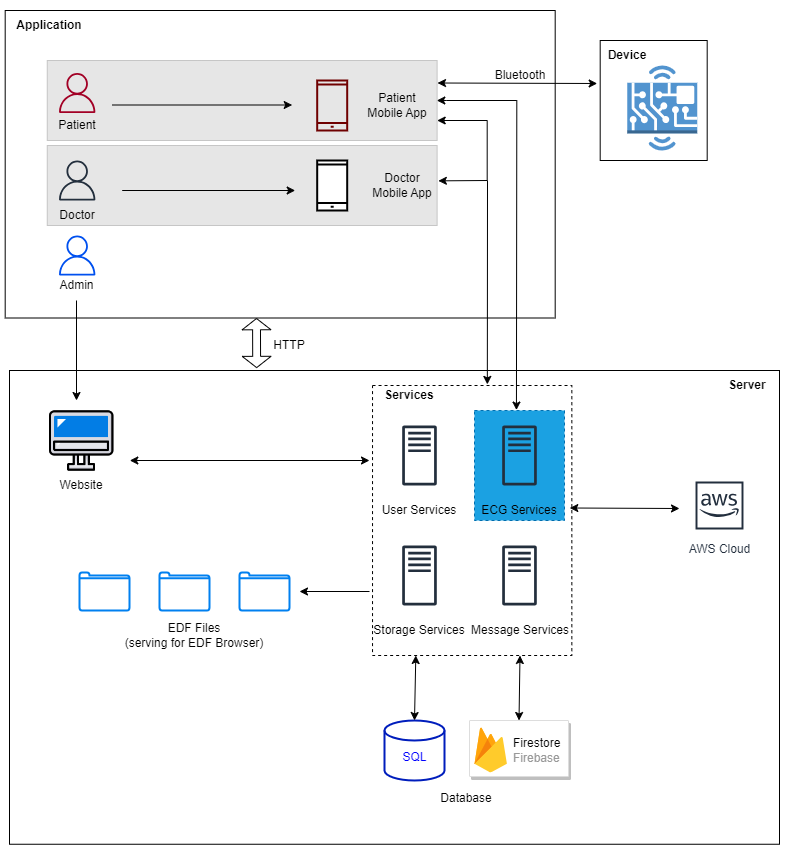
\includegraphics[width=16cm,height=18cm]{Images/system/fmECG_architecture-System Architecture.drawio.png}
  \caption[Kiến trúc tổng quan hệ thống]{\bfseries \fontsize{12pt}{0pt}\selectfont Kiến trúc tổng quan hệ thống}
  \label{fmECG_architecture-System} %đặt tên cho ảnh
\end{figure}

Hình \ref{fmECG_architecture-System} thể hiện ba phần: 
\begin{itemize}
  \item Device: Thiết bị phần cứng đo điện tim, để kết nối với App bệnh nhân thông qua Bluetooth 
  \item Application: Bao gồm ứng dụng của bệnh nhân, ứng dụng của bác sĩ và Website của Admin
  \item Server: Bao gồm các Services để xử lý các yêu cầu gửi từ Application, cơ sở dữ liệu và Cloud lưu trữ
\end{itemize}

Trong hệ thống thì Devices là phần mà chúng em sẽ không trực tiếp thực hiện trong đồ án này, Application và Server sẽ là
phần mà đồ án chúng em thực hiện. Ở trong sơ đồ kiến trúc hệ thống riêng có bệnh nhân sẽ có tương tác trực tiếp với Devices,
còn lại khối Application sẽ tương tác với Server thông qua API với giao thức HTTP. Khi nhận được yêu cầu từ Application,
Server sẽ thực hiện xử lý dữ liệu, mọi yêu cầu đến đều được xử lý bởi Services, tuỳ vào yêu cầu đến Services tương ứng sẽ đảm nhiệm 
việc lấy/lưu dữ liệu trong cơ sở dữ liệu sau đó trả ra kết quả cho người dùng.

Ngoài ra, hệ thống sẽ phải có kết nối bluetooth low energy giữa thiết bị đo và ứng dụng di động để có thể truyền/nhận dữ liệu.
Trên đây là tổng quan về kiến trúc hệ thống, phần tiếp dưới đây chúng em xin phép trình bày kỹ hơn về từng khối nhỏ hơn
dựa vào những đối tượng đã được xác định trong hệ thống.

\subsection{Sơ đồ khối phần mềm}

\subsubsection{Ứng dụng di động cho bệnh nhân}
\mbox{}

\begin{figure}[H]
  \centering
  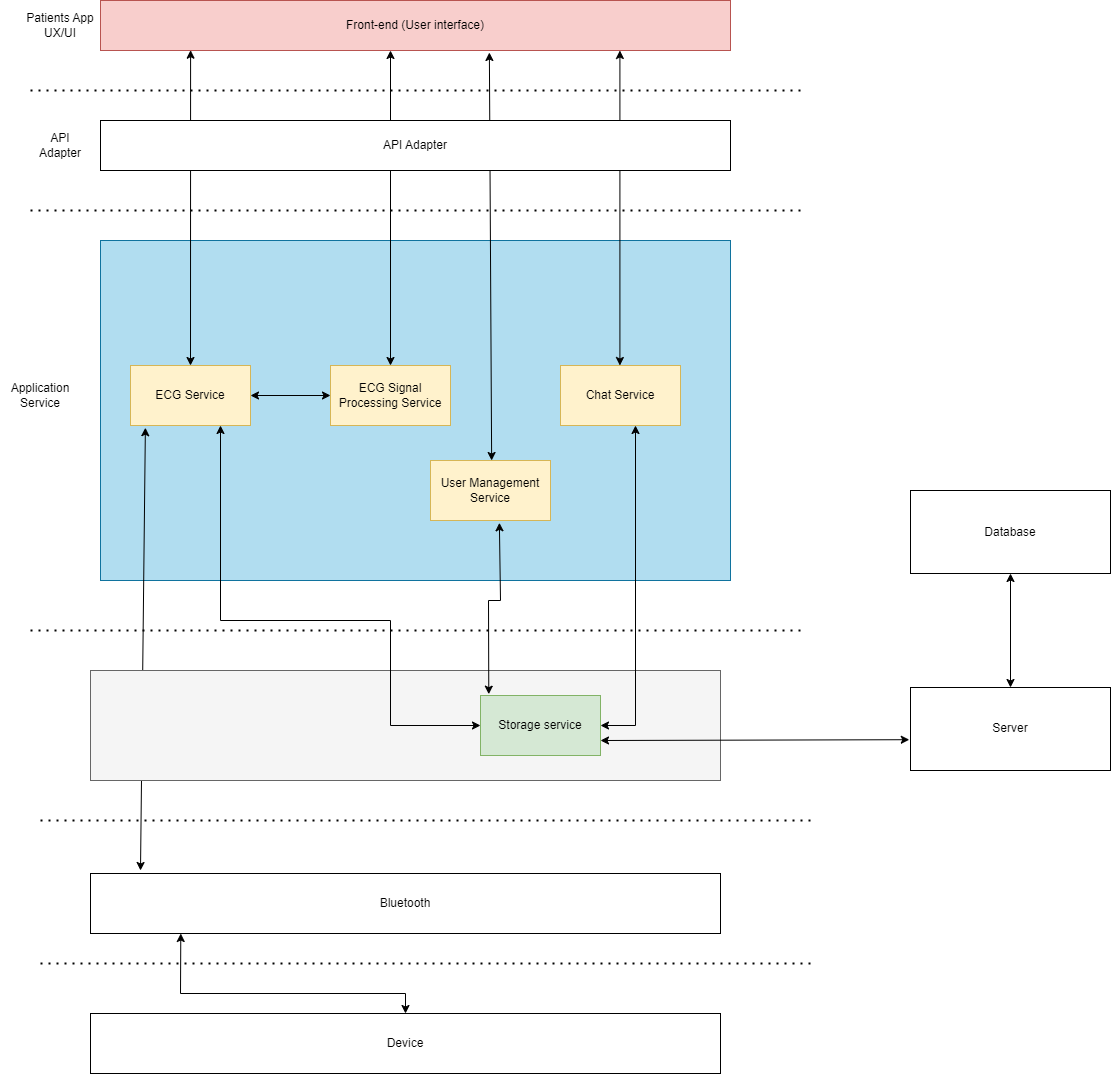
\includegraphics[width=16cm,height=18cm]{Images/system/fmECG_architecture-Patient.drawio.png}
  \caption[Sơ đồ khối cho App bệnh nhân]{\bfseries \fontsize{12pt}{0pt}\selectfont Sơ đồ khối cho App bệnh nhân}
  \label{fmECG_architecture-Patient} %đặt tên cho ảnh
\end{figure}

Trong hình trên, lớp trên cùng User interface là lớp để người dùng tương tác và thực hiện lời gọi thông qua API Adapter, 
các yêu cầu của người dùng sẽ được xử lý thông qua Services và phản hồi lại với người dùng qua giao diện. Dưới đây là phần
giải thích Services trong hình:

\begin{itemize}
  \item ECG Service: Khối có nhiệm vụ xử lý yêu cầu cho các trạng thái đo: thực hiện đo, kết thúc đo, lưu kết quả đo
  \item ECG Signal Processing Service: Khối có nhiệm vụ xử lý tín hiệu đo để phân tích sâu, hiển thị lên màn hình
  \item User Management Service: Khối có nhiệm vụ xử lý các vấn đề liên quan đến người dùng như đăng nhập, đăng ký
  \item Chat Service: Khối có nhiệm vụ quản lý việc chat, trao đổi thông tin
  \item Storage Service: Khối có nhiệm vụ lưu thông tin vào bộ nhớ
\end{itemize}

Riêng với App cho bệnh nhân thì sẽ có Khối Bluetooth và Khối Device để phục vụ cho việc đo điện tim.
\subsubsection{Ứng dụng di động cho bác sĩ}

\begin{figure}[H]
  \centering
  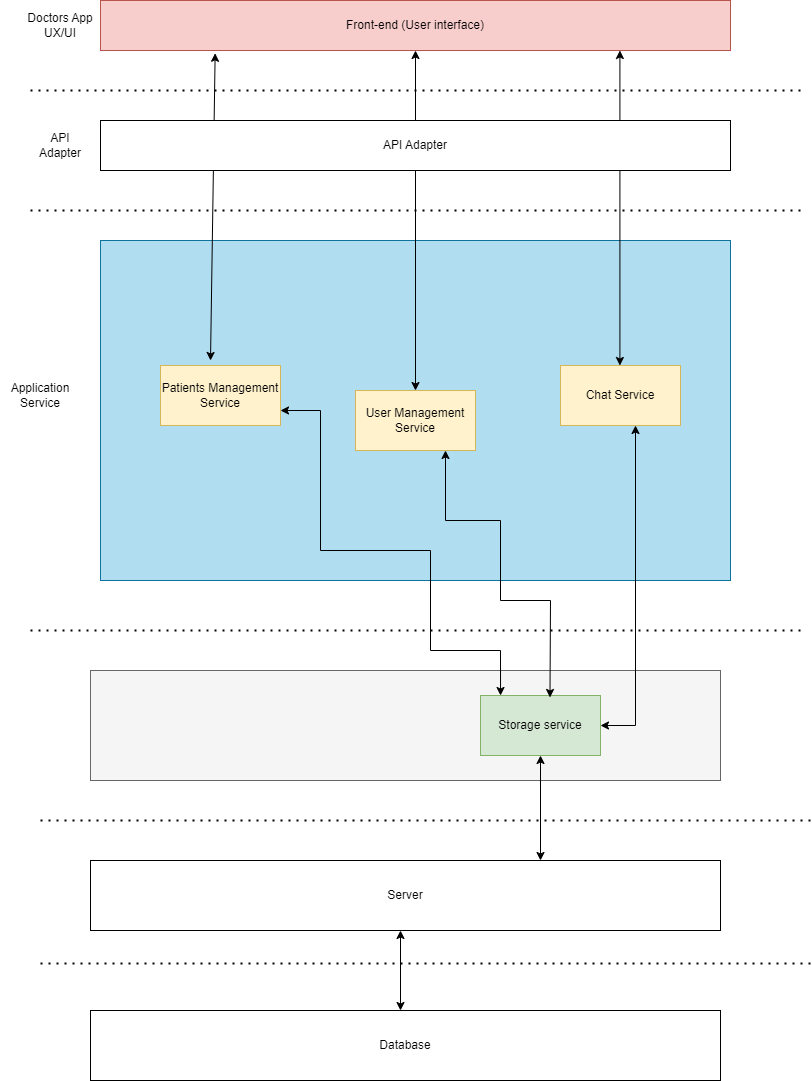
\includegraphics[width=16cm,height=18cm]{Images/system/fmECG_architecture-Doctors.drawio.png}
  \caption[Sơ đồ khói cho App bác sĩ]{\bfseries \fontsize{12pt}{0pt}\selectfont Sơ đồ khối cho App bác sĩ}
  \label{fmECG_architecture-Doctors} %đặt tên cho ảnh
\end{figure}

Về cơ bản, ứng dụng di động cho bác sĩ có những khối tương tự với bệnh nhân, trừ việc bác sĩ sẽ không có hai khối Device
và Bluetooth để phục vụ việc đo như bệnh nhân.


\subsubsection{Website cho quản trị viên}

\begin{figure}[H]
  \centering
  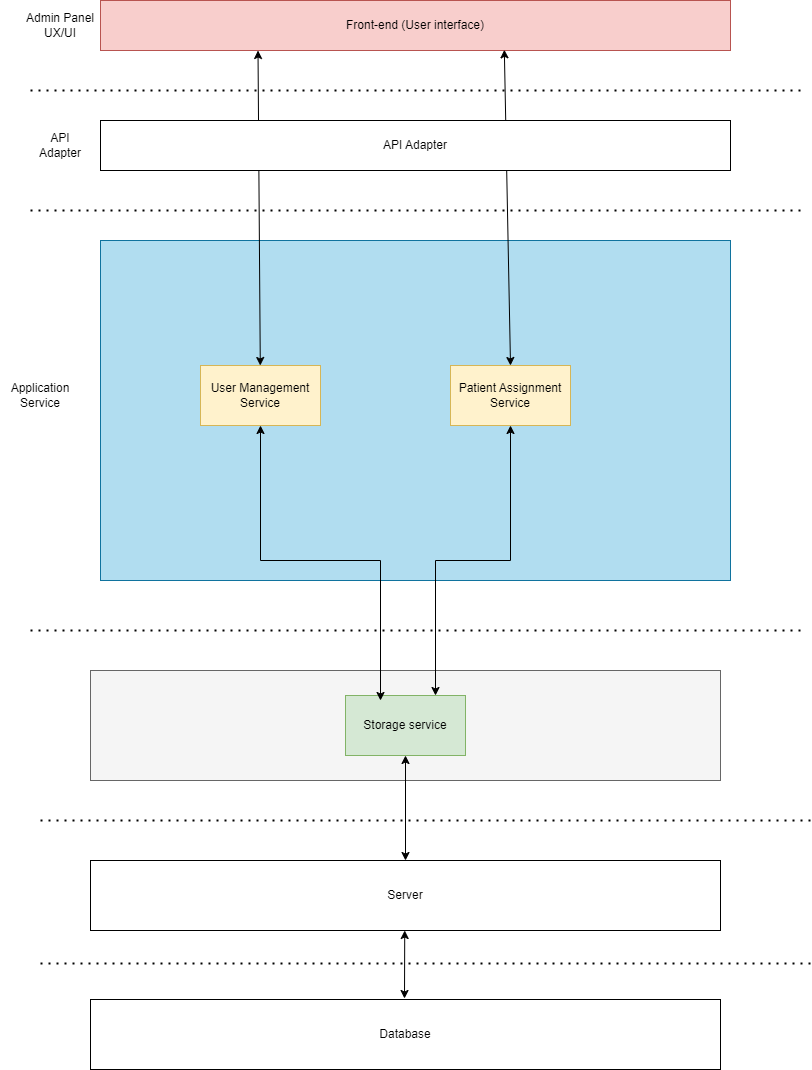
\includegraphics[width=16cm,height=18cm]{Images/system/fmECG_architecture-Admin.drawio.png}
  \caption[Sơ đồ khối cho Website quản trị viên]{\bfseries \fontsize{12pt}{0pt}\selectfont Sơ đồ khối cho Website quản trị viên}
  \label{fmECG_architecture-Admin} %đặt tên cho ảnh
\end{figure}

Quản trị viên sẽ quản lý 2 Services chính đó là quản lý người dùng (User Management Service) và quản lý phân công
bác sĩ - bệnh nhân (Patient Assignment Service), logic và thứ tự các khối tương đồng với ứng dụng dành cho bác sĩ.

Tiếp theo để phân tích cụ thể hơn từng luồng trong hệ thống qua use case, chúng em xin phép được trình bày các sơ đồ tuần
tự. 
\newpage


\subsection{Thiết kế cơ sở dữ liệu}
\label{design_database}


\subsubsection{Chuyển mô hình thực thể liên kết sang mô hình quan hệ}

\begin{itemize}
  \item Người dùng (\textbf{ID người dùng}, Mật khẩu, Email, Tên, Ngày sinh, Số điện thoại, Quyền)
  \item Bản ghi ECG (\textbf{ID bản ghi ECG}, ID người dùng, ID thiết bị, Đường dẫn lưu trữ dữ liệu, Thời gian bắt đầu đo, Thời gian kết thúc đo, Loại cảm biến)
  \item Danh mục tin tức (\textbf{ID danh mục tin tức}, Tên danh mục tin tức, Mô tả danh mục tin tức)
  \item Tin tức (\textbf{ID tin tức}, Tiêu đề, Nội dung, ID danh mục tin tức, Tác giả, Đường dẫn, Đường dẫn hình ảnh)
  \item Phân công bệnh nhân - bác sĩ (\textbf{ID phân công}, ID bệnh nhân, ID bác sĩ, Ngày bắt đầu)
  \item Mã thông báo đặt lại mật khẩu (\textbf{ID mã thông báo}, ID người dùng, Mã thông báo, Thời gian hết hạn)
  \item Phiên đăng nhập (\textbf{ID phiên đăng nhập}, ID người dùng, Mã phiên đăng nhập, Thời gian hết hạn)
  \item Thiết bị (\textbf{ID thiết bị}, Tên thiết bị)
\end{itemize}



\subsubsection{Mối quan hệ dữ liệu}

\begin{itemize}
  \item Bảng \texttt{ecg\_record} có mối quan hệ 1-n với bảng \texttt{user} thông qua khóa ngoại \texttt{user\_id}.
  \item Bảng \texttt{news} có mối quan hệ n-1 với bảng \texttt{news\_category} thông qua khóa ngoại \texttt{category\_id}.
  \item Bảng \texttt{patient\_doctor\_assignment} có mối quan hệ n-1 với bảng \texttt{user} thông qua khóa ngoại \texttt{patient\_id} và \texttt{doctor\_id}.
  \item Bảng \texttt{reset\_token} có mối quan hệ n-1 với bảng \texttt{user} thông qua khóa ngoại \texttt{user\_id}.
\end{itemize}

\subsubsection{Chuẩn hoá 3NF}
Các bảng đã được thiết kế theo nguyên tắc chuẩn hoá 3NF, vì không có thuộc tính lặp lại và các thuộc tính không phụ thuộc vào một tập hợp con của khóa chính.

\paragraph{Chuẩn hoá bảng Người dùng}
\mbox{}

\begin{table}[H]
  \caption{\bfseries \fontsize{12pt}{0pt}\selectfont Bảng chuẩn hoá bảng Người dùng}
  \centering
  \begin{tabularx}{0.9\textwidth}{|X|X|}
    \hline
    \textbf{Danh sách thuộc tính} & ID người dùng, Mật khẩu, Email, Tên, Ngày sinh, Số điện thoại,
    Quyền \\ % Thêm \textbf{} cho abc
    \hline
    \textbf{Quy tắc nghiệp vụ} & \textbf{Phụ thuộc hàm} \\
    \hline
    Mỗi người dùng có một ID riêng, có duy nhất mật khẩu, email, tên, ngày sinh, số điện thoại,
    quyền & \parbox[t]{\linewidth}{$\text{ID người dùng} \rightarrow$ mật khẩu, email, tên, ngày sinh, số điện thoại, quyền} \\
    \hline
    \multicolumn{2}{|X|}{$\Rightarrow \text{Khoá chính của bảng: ID người dùng}$} \\
    \multicolumn{2}{|X|}{$\Rightarrow \text{Bảng Người dùng đã ở 3NF}$} \\
    \hline
  \end{tabularx}
\end{table}


\paragraph{Chuẩn hoá bảng Bản ghi ECG}
\mbox{}

\begin{table}[H]
  \caption{\bfseries \fontsize{12pt}{0pt}\selectfont Bảng chuẩn hoá bảng Bản ghi ECG}
  \centering
  \begin{tabularx}{0.9\textwidth}{|X|X|}
    \hline
    \textbf{Danh sách thuộc tính} & ID bản ghi ECG, ID người dùng, ID thiết bị, Đường dẫn lưu trữ dữ
    liệu, Thời gian bắt đầu đo, Thời gian kết thúc đo, Loại cảm biến \\
    \hline
    \textbf{Quy tắc nghiệp vụ} & \textbf{Phụ thuộc hàm} \\
    \hline
    Mỗi bản ghi ECG có một ID riêng, có duy nhất ID người dùng, ID thiết bị, đường dẫn lưu trữ dữ
    liệu, thời gian bắt đầu đo, thời gian kết thúc đo, loại cảm biến & \parbox[t]{\linewidth}{$ \text{ID bản ghi ECG} \rightarrow$ ID người dùng, ID thiết bị, đường dẫn lưu trữ dữ
    liệu, thời gian bắt đầu đo, thời gian kết thúc đo, loại cảm biến} \\
    \hline
    \multicolumn{2}{|X|}{$\Rightarrow \text{Khoá chính của bảng: ID bản ghi ECG}$} \\
    \multicolumn{2}{|X|}{$\Rightarrow \text{Bảng Bản ghi ECG đã ở 3NF}$} \\
    \hline
  \end{tabularx}
\end{table}


\paragraph{Chuẩn hoá bảng Danh mục tin tức}
\mbox{}


\begin{table}[H]
  \caption{\bfseries \fontsize{12pt}{0pt}\selectfont Bảng chuẩn hoá bảng Danh mục tin tức}
  \centering
  \begin{tabularx}{0.9\textwidth}{|X|X|}
    \hline
    \textbf{Danh sách thuộc tính} & ID danh mục tin tức, Tên danh mục tin tức, Mô tả danh mục tin
    tức \\ % Thêm \textbf{} cho abc
    \hline
    \textbf{Quy tắc nghiệp vụ} & \textbf{Phụ thuộc hàm} \\
    \hline
    Mỗi danh mục tin tức có một ID riêng, có duy nhất tên danh mục tin tức, mô tả danh mục tin
    tức & \parbox[t]{\linewidth}{$\text{ID danh mục tin tức} \rightarrow$ danh mục tin tức, mô tả danh mục tin
    tức} \\
    \hline
    \multicolumn{2}{|X|}{$\Rightarrow \text{Khoá chính của bảng: ID danh mục tin tức}$} \\
    \multicolumn{2}{|X|}{$\Rightarrow \text{Bảng Danh mục tin tức đã ở 3NF}$} \\
    \hline
  \end{tabularx}
\end{table}


\paragraph{Chuẩn hoá bảng Tin tức}
\mbox{}

\begin{table}[H]
  \caption{\bfseries \fontsize{12pt}{0pt}\selectfont Bảng chuẩn hoá bảng Tin tức}
  \centering
  \begin{tabularx}{0.9\textwidth}{|X|X|}
    \hline
    \textbf{Danh sách thuộc tính} & ID tin tức, Tiêu đề, Nội dung, ID danh mục tin tức, Tác giả, Đường dẫn,
    Đường dẫn hình ảnh \\ % Thêm \textbf{} cho abc
    \hline
    \textbf{Quy tắc nghiệp vụ} & \textbf{Phụ thuộc hàm} \\
    \hline
    Mỗi tin tức có một ID riêng, có duy nhất tiêu đề, nội dung, ID danh mục tin tức, tác giả, đường dẫn,
    đường dẫn hình ảnh & \parbox[t]{\linewidth}{$\text{ID tin tức} \rightarrow$ tiêu đề, nội dung, ID danh mục tin tức, tác giả, đường dẫn,
    đường dẫn hình ảnh} \\
    \hline
    \multicolumn{2}{|X|}{$\Rightarrow \text{Khoá chính của bảng: ID tin tức}$} \\
    \multicolumn{2}{|X|}{$\Rightarrow \text{Bảng Tin tức đã ở 3NF}$} \\
    \hline
  \end{tabularx}
\end{table}



\paragraph{Chuẩn hoá bảng Phân công bệnh nhân - bác sĩ}
\mbox{}

\begin{table}[H]
  \caption{\bfseries \fontsize{12pt}{0pt}\selectfont Bảng chuẩn hoá bảng Phân công bệnh nhân - bác sĩ}
  \centering
  \begin{tabularx}{0.9\textwidth}{|X|X|}
    \hline
    \textbf{Danh sách thuộc tính} & ID phân công, ID bệnh nhân, ID bác sĩ, Ngày bắt
    đầu \\ % Thêm \textbf{} cho abc
    \hline
    \textbf{Quy tắc nghiệp vụ} & \textbf{Phụ thuộc hàm} \\
    \hline
    Mỗi lần phân công bệnh nhân - bác sĩ có một ID riêng, có duy nhất ID bệnh nhân, ID bác sĩ, ngày bắt
    đầu & \parbox[t]{\linewidth}{$\text{ID phân công} \rightarrow$ ID bệnh nhân, ID bác sĩ, ngày bắt
    đầu} \\
    \hline
    \multicolumn{2}{|X|}{$\Rightarrow \text{Khoá chính của bảng: ID phân công}$} \\
    \multicolumn{2}{|X|}{$\Rightarrow \text{Bảng Phân công bệnh nhân - bác sĩ đã ở 3NF}$} \\
    \hline
  \end{tabularx}
\end{table}




\paragraph{Chuẩn hoá bảng Mã thông báo đặt lại mật khẩu}
\mbox{}

\begin{table}[H]
  \caption{\bfseries \fontsize{12pt}{0pt}\selectfont Bảng chuẩn hoá bảng Mã thông báo đặt lại mật khẩu}
  \centering
  \begin{tabularx}{0.9\textwidth}{|X|X|}
    \hline
    \textbf{Danh sách thuộc tính} & ID mã thông báo, ID người dùng, Mã thông báo,
    Thời gian hết hạn \\ % Thêm \textbf{} cho abc
    \hline
    \textbf{Quy tắc nghiệp vụ} & \textbf{Phụ thuộc hàm} \\
    \hline
    Mỗi mã thông báo đặt lại mật khẩu có một ID riêng, có duy nhất ID người dùng, mã thông báo,
    thời gian hết hạn & \parbox[t]{\linewidth}{$\text{ID mã thông báo} \rightarrow$ ID người dùng, mã thông báo,
    thời gian hết hạn} \\
    \hline
    \multicolumn{2}{|X|}{$\Rightarrow \text{Khoá chính của bảng: ID mã thông báo}$} \\
    \multicolumn{2}{|X|}{$\Rightarrow \text{Bảng Mã thông báo đặt lại mật khẩu đã ở 3NF}$} \\
    \hline
  \end{tabularx}
\end{table}


\paragraph{Chuẩn hoá bảng Phiên đăng nhập}
\mbox{}

\begin{table}[H]
  \caption{\bfseries \fontsize{12pt}{0pt}\selectfont Bảng chuẩn hoá bảng Phiên đăng nhập}
  \centering
  \begin{tabularx}{0.9\textwidth}{|X|X|}
    \hline
    \textbf{Danh sách thuộc tính} & ID phiên đăng nhập, ID người dùng, Mã phiên đăng nhập, Thời
    gian hết hạn \\ % Thêm \textbf{} cho abc
    \hline
    \textbf{Quy tắc nghiệp vụ} & \textbf{Phụ thuộc hàm} \\
    \hline
    Mỗi phiên đăng nhập có một ID riêng, có duy nhất ID người dùng, mã phiên đăng nhập, thời
    gian hết hạn & \parbox[t]{\linewidth}{$\text{ID phiên đăng nhập} \rightarrow$ ID người dùng, mã phiên đăng nhập, thời
    gian hết hạn} \\
    \hline
    \multicolumn{2}{|X|}{$\Rightarrow \text{Khoá chính của bảng: ID phiên đăng nhập}$} \\
    \multicolumn{2}{|X|}{$\Rightarrow \text{Bảng Phiên đăng nhập đã ở 3NF}$} \\
    \hline
  \end{tabularx}
\end{table}



\paragraph{Chuẩn hoá bảng Thiết bị}
\mbox{}

\begin{table}[H]
  \caption{\bfseries \fontsize{12pt}{0pt}\selectfont Bảng chuẩn hoá bảng Thiết bị}
  \centering
  \begin{tabularx}{0.9\textwidth}{|X|X|}
    \hline
    \textbf{Danh sách thuộc tính} & ID thiết bị, Tên thiết bị \\ % Thêm \textbf{} cho abc
    \hline
    \textbf{Quy tắc nghiệp vụ} & \textbf{Phụ thuộc hàm} \\
    \hline
    Mỗi thiết bị có một ID riêng, có duy nhất tên thiết bị & \parbox[t]{\linewidth}{$\text{ID thiết bị} \rightarrow$ tên thiết bị} \\
    \hline
    \multicolumn{2}{|X|}{$\Rightarrow \text{Khoá chính của bảng: ID thiết bị}$} \\
    \multicolumn{2}{|X|}{$\Rightarrow \text{Bảng Thiết bị đã ở 3NF}$} \\
    \hline
  \end{tabularx}
\end{table}




\subsubsection{Từ điển dữ liệu}



\begin{table}[H]
  \caption{\bfseries \fontsize{12pt}{0pt}\selectfont Bảng user}
  \centering
  \begin{tabularx}{0.9\textwidth}{|c|c|X|}
    \hline
    \textbf{Thuộc tính} & \textbf{Kiểu dữ liệu} & \textbf{Mô tả} \\
    \hline
    user\_id & INTEGER & Khóa chính của bảng, đại diện cho ID người dùng. \\
    \hline
    password & STRING & Mật khẩu của người dùng. \\
    \hline
    email & STRING & Địa chỉ email của người dùng. \\
    \hline
    name & STRING & Tên của người dùng. \\
    \hline
    doB & DATE & Ngày sinh của người dùng. \\
    \hline
    phone\_number & STRING & Số điện thoại của người dùng. \\
    \hline
    role & INTEGER & Quyền của người dùng (0-patient, 1-doctor, 2-admin). \\
    \hline
    created\_at & DATE & Thời điểm thêm mới dữ liệu vào database. \\
    \hline
    updated\_at & DATE & Thời điểm cập nhật dữ liệu vào database. \\
    \hline
    
  \end{tabularx}
\end{table}

\begin{table}[H]
  \caption{\bfseries \fontsize{12pt}{0pt}\selectfont Bảng ecg\_record}
  \centering
  \begin{tabularx}{0.9\textwidth}{|c|c|X|}
    \hline
    \textbf{Thuộc tính} & \textbf{Kiểu dữ liệu} & \textbf{Mô tả} \\
    \hline
    record\_id & INTEGER & Khóa chính của bảng, đại diện cho ID bản ghi ECG. \\
    \hline
    user\_id & INTEGER & Khóa ngoại tham chiếu đến \texttt{user\_id} trong bảng \texttt{user}. \\
    \hline
    device\_id & STRING & ID thiết bị. \\
    \hline
    data\_directory & STRING & Đường dẫn lưu trữ dữ liệu. \\
    \hline
    start\_time & DATE & Thời gian bắt đầu ghi lại ECG. \\
    \hline
    stop\_time & DATE & Thời gian kết thúc ghi lại ECG. \\
    \hline
    sensor\_type & STRING & Loại cảm biến. \\
    \hline
    created\_at & DATE & Thời điểm thêm mới dữ liệu vào database. \\
    \hline
    updated\_at & DATE & Thời điểm cập nhật dữ liệu vào database. \\
    \hline
  \end{tabularx}
\end{table}

\begin{table}[H]
  \caption{\bfseries \fontsize{12pt}{0pt}\selectfont Bảng news\_category}
  \centering
  \begin{tabularx}{0.9\textwidth}{|c|c|X|}
    \hline
    \textbf{Thuộc tính} & \textbf{Kiểu dữ liệu} & \textbf{Mô tả} \\
    \hline
    category\_id & INTEGER & Khóa chính của bảng, đại diện cho ID danh mục tin tức. \\
    \hline
    category\_name & STRING & Tên danh mục tin tức. \\
    \hline
    category\_description & STRING & Mô tả danh mục tin tức. \\
    \hline
    created\_at & DATE & Thời điểm thêm mới dữ liệu vào database. \\
    \hline
    updated\_at & DATE & Thời điểm cập nhật dữ liệu vào database. \\
    \hline
  \end{tabularx}
\end{table}

\begin{table}[H]
  \caption{\bfseries \fontsize{12pt}{0pt}\selectfont Bảng news}
  \centering
  \begin{tabularx}{0.9\textwidth}{|c|c|X|}
    \hline
    \textbf{Thuộc tính} & \textbf{Kiểu dữ liệu} & \textbf{Mô tả} \\
    \hline
    news\_id & INTEGER & Khóa chính của bảng, đại diện cho ID tin tức. \\
    \hline
    title & STRING & Tiêu đề tin tức. \\
    \hline
    content & TEXT & Nội dung tin tức. \\
    \hline
    category\_id & INTEGER & Khóa ngoại tham chiếu đến \texttt{category\_id} trong bảng \texttt{news\_category}. \\
    \hline
    author & STRING & Tác giả tin tức. \\
    \hline
    url & STRING & Đường dẫn tin tức. \\
    \hline
    image & STRING & Đường dẫn hình ảnh tin tức (có thể là null). \\
    \hline
    created\_at & DATE & Thời điểm thêm mới dữ liệu vào database. \\
    \hline
    updated\_at & DATE & Thời điểm cập nhật dữ liệu vào database. \\
    \hline
  \end{tabularx}
\end{table}

\begin{table}[H]
  \caption{\bfseries \fontsize{12pt}{0pt}\selectfont Bảng patient\_doctor\_assignment}
  \centering
  \begin{tabularx}{0.9\textwidth}{|c|c|X|}
    \hline
    \textbf{Thuộc tính} & \textbf{Kiểu dữ liệu} & \textbf{Mô tả} \\
    \hline
    assign\_id & INTEGER & Khóa chính của bảng, đại diện cho ID phân công bệnh nhân - bác sĩ. \\
    \hline
    patient\_id & INTEGER & Khóa ngoại tham chiếu đến \texttt{user\_id} trong bảng \texttt{user} (với quyền là bệnh nhân). \\
    \hline
    doctor\_id & INTEGER & Khóa ngoại tham chiếu đến \texttt{user\_id} trong bảng \texttt{user} (với quyền là bác sĩ). \\
    \hline
    start\_date & DATE & Ngày bắt đầu phân công. \\
    \hline
    created\_at & DATE & Thời điểm thêm mới dữ liệu vào database. \\
    \hline
    updated\_at & DATE & Thời điểm cập nhật dữ liệu vào database. \\
    \hline
  \end{tabularx}
\end{table}

\begin{table}[H]
  \caption{\bfseries \fontsize{12pt}{0pt}\selectfont Bảng reset\_token}
  \centering
  \begin{tabularx}{0.9\textwidth}{|c|c|X|}
    \hline
    \textbf{Thuộc tính} & \textbf{Kiểu dữ liệu} & \textbf{Mô tả} \\
    \hline
    id & INTEGER & Khóa chính của bảng, đại diện cho ID mã thông báo đặt lại. \\
    \hline
    user\_id & INTEGER & Khóa ngoại tham chiếu đến \texttt{user\_id} trong bảng \texttt{user}. \\
    \hline
    token & STRING & Mã thông báo đặt lại. \\
    \hline
    expiration & DATE & Thời gian hết hạn của mã thông báo đặt lại. \\
    \hline
    created\_at & DATE & Thời điểm thêm mới dữ liệu vào database. \\
    \hline
    updated\_at & DATE & Thời điểm cập nhật dữ liệu vào database. \\
    \hline
  \end{tabularx}
\end{table}


\begin{table}[H]
  \caption{\bfseries \fontsize{12pt}{0pt}\selectfont Bảng session}
  \centering
  \begin{tabularx}{0.9\textwidth}{|c|c|X|}
    \hline
    \textbf{Thuộc tính} & \textbf{Kiểu dữ liệu} & \textbf{Mô tả} \\
    \hline
    session\_id & INTEGER & Khóa chính của bảng, đại diện cho ID phiên đăng nhập. \\
    \hline
    user\_id & INTEGER & Khóa ngoại tham chiếu đến \texttt{user\_id} trong bảng \texttt{user}. \\
    \hline
    token & STRING & Mã phiên đăng nhập. \\
    \hline
    expiration & DATE & Thời gian hết hạn của phiên đăng nhập. \\
    \hline
    created\_at & DATE & Thời điểm thêm mới dữ liệu vào database. \\
    \hline
    updated\_at & DATE & Thời điểm cập nhật dữ liệu vào database. \\
    \hline
  \end{tabularx}
\end{table}

\begin{table}[H]
  \caption{\bfseries \fontsize{12pt}{0pt}\selectfont Bảng device}
  \centering
  \begin{tabularx}{0.9\textwidth}{|c|c|X|}
    \hline
    \textbf{Thuộc tính} & \textbf{Kiểu dữ liệu} & \textbf{Mô tả} \\
    \hline
    device\_id & INTEGER & Khóa chính của bảng, đại diện cho ID thiết bị. \\
    \hline
    device\_name & STRING & Tên thiết bị. \\
    \hline
    created\_at & DATE & Thời điểm thêm mới dữ liệu vào database. \\
    \hline
    updated\_at & DATE & Thời điểm cập nhật dữ liệu vào database. \\
    \hline
  \end{tabularx}
\end{table}

\subsubsection{Sơ đồ ERD}

\begin{figure}[H]
  \centering
  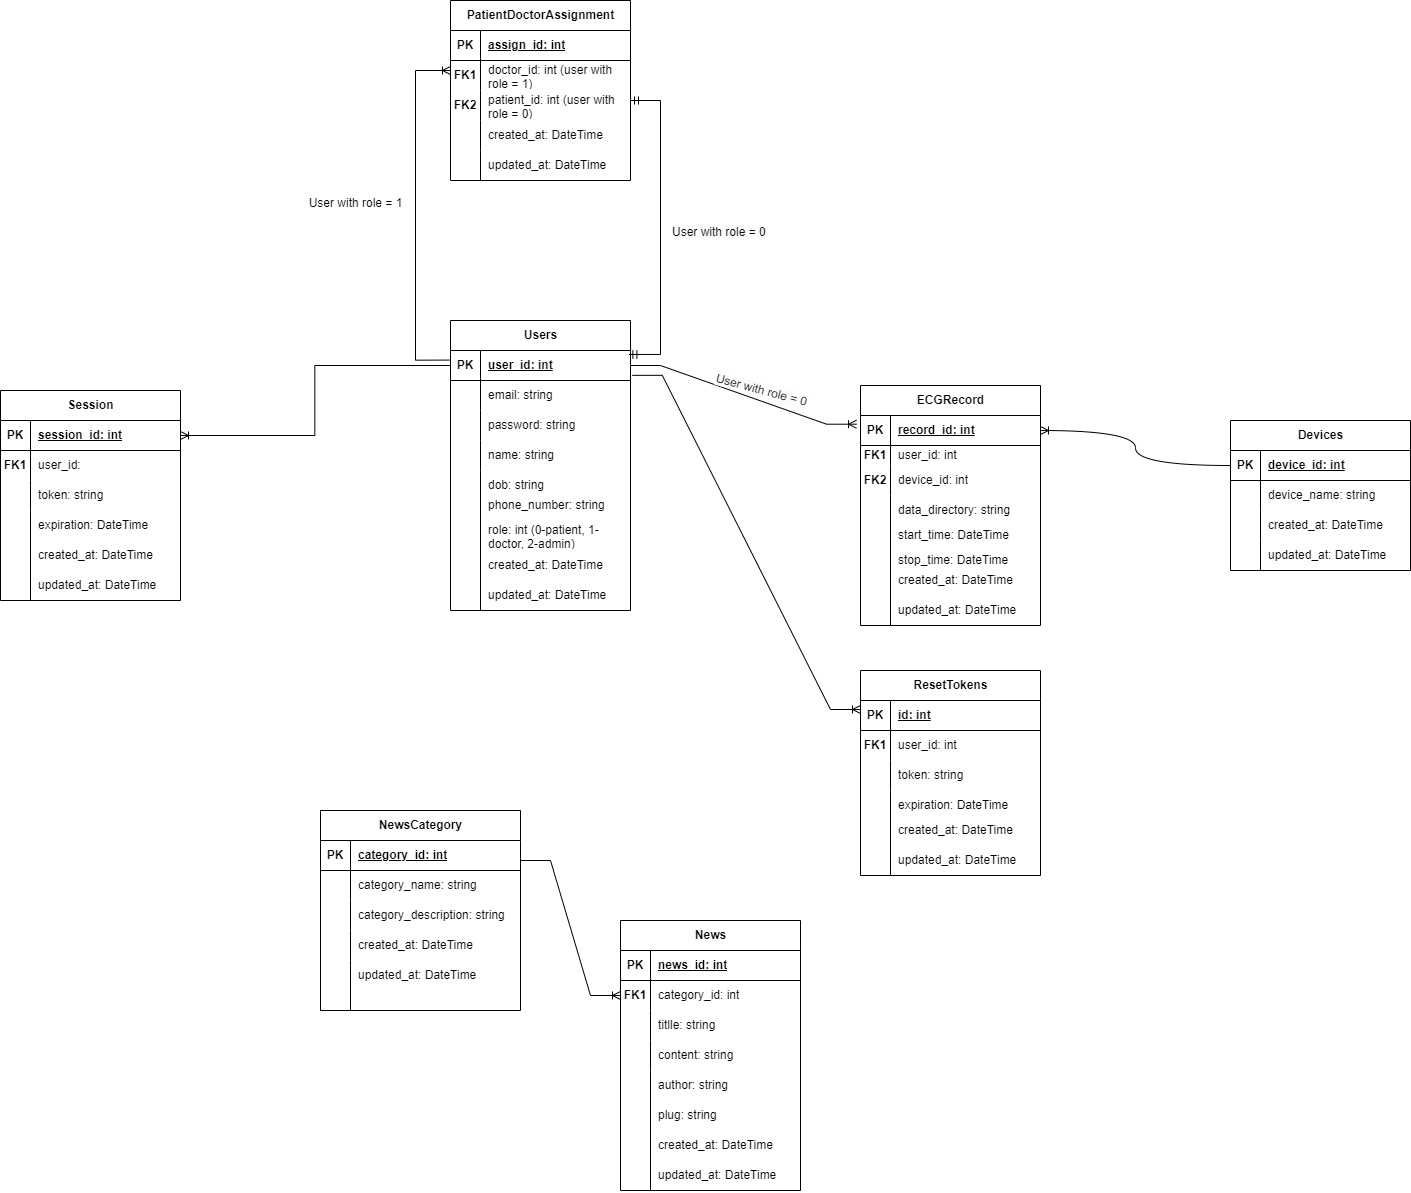
\includegraphics[width=15cm,height=15cm]{Images/server/database/fmECG_architecture-Database.drawio.png}
  \caption[Sơ đồ ERD]{\bfseries \fontsize{12pt}{0pt}\selectfont Sơ đồ ERD}
  \label{fmECG_architecture-Database} %đặt tên cho ảnh
\end{figure}


\subsection{Thiết kế chi tiết hệ thống}

\subsubsection{Sơ đồ lớp cho ứng dụng di động, website và server}

\paragraph{Ứng dụng di động}
\mbox{}

Ứng dụng di động được tổ chức theo mô hình MVC, với ba khối chính là Models, Views và Controllers:
  
\begin{itemize}
  \item Khối "Models": Chứa các lớp đại diện cho các đối tượng của cơ sở dữ liệu, định nghĩa các thuộc tính và phương thức để làm việc với dữ liệu.
 
  \item Khối "Controllers": Chứa các controllers xử lý logic và điều khiển các yêu cầu từ người dùng.

  \item Khối "Views": Chứa các lớp route, xác định các endpoint và xử lý các yêu cầu HTTP từ người dùng bằng cách gọi tới các controllers tương ứng.
\end{itemize}

Chi tiết từng lớp và phần giải thích cho mỗi khối được chúng em thể hiện bằng hình và lời trong các mục bên dưới. 

\begin{enumerate}[a)]
  \item Danh sách các class diagram cho ứng dụng di động
    
  \begin{figure}[H]
    \centering
    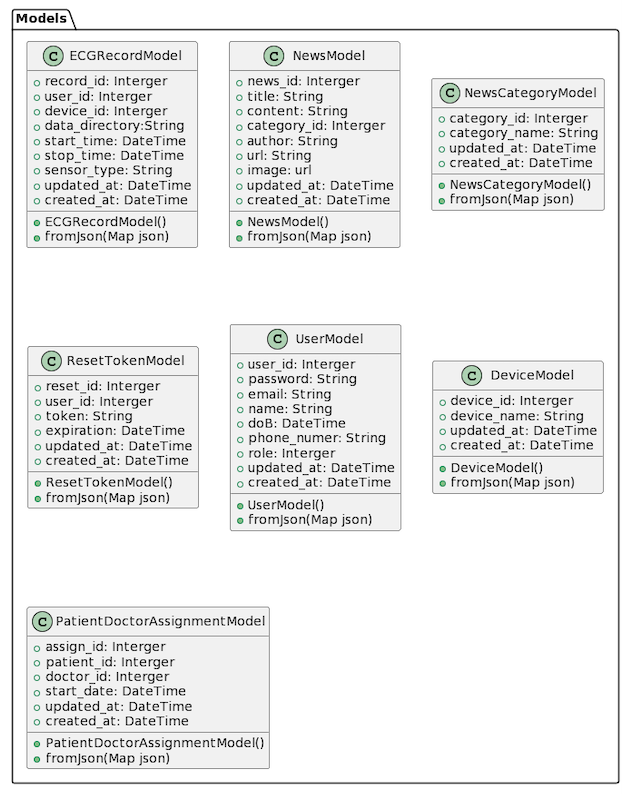
\includegraphics[width=16cm,height=18cm]{Images/mobile_app/class_diagram/mobile_class_model.png}
    \caption[Sơ đồ lớp của khối Models trong ứng dụng di động]{\bfseries \fontsize{12pt}{0pt}\selectfont Sơ đồ lớp của khối Models trong ứng dụng di động}
    \label{mobile_class_model} %đặt tên cho ảnh
  \end{figure}

  Dựa trên mục \ref{design_database} về phần thiết kế cơ sở dữ liệu, Hình \ref{mobile_class_model} thể hiện các lớp trong Models:
  \begin{itemize}
    \item ECGRecordModel: Lớp thể hiện cấu trúc của một bản ghi dữ liệu điện tim
    \item NewsModel: Lớp thể hiện cấu trúc một tin tức
    \item NewsCategoryModel: Lớp thể hiện cấu trúc một danh mục tin tức
    \item UserModel: Lớp thể hiện cho cấu trúc người dùng trong hệ thống
    \item DeviceModel: Lớp thể hiện cho thông tin thiết bị điện tim 
    \item PatientDoctorAssignmentModel: Lớp thể hiện cho thông tin phân công bác sĩ và bệnh nhân.
  \end{itemize}

  Mỗi lớp đều có một hàm fromJSON để chuyển từ dữ liệu JSON lấy từ API vào trong Model tương ứng. Điều này giúp
  việc code và xử lý trở nên dễ dàng hơn. Sau khi định nghĩa được các Model.
  
  Phần tiếp theo là xác định các Views hay giao diện cần có trong ứng dụng di động và Controllers xử lý logic với những
  yêu cầu từ người dùng.

  \begin{figure}[H]
    \centering
    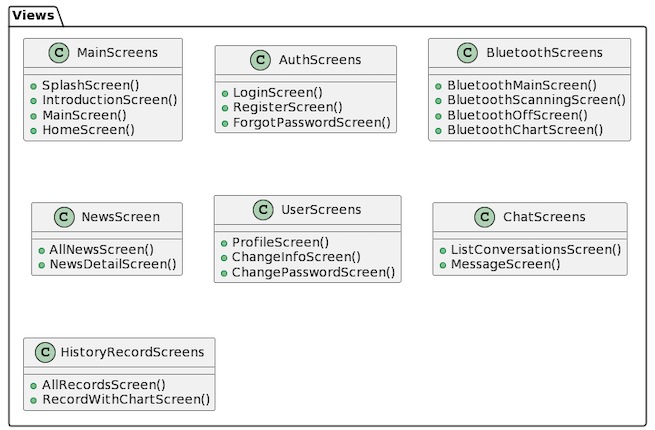
\includegraphics[width=14cm,height=7cm]{Images/mobile_app/class_diagram/mobile_class_view.png}
    \caption[Sơ đồ lớp của khối Views trong ứng dụng di động]{\bfseries \fontsize{12pt}{0pt}\selectfont Sơ đồ lớp của khối Views trong ứng dụng di động}
    \label{mobile_class_view} %đặt tên cho ảnh
  \end{figure}

  Hình \ref{mobile_class_view} thể hiện các lớp trong Views. Mỗi use case liên quan đến bệnh nhân/bác sĩ thể hiện ở sơ đồ 
  usecase Hình \ref{use_case_general} sẽ đại diện cho một lớp giao diện tương ứng. Trong đó sẽ gồm các màn cho từng chức năng
  cụ thể:

  \begin{itemize}
    \item MainScreens: Các giao diện không thuộc chức năng cụ thể, những giao diện chính là tiền đề cho các giao diện chức năng khác
    \item AuthScreens: Các giao diện xác thực người dùng 
    \item BluetoothScreens: Các giao diện phục vụ cho quá trình kết nối và theo dõi dữ liệu điện tim thông qua bluetooth
    \item NewsScreens: Các giao diện xem tin tức
    \item UserScreens: Các giao diện cho người dùng
    \item ChatScreens: Các giao diện phục vụ quá trình trao đổi giữa bác sĩ và bệnh nhân
    \item HistoryRecordsScreens: Các giao diện cho phép người dùng xem lại lịch sử đo cùng với biểu đồ. 
  \end{itemize}
  
  \begin{figure}[H]
    \centering
    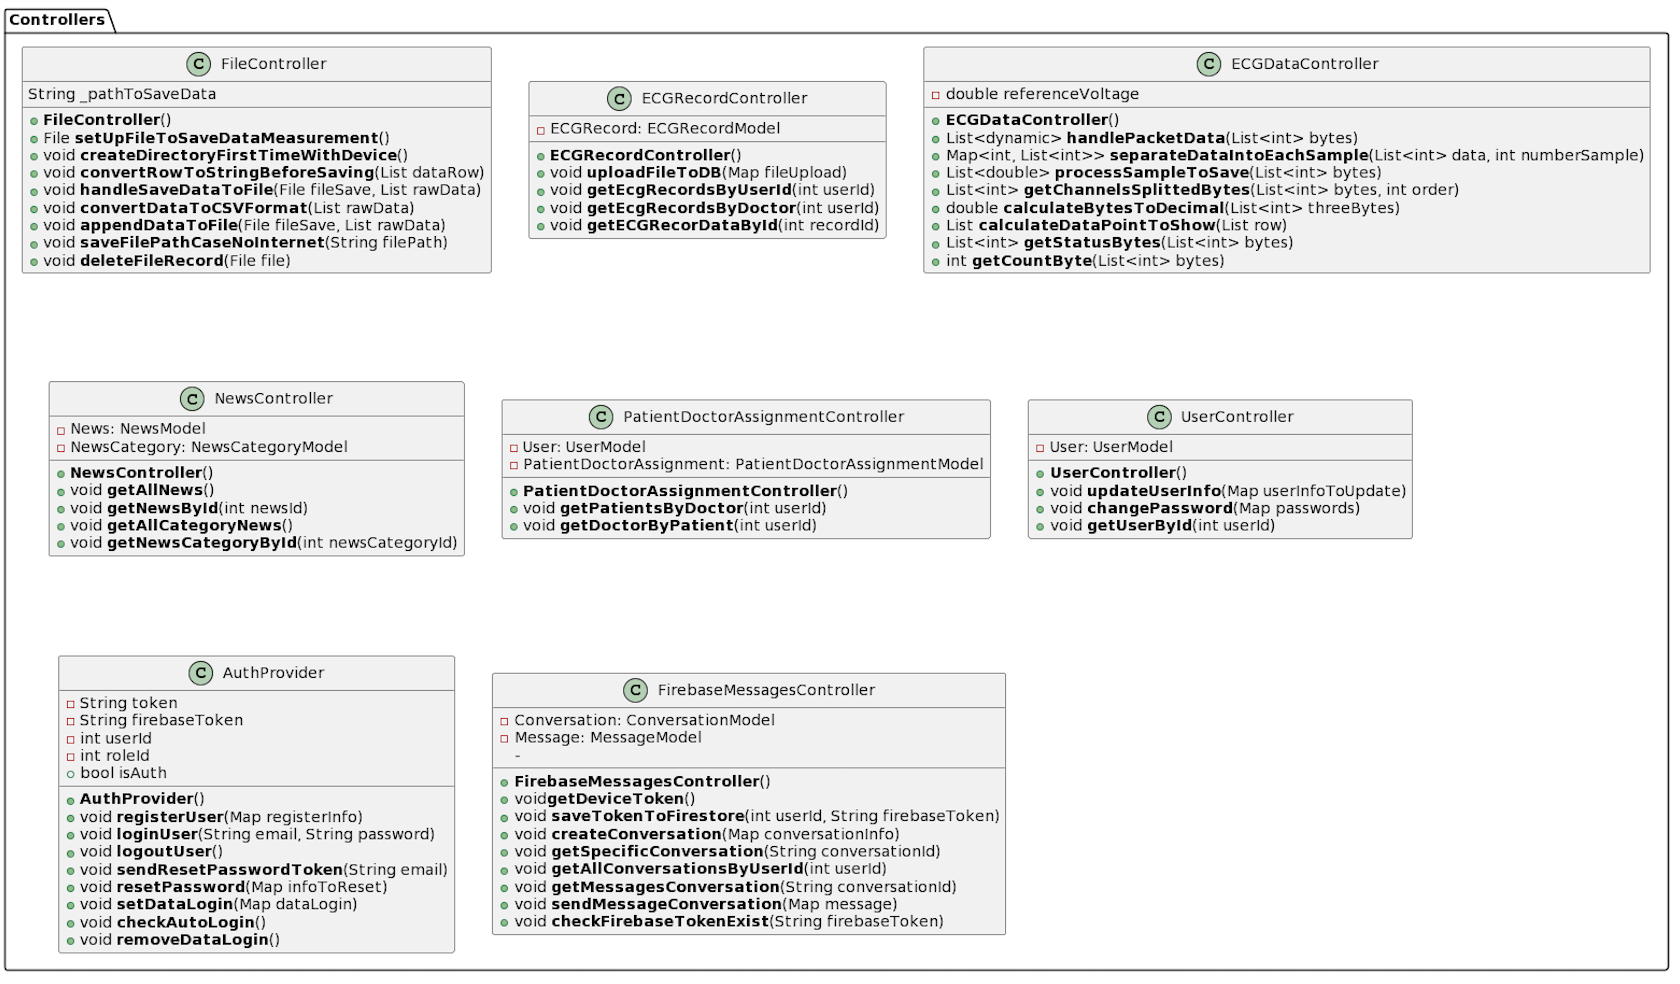
\includegraphics[width=16cm,height=15cm]{Images/mobile_app/class_diagram/mobile_class_controller.png}
    \caption[Sơ đồ lớp của khối Controllers trong ứng dụng di động]{\bfseries \fontsize{12pt}{0pt}\selectfont Sơ đồ lớp của khối Controllers trong ứng dụng di động}
    \label{mobile_class_controller} %đặt tên cho ảnh
  \end{figure}

  Hình \ref{mobile_class_controller} thể hiện các lớp trong Controllers. Mỗi lớp trong Controllers quản lý một nhiệm vụ
  nhất định được chia nhỏ thành các hàm, phương thức tương ứng giúp việc phia chia và đặc biệt khi kiểm soát lỗi rất dễ dàng do
  chúng ta có thể dự đoán được lỗi phát sinh ở chức năng và hàm nào. 

  % //TODO: Thiếu file managements trong sơ đồ
  \begin{itemize}
    \item AuthProvider: Cung cấp các biến và hàm để thực hiện chức năng xác thực người dùng
    \item ECGRecordController: Cung cấp các hàm, phương thức để thực hiện chức năng liên quan đến các bản ghi điện tim
    \item ECGDataController: Cung cấp các hàm, phương thức để xử lý dữ liệu của bản ghi diện tim thời gian thực
    \item FileController: Cung cấp các hàm, phương thức để xử lý file (tạo, sửa, xoá file), phục vụ chính cho ECGRecordController  
    \item NewsController: Cung cấp các hàm, phương thức để lấy dữ liệu tin tức
    \item PatientDoctorAssignmentController: Cung cấp các hàm, phương thức để lấy dữ liệu phân công bệnh nhân/bác sĩ
    \item UserController: Cung cấp các hàm, phương thức để thao tác với dữ liệu người dùng 
    \item FirebaseMessagesController: Cung cấp các hàm, phương thức để thao tác với tin nhắn.
  \end{itemize}

  Các lớp được hình thành là nền tảng để viết code dễ dàng hơn, đồng thời điều này cũng giúp cho cấu trúc thư mục trong
  bất kỳ dự án nào trở nên sạch sẽ và dễ theo dõi hơn.
  
  \end{enumerate}

\paragraph{Server và Website quản trị hệ thống}
\mbox{}

\begin{enumerate}[a)]
\item Danh sách các class diagram

\begin{figure}[H]
  \centering
  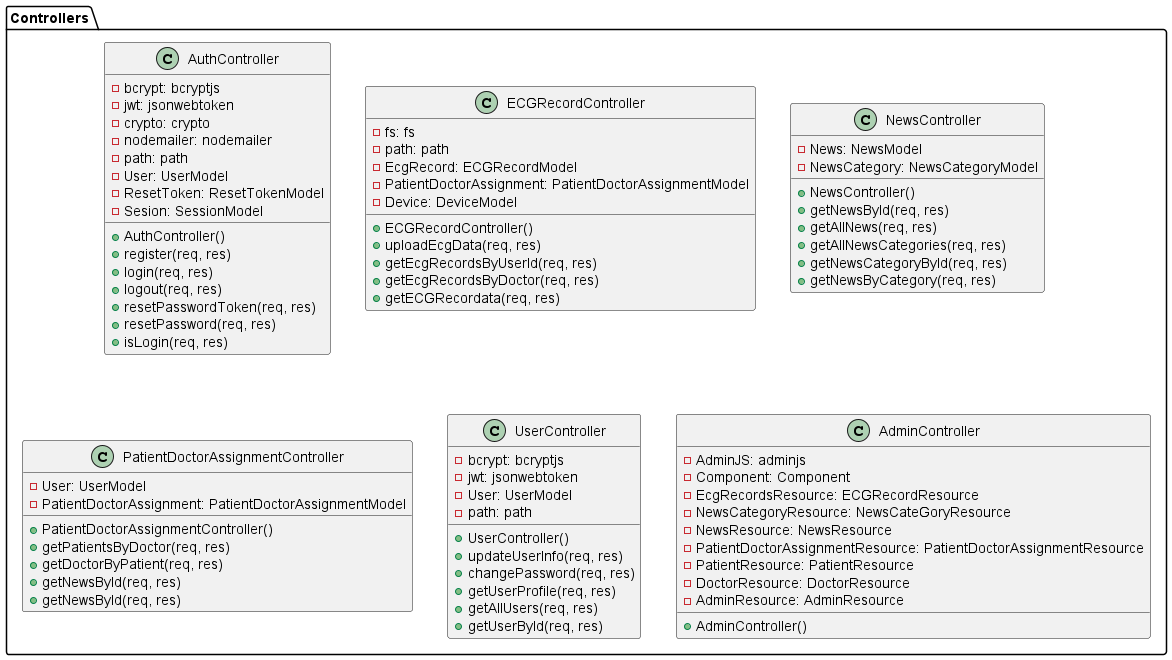
\includegraphics[width=16cm,height=13cm]{Images/server/class/class_controller.png}
  \caption[Sơ đồ lớp của package Controllers]{\bfseries \fontsize{12pt}{0pt}\selectfont Sơ đồ lớp của package Controllers}
  \label{class_controller} %đặt tên cho ảnh
\end{figure}



\begin{figure}[H]
  \centering
  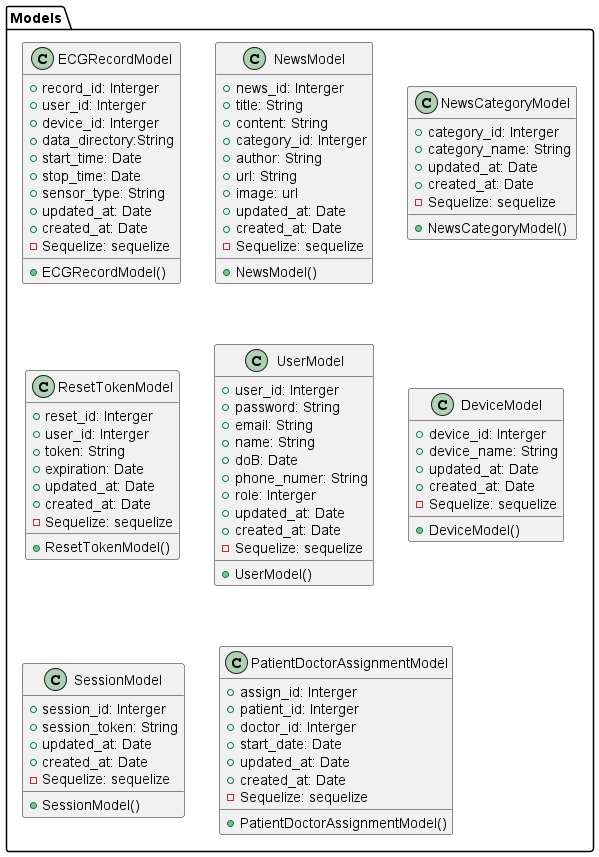
\includegraphics[width=15cm,height=16cm]{Images/server/class/class_model.png}
  \caption[Sơ đồ lớp của package Models]{\bfseries \fontsize{12pt}{0pt}\selectfont Sơ đồ lớp của package Models}
  \label{class_model} %đặt tên cho ảnh
\end{figure}


\begin{figure}[H]
  \centering
  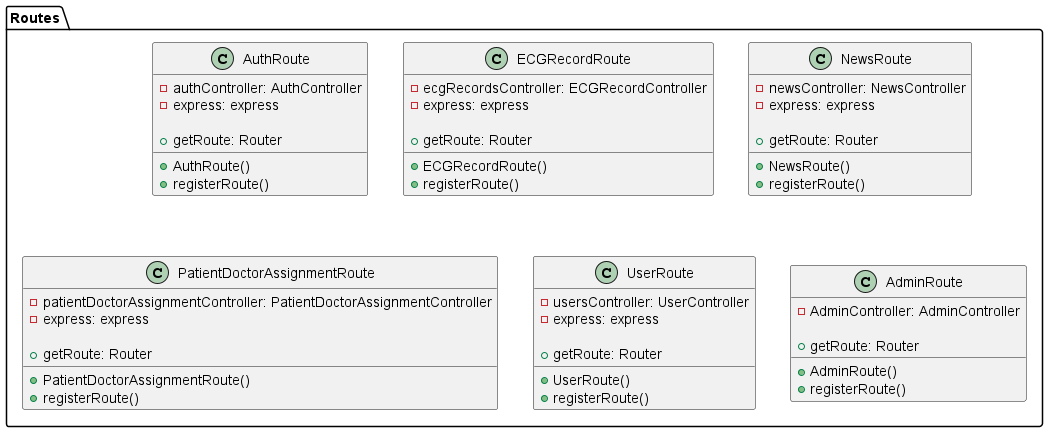
\includegraphics[width=14cm,height=6cm]{Images/server/class/class_route.png}
  \caption[Sơ đồ lớp của package Routes]{\bfseries \fontsize{12pt}{0pt}\selectfont Sơ đồ lớp của package Routes}
  \label{class_route} %đặt tên cho ảnh
\end{figure}


\begin{figure}[H]
  \centering
  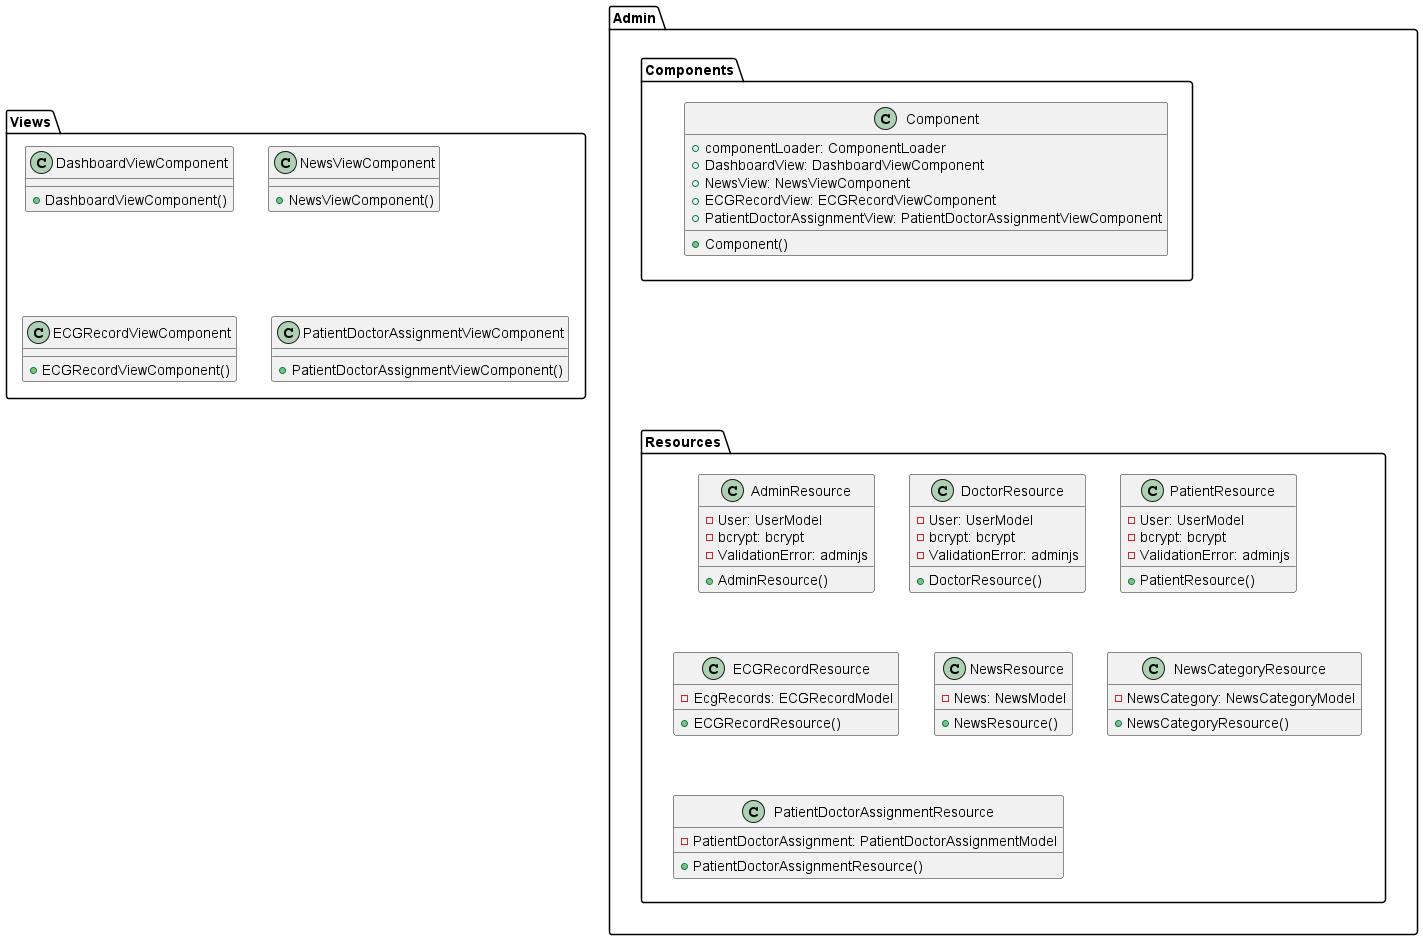
\includegraphics[width=15cm,height=14cm]{Images/server/class/class_admin.png}
  \caption[Sơ đồ lớp của package View và Admin]{\bfseries \fontsize{12pt}{0pt}\selectfont Sơ đồ lớp của package View và Admin}
  \label{class_admin} %đặt tên cho ảnh
\end{figure}


\begin{itemize}

  \item Package "Controllers":

  Chứa các controllers xử lý logic và điều khiển các yêu cầu từ người dùng.
  \item Package "Models":
  
  Chứa các lớp đại diện cho các đối tượng của cơ sở dữ liệu, định nghĩa các thuộc tính và phương thức để làm việc với dữ liệu.
  \item Package "Routes":
  
  Chứa các lớp route, xác định các endpoint và xử lý các yêu cầu HTTP từ người dùng bằng cách gọi tới các controllers tương ứng.
  \item Package "Views":
  
  Chứa các view components đại diện cho giao diện người dùng.
  \item Package "Admin":
  
  Chứa các thành phần liên quan đến trang Admin dashboard.
  \item Package "Resources" (Trong "Admin"):
  
  Chứa các lớp Resource (nguồn tài nguyên) đại diện cho các tài nguyên của trang Admin dashboard, bao gồm: AdminResource, DoctorResource, PatientResource, ECGRecordResource, NewsResource, NewsCategoryResource và PatientDoctorAssignmentResource.
  \item Package "Components" (Trong "Admin"):
  
  Chứa các lớp Components đại diện cho các thành phần giao diện của trang Admin dashboard, bao gồm: ComponentLoader, DashboardViewComponent, NewsViewComponent, ECGRecordViewComponent và PatientDoctorAssignmentViewComponent.
\end{itemize}



\item Mối quan hệ

\begin{figure}[H]
  \centering
  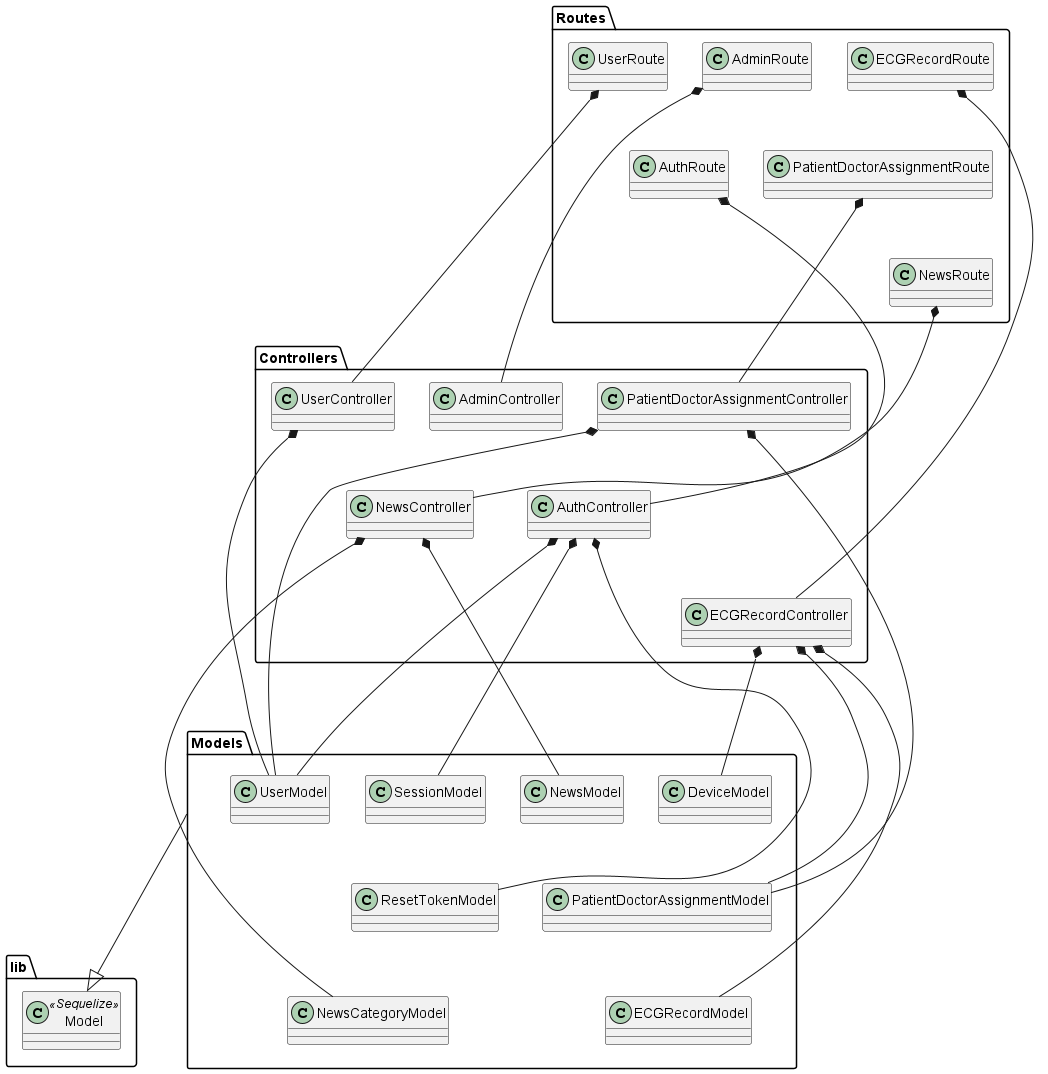
\includegraphics[width=15cm,height=12cm]{Images/server/class/class_relation.png}
  \caption[Mối quan hệ giữa các class ở phía server]{\bfseries \fontsize{12pt}{0pt}\selectfont Mối quan hệ giữa các class ở phía server}
  \label{class_relation} %đặt tên cho ảnh
\end{figure}


\begin{figure}[H]
  \centering
  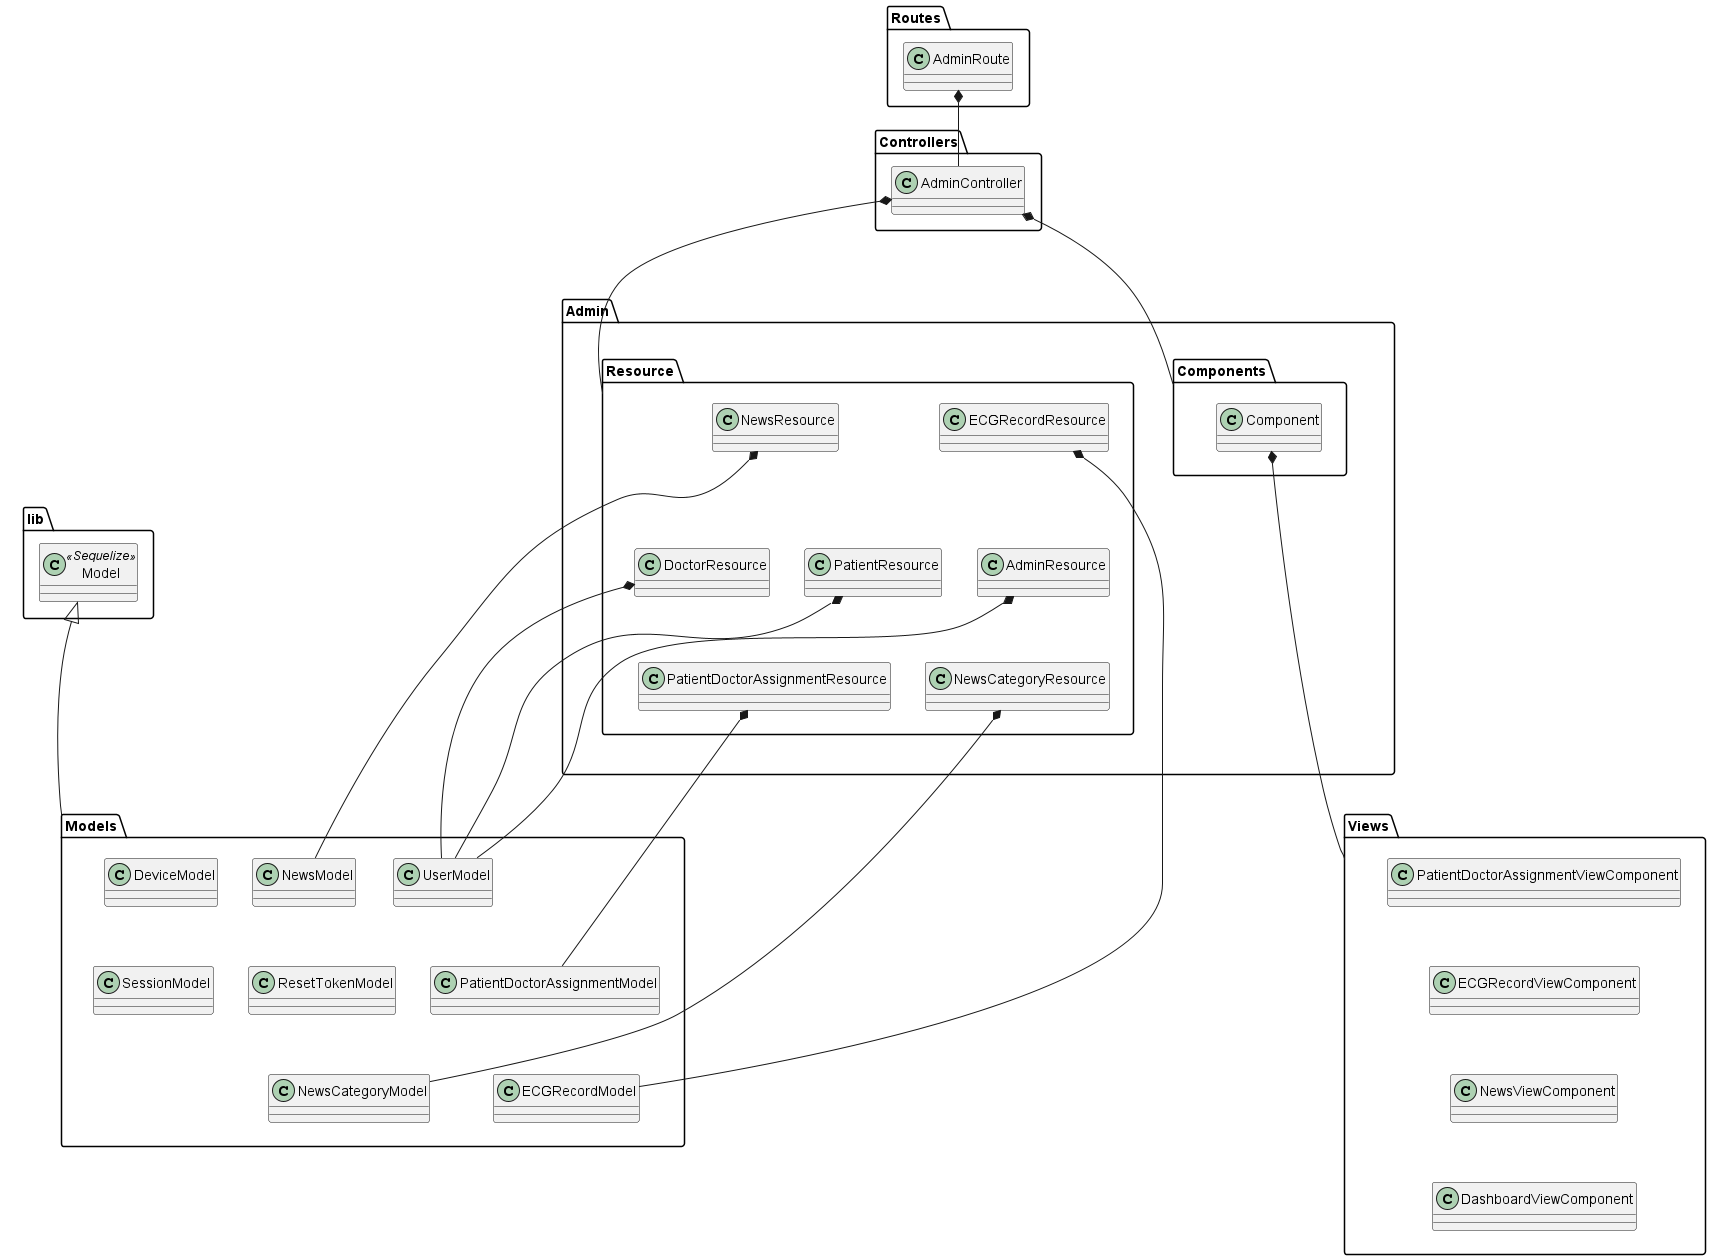
\includegraphics[width=16cm,height=15cm]{Images/server/class/class_admin_relation.png}
  \caption[Mối quan hệ giữa các class ở phía website quản trị]{\bfseries \fontsize{12pt}{0pt}\selectfont Mối quan hệ giữa các class ở phía website quản trị}
  \label{class_admin_relation} %đặt tên cho ảnh
\end{figure}

\end{enumerate}



\subsubsection{Thiết kế giao diện}

\paragraph{Ứng dụng}
\mbox{}

Dưới đây là các giao diện thực tế mà chúng em thiết kế cho App:
\begin{figure}[H]
  \centering
  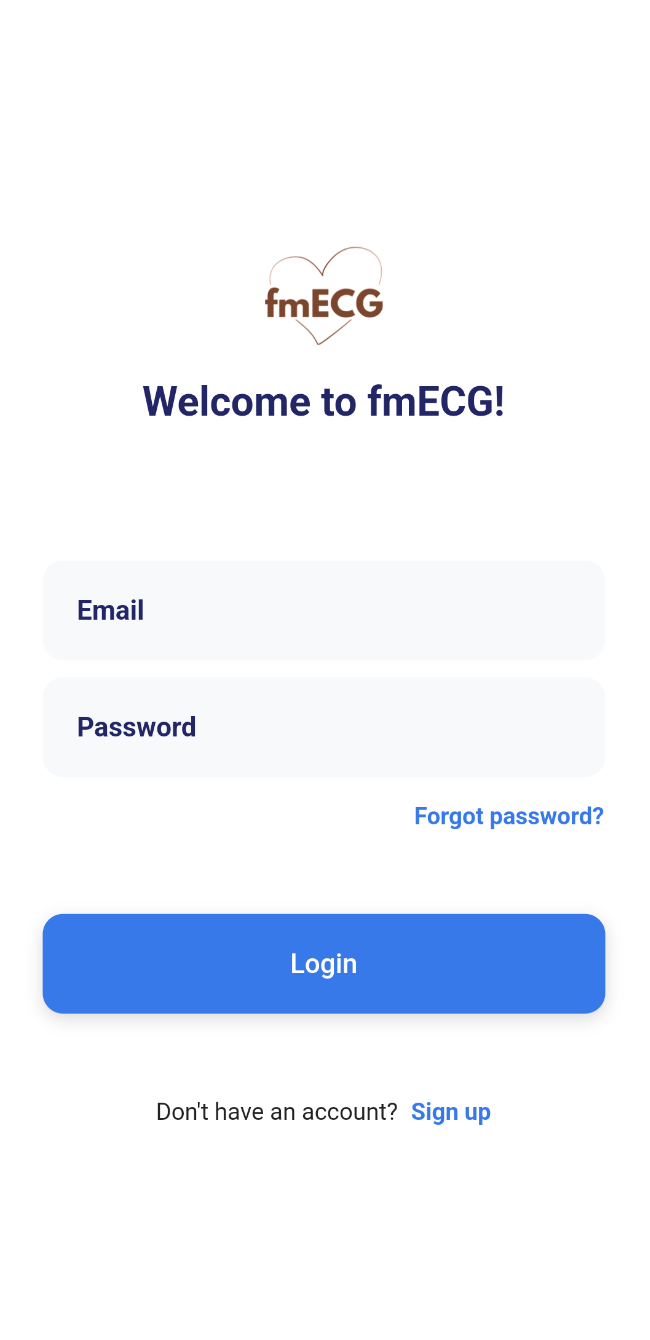
\includegraphics[width=6cm,height=12cm]{Images/mobile_app/demo/login.png}
  \caption[Giao diện trang đăng nhập]{\bfseries \fontsize{12pt}{0pt}\selectfont Giao diện trang đăng nhập}
  \label{demo_login} %đặt tên cho ảnh
\end{figure}

Trang đăng nhập gồm có logo, sau đó là hai ô để nhập email và mật khẩu, cùng một nút màu xanh cho người dùng nhấn để kiểm tra 
việc đăng nhập vào
trang chủ nếu email và mật khẩu của người dùng được xác thực. Nếu việc xác thực không thành công, giao diện sẽ hiển thị
một dòng chữ dưới hai ô nhập.

Ngoài ra nếu người dùng chưa có tài khoản thì có thể chọn đăng ký ở dưới để chuyển sang trang đăng ký.

\begin{figure}[H]
  \centering
  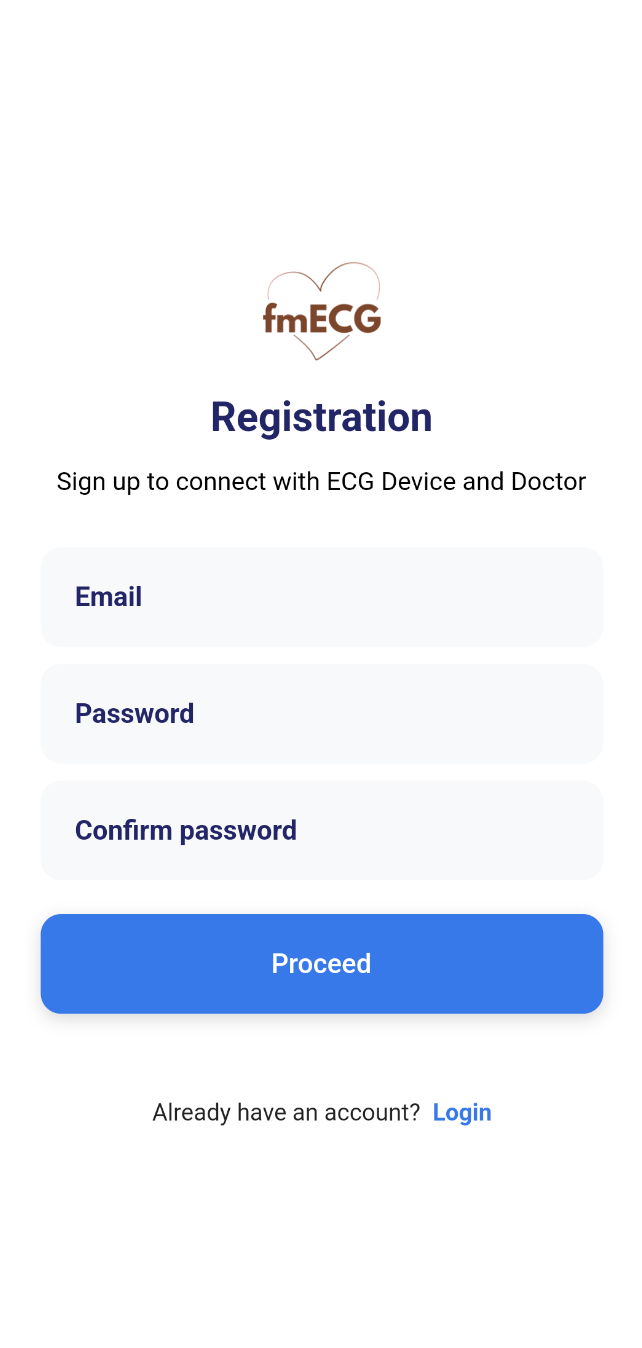
\includegraphics[width=6cm,height=12cm]{Images/mobile_app/demo/register.png}
  \caption[Giao diện trang đăng ký tài khoản]{\bfseries \fontsize{12pt}{0pt}\selectfont Giao diện trang đăng ký tài khoản}
  \label{demo_register} %đặt tên cho ảnh
\end{figure}

Trang đăng ký gồm có 3 ô để người dùng đăng ký tài khoản một cách nhanh chóng

\begin{figure}[H]
  \centering
  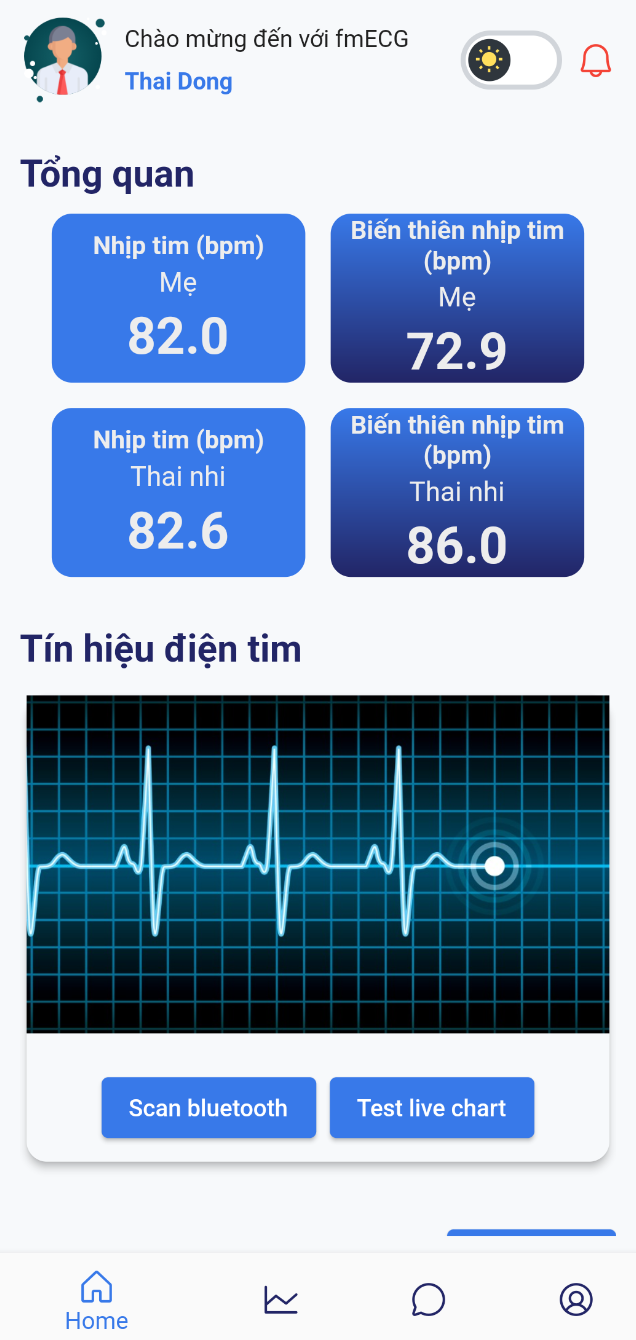
\includegraphics[width=6cm,height=12cm]{Images/mobile_app/demo/home_screen.png}
  \caption[Giao diện trang]{\bfseries \fontsize{12pt}{0pt}\selectfont Giao diện trang}
  \label{demo_} %đặt tên cho ảnh
\end{figure}

\begin{figure}[H]
  \centering
  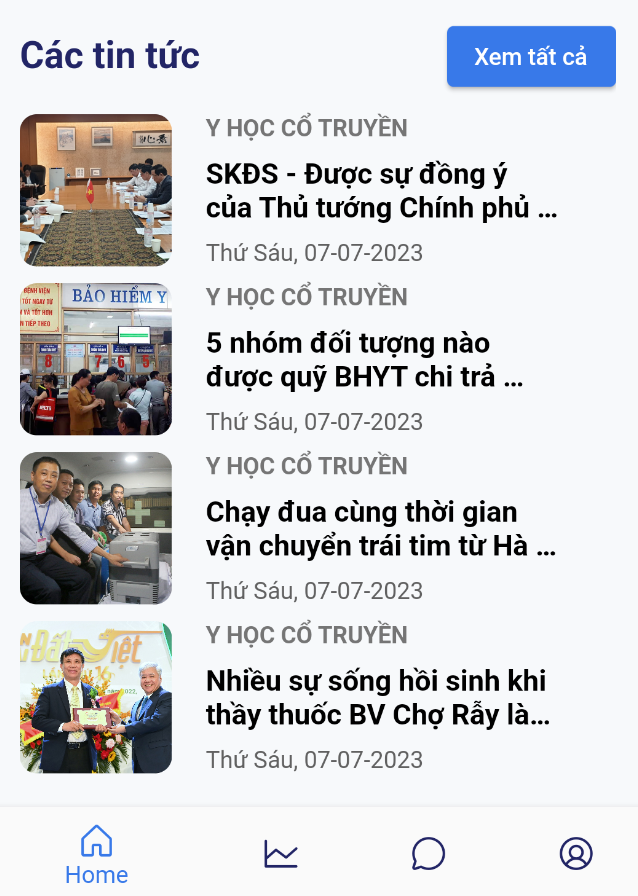
\includegraphics[width=6cm,height=8cm]{Images/mobile_app/demo/preview_news.png}
  \caption[Giao diện trang]{\bfseries \fontsize{12pt}{0pt}\selectfont Giao diện trang}
  \label{demo_} %đặt tên cho ảnh
\end{figure}

\begin{figure}[H]
  \centering
  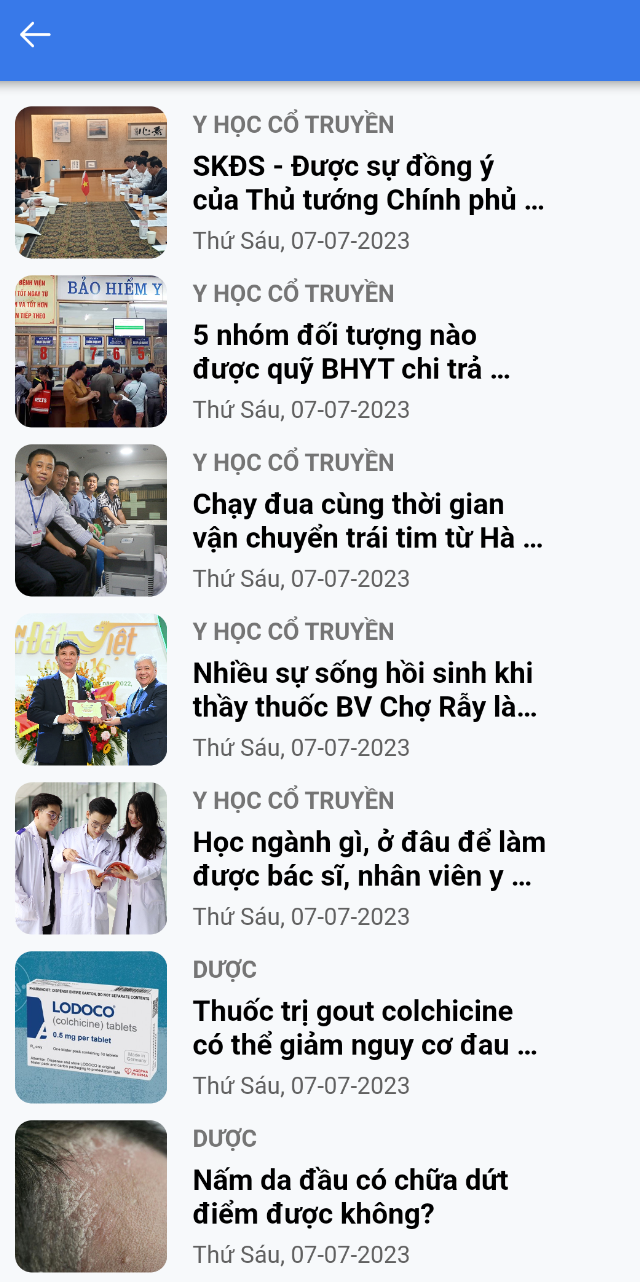
\includegraphics[width=6cm,height=12cm]{Images/mobile_app/demo/all_news.png}
  \caption[Giao diện trang]{\bfseries \fontsize{12pt}{0pt}\selectfont Giao diện trang}
  \label{demo_} %đặt tên cho ảnh
\end{figure}

\begin{figure}[H]
  \centering
  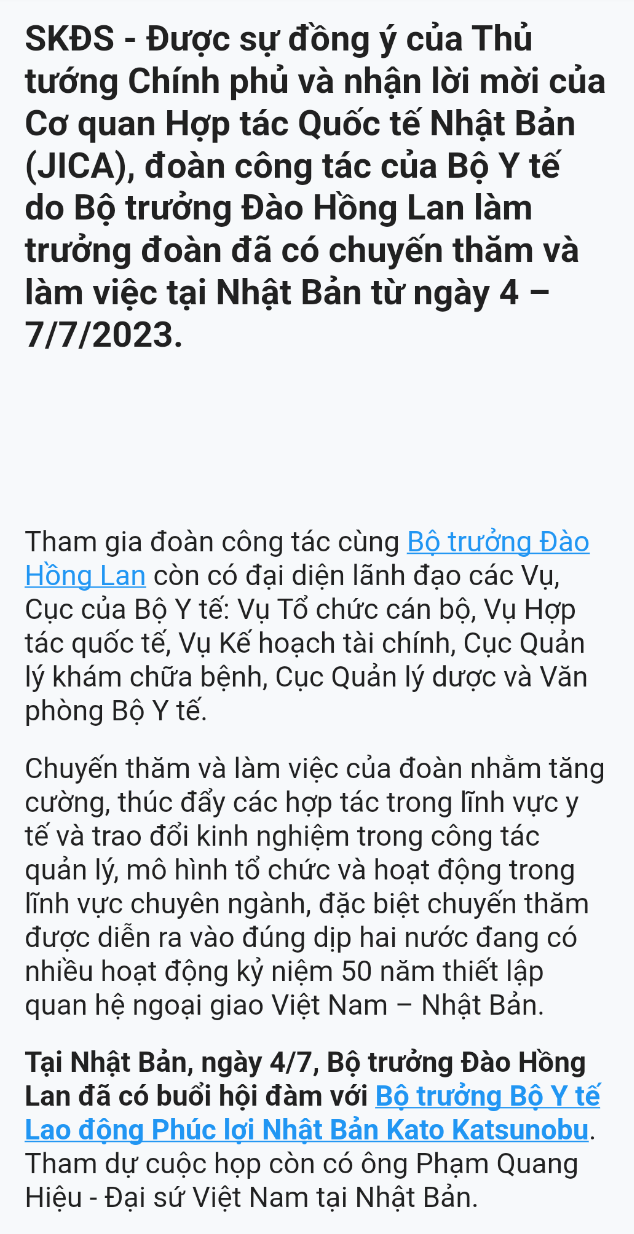
\includegraphics[width=6cm,height=12cm]{Images/mobile_app/demo/detail_news.png}
  \caption[Giao diện trang]{\bfseries \fontsize{12pt}{0pt}\selectfont Giao diện trang}
  \label{demo_} %đặt tên cho ảnh
\end{figure}

\begin{figure}[H]
  \centering
  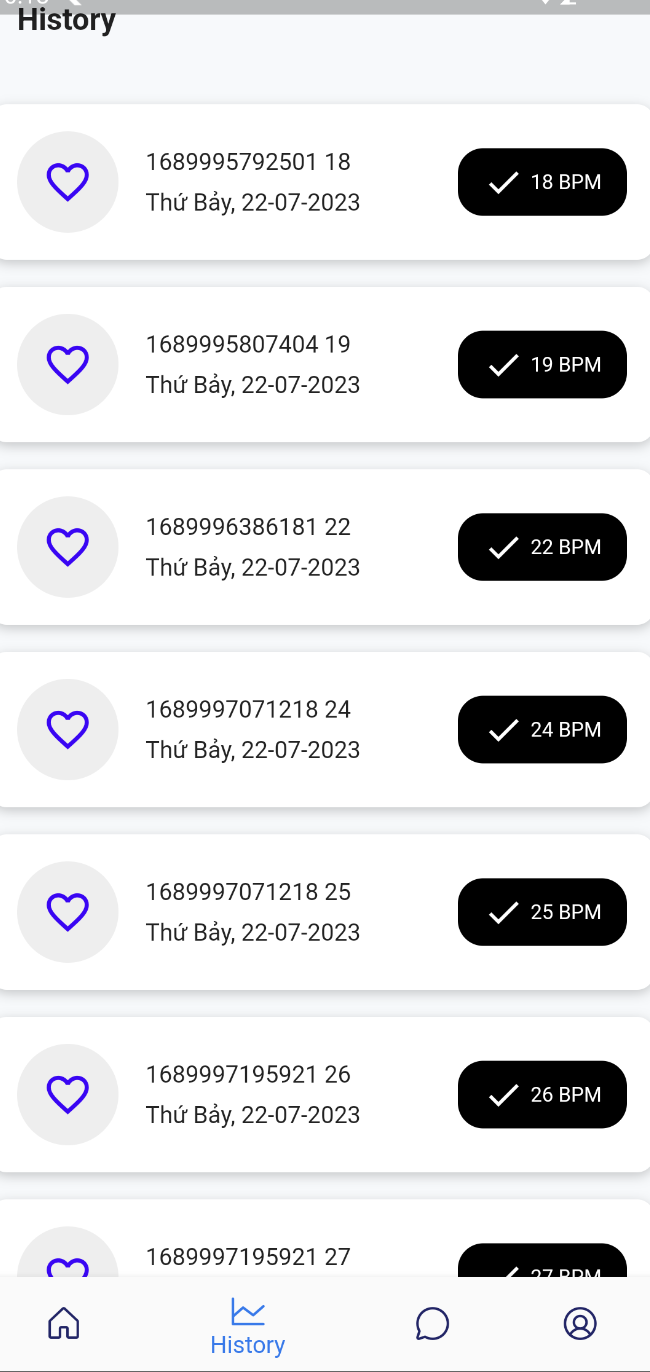
\includegraphics[width=6cm,height=12cm]{Images/mobile_app/demo/history.png}
  \caption[Giao diện trang]{\bfseries \fontsize{12pt}{0pt}\selectfont Giao diện trang}
  \label{demo_} %đặt tên cho ảnh
\end{figure}

\begin{figure}[H]
  \centering
  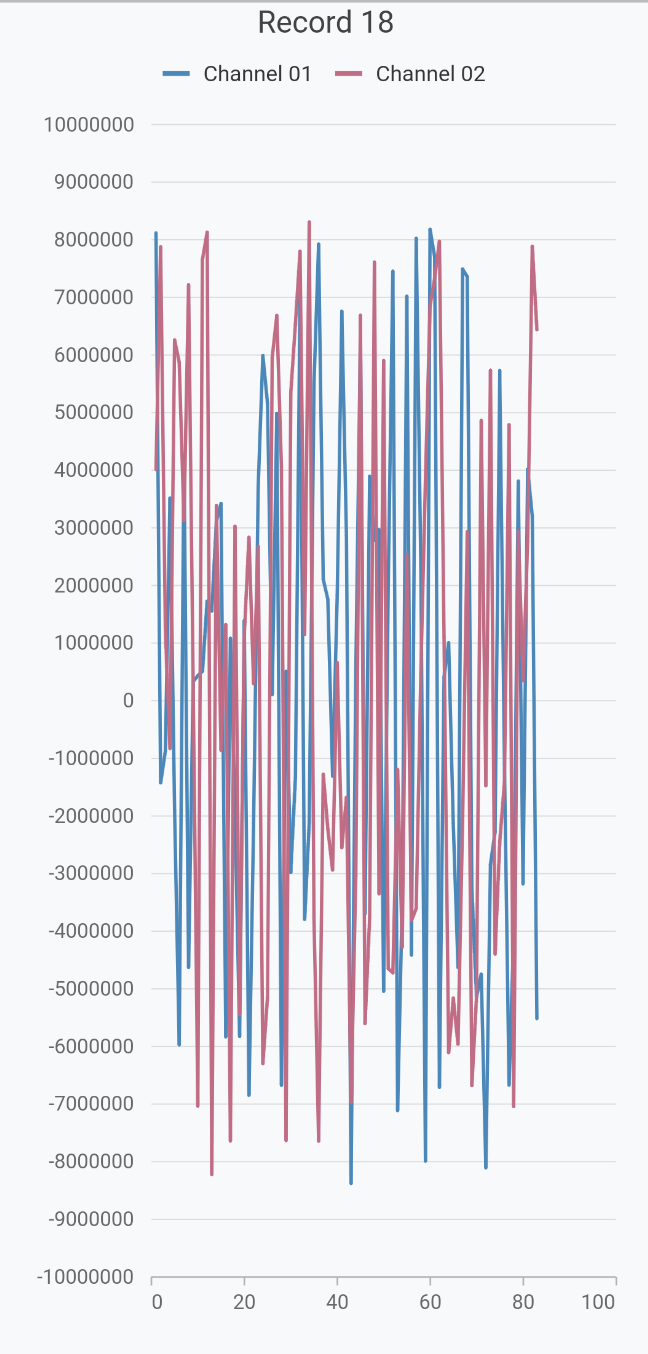
\includegraphics[width=6cm,height=12cm]{Images/mobile_app/demo/detail_record.png}
  \caption[Giao diện trang]{\bfseries \fontsize{12pt}{0pt}\selectfont Giao diện trang}
  \label{demo_} %đặt tên cho ảnh
\end{figure}

\begin{figure}[H]
  \centering
  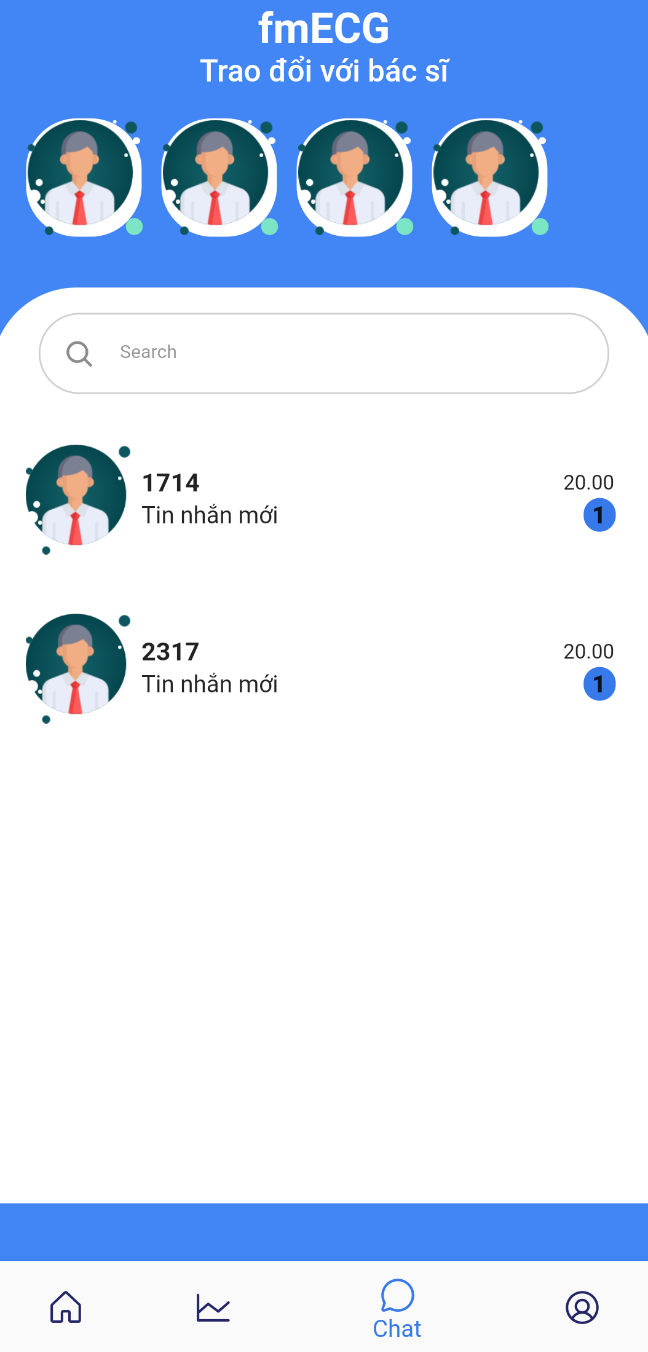
\includegraphics[width=6cm,height=12cm]{Images/mobile_app/demo/chat_preview.png}
  \caption[Giao diện trang]{\bfseries \fontsize{12pt}{0pt}\selectfont Giao diện trang}
  \label{demo_} %đặt tên cho ảnh
\end{figure}

\begin{figure}[H]
  \centering
  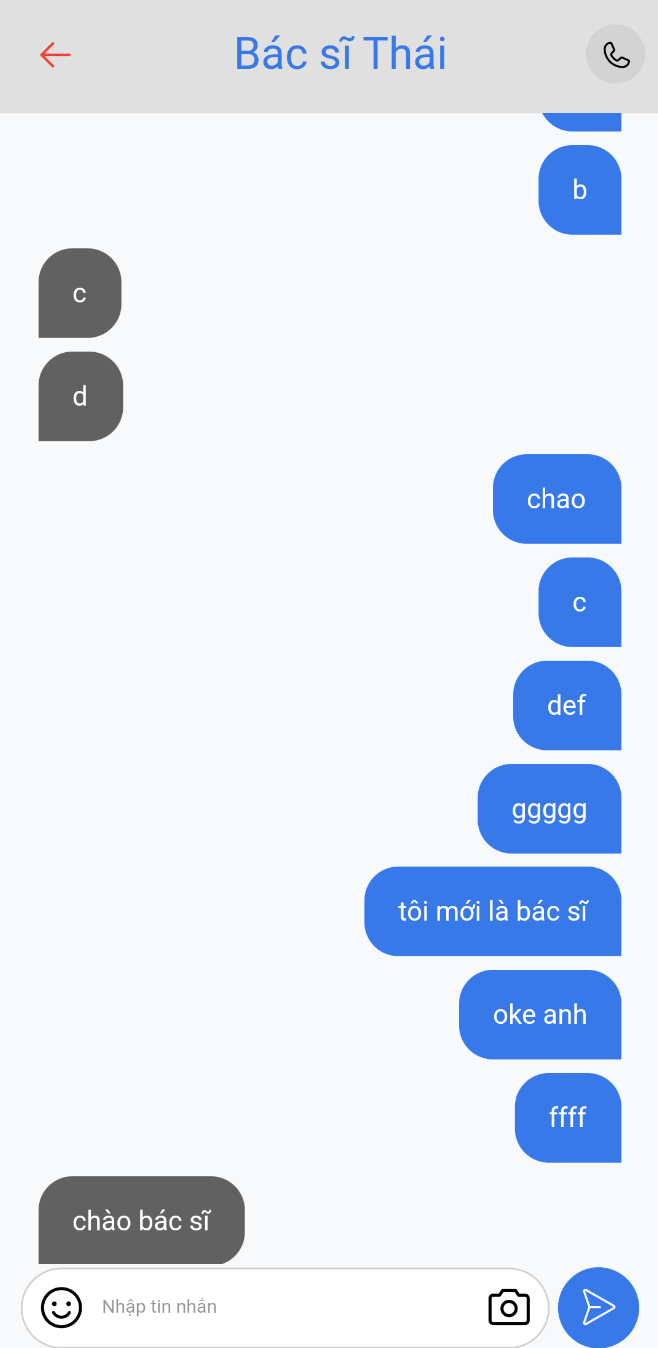
\includegraphics[width=6cm,height=12cm]{Images/mobile_app/demo/chat_detail.png}
  \caption[Giao diện trang]{\bfseries \fontsize{12pt}{0pt}\selectfont Giao diện trang}
  \label{demo_} %đặt tên cho ảnh
\end{figure}

\begin{figure}[H]
  \centering
  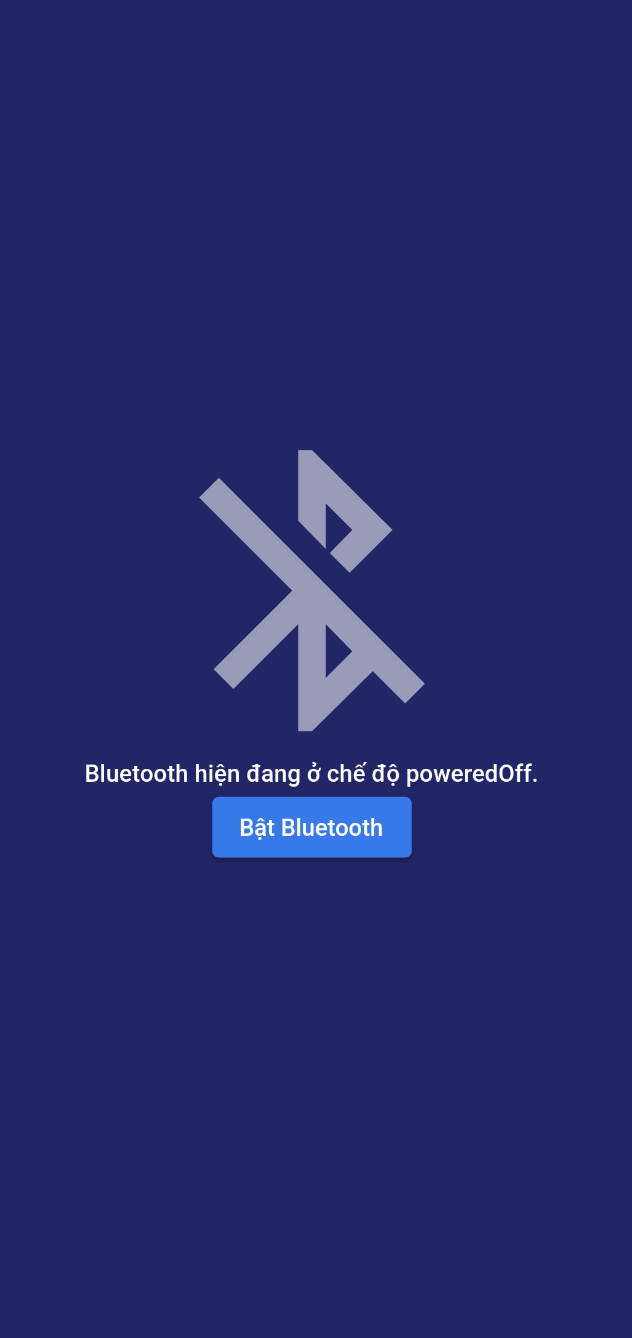
\includegraphics[width=6cm,height=12cm]{Images/mobile_app/demo/off_bluetooth.png}
  \caption[Giao diện trang]{\bfseries \fontsize{12pt}{0pt}\selectfont Giao diện trang}
  \label{demo_} %đặt tên cho ảnh
\end{figure}

\begin{figure}[H]
  \centering
  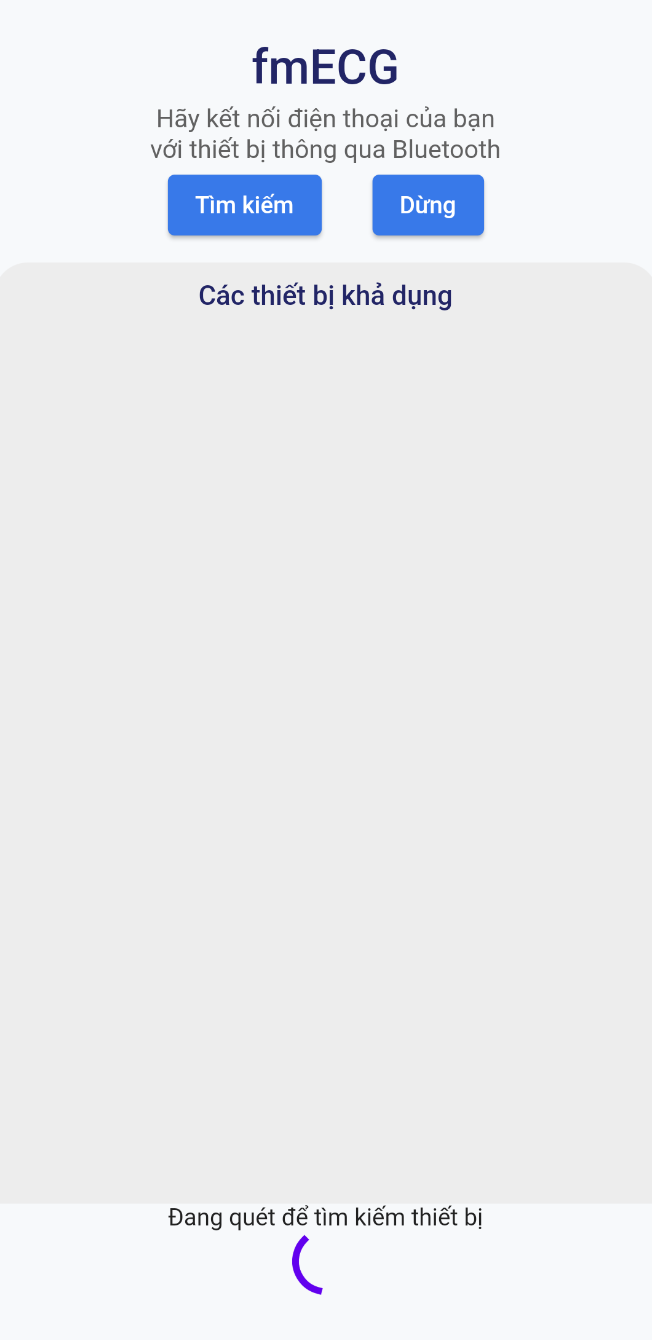
\includegraphics[width=6cm,height=12cm]{Images/mobile_app/demo/finding_bluetooth.png}
  \caption[Giao diện trang]{\bfseries \fontsize{12pt}{0pt}\selectfont Giao diện trang}
  \label{demo_} %đặt tên cho ảnh
\end{figure}



\paragraph{Website}
\mbox{}

\subsubsection{Thiết kế các chức năng cho Website và Server}
\subsubsection{Thiết kế API}

\paragraph{API liên quan đến thông tin người dùng}
\mbox{}

\begin{table}[H]
     \centering
     \caption{\bfseries \fontsize{12pt}{0pt}\selectfont Bảng API liên quan đến thông tin người dùng}
     \begin{tabularx}{0.9\textwidth}{
     | >{\raggedright\arraybackslash}X
     | >{\raggedright\arraybackslash}m{2cm}
     | >{\raggedright\arraybackslash}X|
     }
     \hline
     \bfseries Đường dẫn    &\bfseries Phương thức    &\bfseries Mô tả\\ \hline
    api/users/profile   &   GET  &  Lấy thông tin của người dùng với đầu vào là JWT token khi người dùng đăng nhập thành công vào hệ thống \\  \hline
    api/users/profile   &    PUT    &  Cập nhật thông tin người dùng \\  \hline
    api/users/change-password   &   PUT     & Thay đổi mật khẩu của người dùng  \\ \hline
    api/users/\{:userId\}  &   GET     & Lấy thông tin của người dùng cụ thể theo user id \\ \hline

     \end{tabularx}
     \label{table_api_user}
\end{table}



\paragraph{API liên quan đến việc xác thực người dùng }
\mbox{}

\begin{table}[H]
  \centering
  \caption{\bfseries \fontsize{12pt}{0pt}\selectfont Bảng API liên quan đến việc xác thực người dùng}
  \begin{tabularx}{0.9\textwidth}{
  | >{\raggedright\arraybackslash}X
  | >{\raggedright\arraybackslash}m{2cm}
  | >{\raggedright\arraybackslash}X|
  }
  \hline
  \bfseries Đường dẫn    &\bfseries Phương thức    &\bfseries Mô tả\\ \hline
 api/register   &   POST  & Đăng ký tài khoản \\ \hline
 api/login   &    POST    & Đăng nhập vào hệ thống \\ \hline
 api/logout  &   GET     & Đăng xuất khỏi hệ thống \\ \hline
 api/reset-password  &     POST   &  Gửi reset token đến email của người dùng để reset mật khẩu \\  \hline
 api/reset-password/reset &   POST     & Giúp reset lại mật khẩu mới với verify token được nhận từ api: api/reset-password  \\ \hline

  \end{tabularx}
  \label{table_api_auth}
\end{table}



\paragraph{API liên quan đến tin tức}
\mbox{}

\begin{table}[H]
  \centering
  \caption{\bfseries \fontsize{12pt}{0pt}\selectfont Bảng API liên quan đến tin tức}
  \begin{tabularx}{0.9\textwidth}{
  | >{\raggedright\arraybackslash}X
  | >{\raggedright\arraybackslash}m{2cm}
  | >{\raggedright\arraybackslash}X|
  }
  \hline
  \bfseries Đường dẫn    &\bfseries Phương thức    &\bfseries Mô tả\\ \hline
 api/news/\{:newsId\}   &   GET  & Lấy nội của tin tức tương ứng với id dưới dạng HTML \\ \hline
 api/news   &    GET    & Lấy toàn bộ danh sách thông tin của tin tức \\ \hline
 api/categories  &   GET     & Lấy toàn bộ danh sách thông tin của tin tức \\ \hline
 api/category/\{:categoryId\}   &     GET   & Lấy thông tin của loại tin tức theo id tương ứng \\ \hline
 api/ news/category/\{:categoryId\} &   GET     & Lấy toàn bộ thông tin của tin tức theo id của loại tin \\ \hline

  \end{tabularx}
  \label{table_api_news}
\end{table}

\paragraph{API liên quan đến bản ghi ECG}
\mbox{}

\begin{table}[H]
  \centering
  \caption{\bfseries \fontsize{12pt}{0pt}\selectfont Bảng API liên quan đến bản ghi ECG}
  \begin{tabularx}{0.9\textwidth}{
  | >{\raggedright\arraybackslash}X
  | >{\raggedright\arraybackslash}m{2cm}
  | >{\raggedright\arraybackslash}X|
  }
  \hline
  \bfseries Đường dẫn    &\bfseries Phương thức    &\bfseries Mô tả\\ \hline
 api/ecg-records/upload   &   POST  & Tải dữ liệu của phiên đo ECG lên server \\ \hline
 api/ecg-records/patient/\{:patientId\}   &    GET    & Lấy danh sách thông tin các phiên đo ECG của bệnh nhân \\ \hline
 api/ecg-records/doctor/\{:doctorId\} &   GET     & Lấy danh sách thông tin các phiên đo ECG của các bệnh nhân được quản lý bởi bác sỹ \\ \hline
 api/ecg-records/record-data/\{:recordId\}  &     GET   & Lấy dữ liệu một phiên đo của bệnh nhân \\ \hline

  \end{tabularx}
  \label{table_api_ecg}
\end{table}



\paragraph{API liên quan liên quan đến việc phân công bệnh nhân cho bác sỹ}
\mbox{}

\begin{table}[H]
  \centering
  \caption{\bfseries \fontsize{12pt}{0pt}\selectfont Bảng API liên quan liên quan đến việc phân công bệnh nhân cho bác sỹ}
  \begin{tabularx}{0.9\textwidth}{
  | >{\raggedright\arraybackslash}X
  | >{\raggedright\arraybackslash}m{2cm}
  | >{\raggedright\arraybackslash}X|
  }
  \hline
  \bfseries Đường dẫn    &\bfseries Phương thức    &\bfseries Mô tả\\ \hline
   api/doctor/\{:doctorId\}/patients   &   GET  & Lấy danh sách thông tin bệnh nhân được phân công cho bác sĩ \\ \hline
  api/patient/\{:patientId\}/doctor  &    GET    & Lấy thông tin bác sỹ được phân công cho bệnh nhân \\ \hline

  \end{tabularx}
  \label{table_api_pat_doc}
\end{table}


\subsubsection{Sơ đồ tuần tự}

% ------------------------User----------------------

\paragraph{API liên quan đến thông tin người dùng}
\mbox{}


% sửa lại ảnh 
\begin{figure}[H]
  \centering
  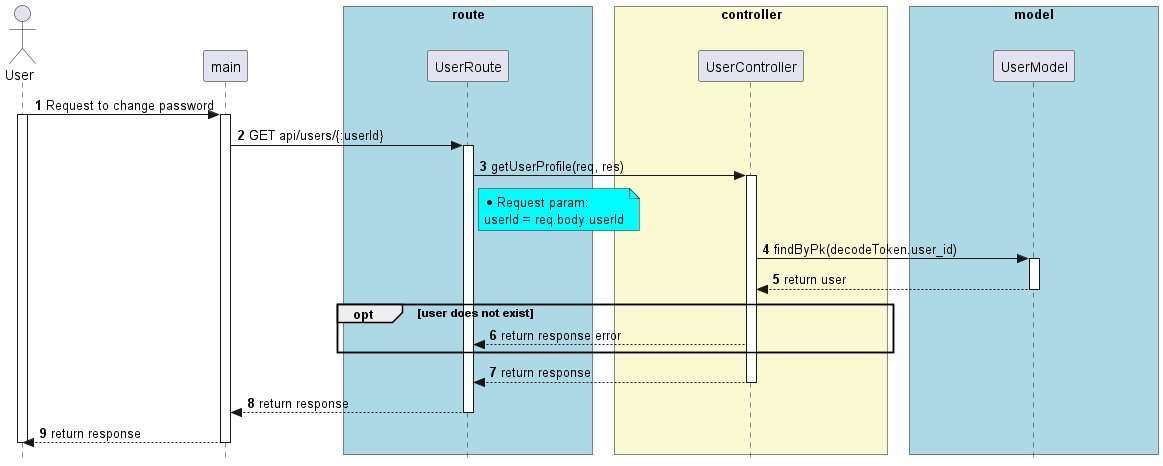
\includegraphics[width=16cm,height=9cm]{Images/server/sequence/server/getUserById.png}
  \caption[Sơ đồ tuần tự cho API lấy thông tin của người dùng dựa trên ID ]{\bfseries \fontsize{12pt}{0pt}
  \selectfont Sơ đồ tuần tự cho API lấy thông tin của người dùng dựa trên ID }
  \label{getUserById} %đặt tên cho ảnh
\end{figure}
Hình \ref{getUserById} mô tả quá trình lấy thông tin người dùng dựa trên ID trong ứng dụng. Người dùng gửi yêu cầu lấy thông tin người dùng theo ID, thông qua các tầng của hệ thống, yêu cầu này được xử lý bởi UserController. UserController kiểm tra thông tin và truy vấn UserModel để lấy thông tin người dùng. Nếu người dùng không tồn tại, hệ thống trả về response lỗi, ngược lại, response chứa thông tin người dùng được gửi lại từ UserController tới người dùng.


% sửa lại ảnh 
\begin{figure}[H]
  \centering
  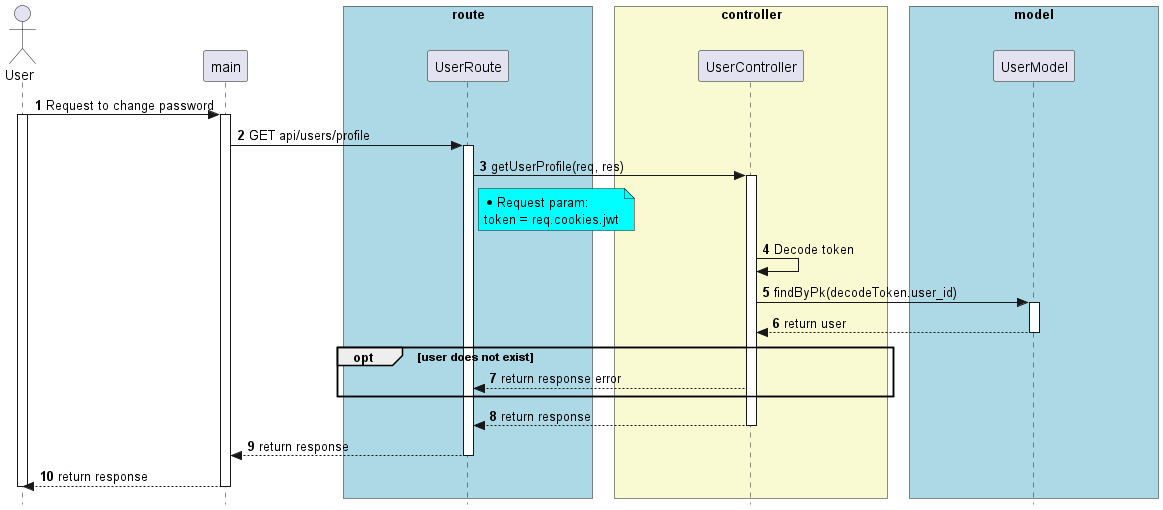
\includegraphics[width=16cm,height=9cm]{Images/server/sequence/server/getUserProfile.png}
  \caption[Sơ đồ tuần tự cho API lấy thông tin của người dùng dựa trên JWT token ]{\bfseries \fontsize{12pt}{0pt}
  \selectfont Sơ đồ tuần tự cho API lấy thông tin của người dùng dựa trên JWT token }
  \label{getUserProfile} %đặt tên cho ảnh
\end{figure}
Hình \ref{getUserProfile} mô tả quá trình lấy thông tin hồ sơ người dùng trong ứng dụng. Người dùng gửi yêu cầu lấy thông tin hồ sơ, thông qua các tầng của hệ thống, yêu cầu này được xử lý bởi UserController. UserController giải mã mã thông báo (token) để xác định người dùng, sau đó truy vấn UserModel để lấy thông tin hồ sơ của người dùng dựa trên user\_id từ mã giải mã. Nếu người dùng không tồn tại, hệ thống trả về response lỗi, ngược lại, response chứa thông tin hồ sơ của người dùng được gửi lại từ UserController tới người dùng.




% \linebreak


\begin{figure}[H]
  \centering
  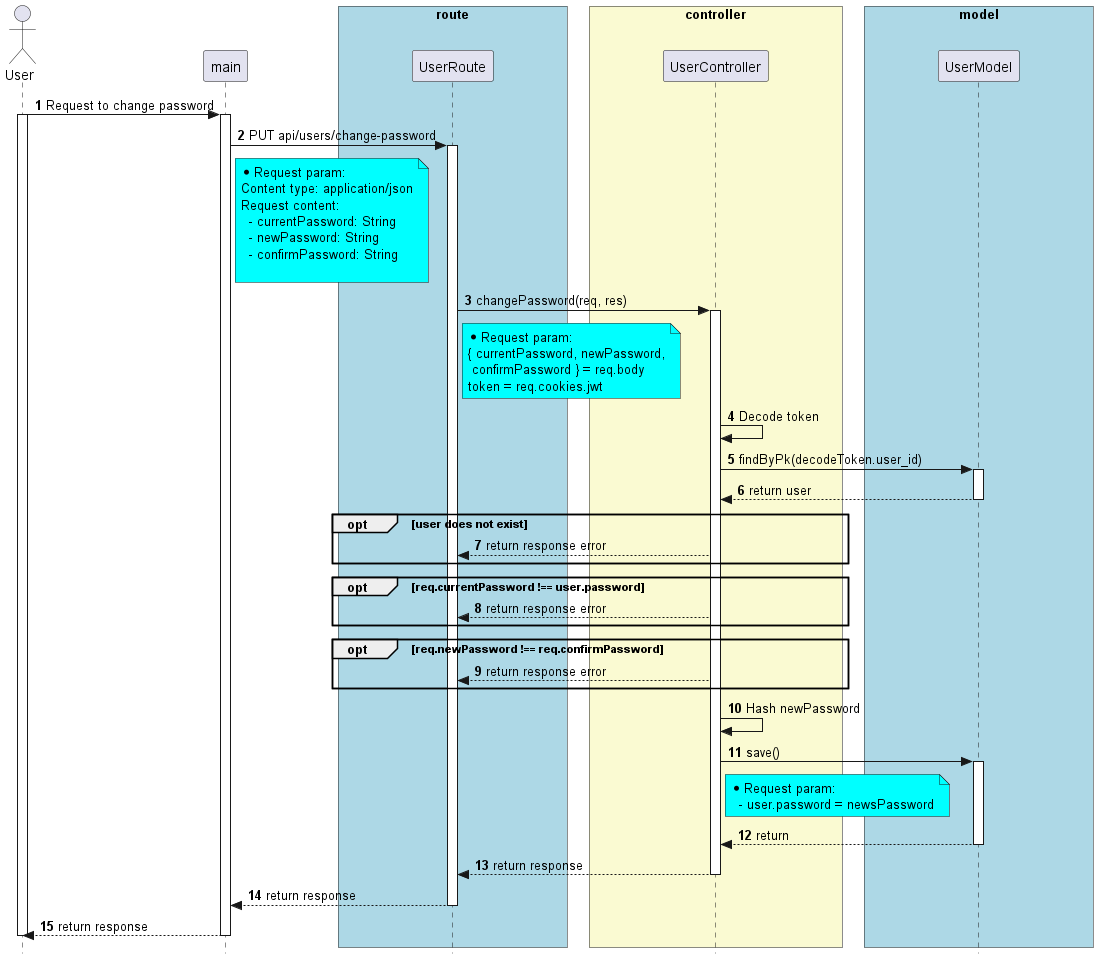
\includegraphics[width=14cm,height=15cm]{Images/server/sequence/server/changePassword.png}
  \caption[Sơ đồ tuần tự cho API thay đổi mật khẩu người dùng ]{\bfseries \fontsize{12pt}{0pt}
  \selectfont Sơ đồ tuần tự cho API thay đổi mật khẩu người dùng }
  \label{changePassword} %đặt tên cho ảnh
\end{figure}

Hình \ref{changePassword} mô tả quá trình thay đổi mật khẩu người dùng trong ứng dụng. Người dùng gửi yêu cầu thay đổi mật khẩu, thông qua các tầng của hệ thống, yêu cầu này được xử lý bởi UserController. Đầu tiên, hệ thống sẽ kiểm tra và giải mã mã thông báo (token) để xác định người dùng. Sau đó, UserController truy vấn UserModel để tìm người dùng dựa trên user\_id từ mã giải mã. Nếu người dùng không tồn tại hoặc mật khẩu hiện tại không khớp với mật khẩu trong hệ thống, hoặc mật khẩu mới không khớp với xác nhận mật khẩu, hệ thống sẽ trả về response lỗi tương ứng. Ngược lại, mật khẩu mới sẽ được mã hóa và lưu vào UserModel, sau đó hệ thống trả về response thành công tới người dùng.



\begin{figure}[H]
  \centering
  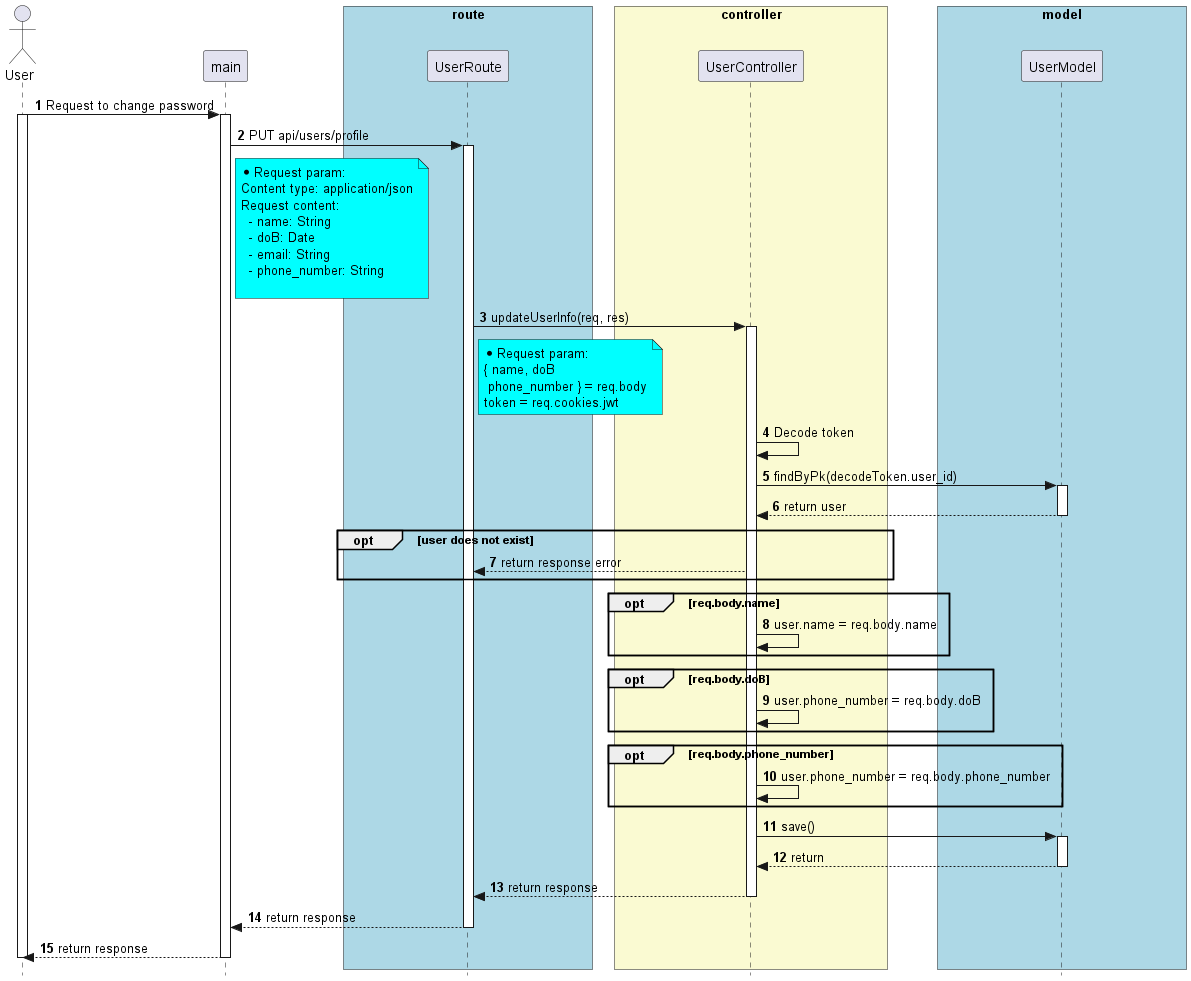
\includegraphics[width=16cm,height=12cm]{Images/server/sequence/server/updateUserInfo.png}
  \caption[Sơ đồ tuần tự cho API cập nhật thông tin người dùng ]{\bfseries \fontsize{12pt}{0pt}
  \selectfont Sơ đồ tuần tự cho API cập nhật thông tin người dùng }
  \label{updateUserInfo} %đặt tên cho ảnh
\end{figure}

Hình \ref{updateUserInfo} mô tả quá trình cập nhật thông tin người dùng trong ứng dụng. Người dùng gửi yêu cầu cập nhật thông tin, thông qua các tầng của hệ thống, yêu cầu này được xử lý bởi UserController. Đầu tiên, hệ thống sẽ kiểm tra và giải mã mã thông báo (token) để xác định người dùng. Sau đó, UserController truy vấn UserModel để tìm người dùng dựa trên user\_id từ mã giải mã. Nếu người dùng không tồn tại, hệ thống sẽ trả về response lỗi. Ngược lại, thông tin cập nhật như tên, ngày sinh (dob), và số điện thoại (phone\_number) sẽ được cập nhật vào UserModel. Sau đó, hệ thống trả về response thành công tới người dùng.


% ----------------------------------------------



% ------------------------Auth----------------------

\paragraph{API liên quan đến việc xác thực người dùng }
\mbox{}


\begin{figure}[H]
  \centering
  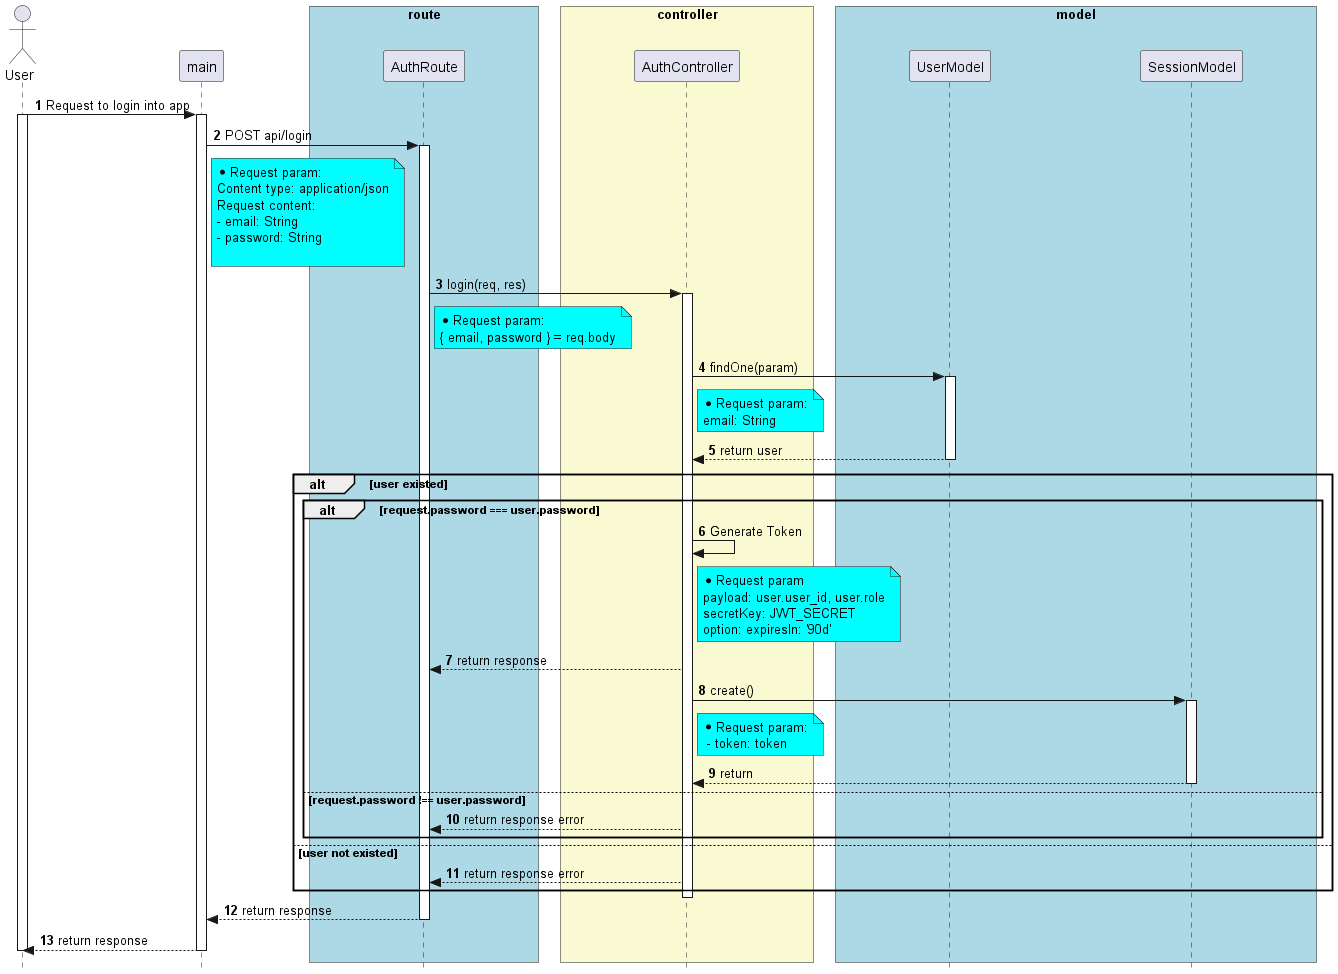
\includegraphics[width=16cm,height=12cm]{Images/server/sequence/server/login.png}
  \caption[Sơ đồ tuần tự cho API đăng nhập vào hệ thống]{\bfseries \fontsize{12pt}{0pt}
  \selectfont Sơ đồ tuần tự cho API đăng nhập vào hệ thống }
  \label{backend_login} %đặt tên cho ảnh
\end{figure}
Hình \ref{backend_login}  mô tả quá trình xác thực người dùng đăng nhập vào ứng dụng. Người dùng gửi yêu cầu đăng nhập, thông qua các tầng của hệ thống, yêu cầu này được xử lý bởi AuthController. AuthController kiểm tra thông tin người dùng, tạo token nếu đúng thông tin đăng nhập và trả về response cho người dùng.

\begin{figure}[H]
  \centering
  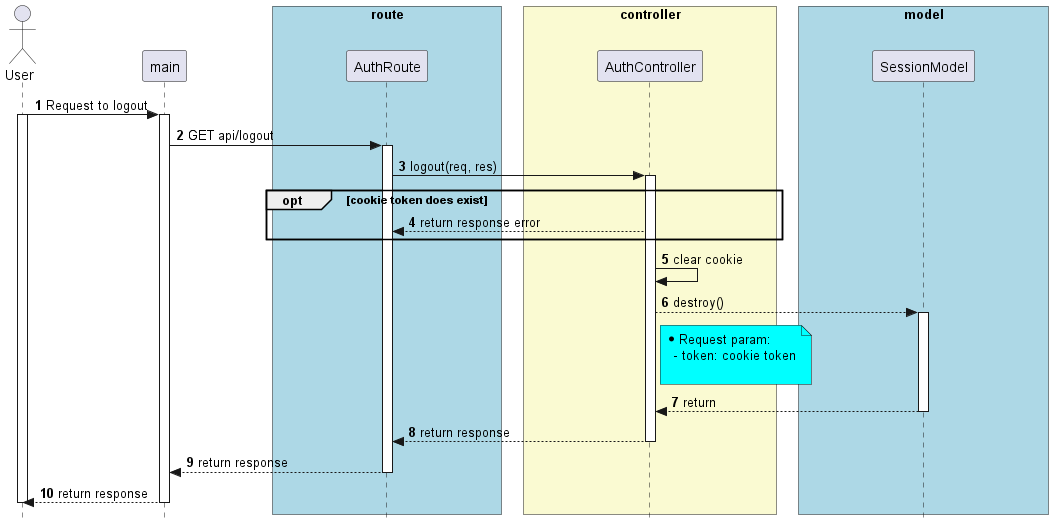
\includegraphics[width=16cm,height=9cm]{Images/server/sequence/server/logout.png}
  \caption[Sơ đồ tuần tự cho API đăng xuất khỏi hệ thống ]{\bfseries \fontsize{12pt}{0pt}
  \selectfont Sơ đồ tuần tự cho API đăng xuất khỏi hệ thống }
  \label{backend_logout} %đặt tên cho ảnh
\end{figure}
Hình \ref{backend_logout} mô tả quá trình đăng xuất (logout) người dùng khỏi ứng dụng. Người dùng gửi yêu cầu đăng xuất, thông qua các tầng của hệ thống, yêu cầu này được xử lý bởi AuthController. Đầu tiên, hệ thống kiểm tra xem cookie token có tồn tại hay không. Nếu không tồn tại, hệ thống trả về response lỗi. Ngược lại, AuthController xóa cookie và gọi tới SessionModel để hủy phiên đăng nhập của người dùng dựa trên token trong cookie. Sau khi xử lý, hệ thống trả về response thành công tới người dùng.

\begin{figure}[H]
  \centering
  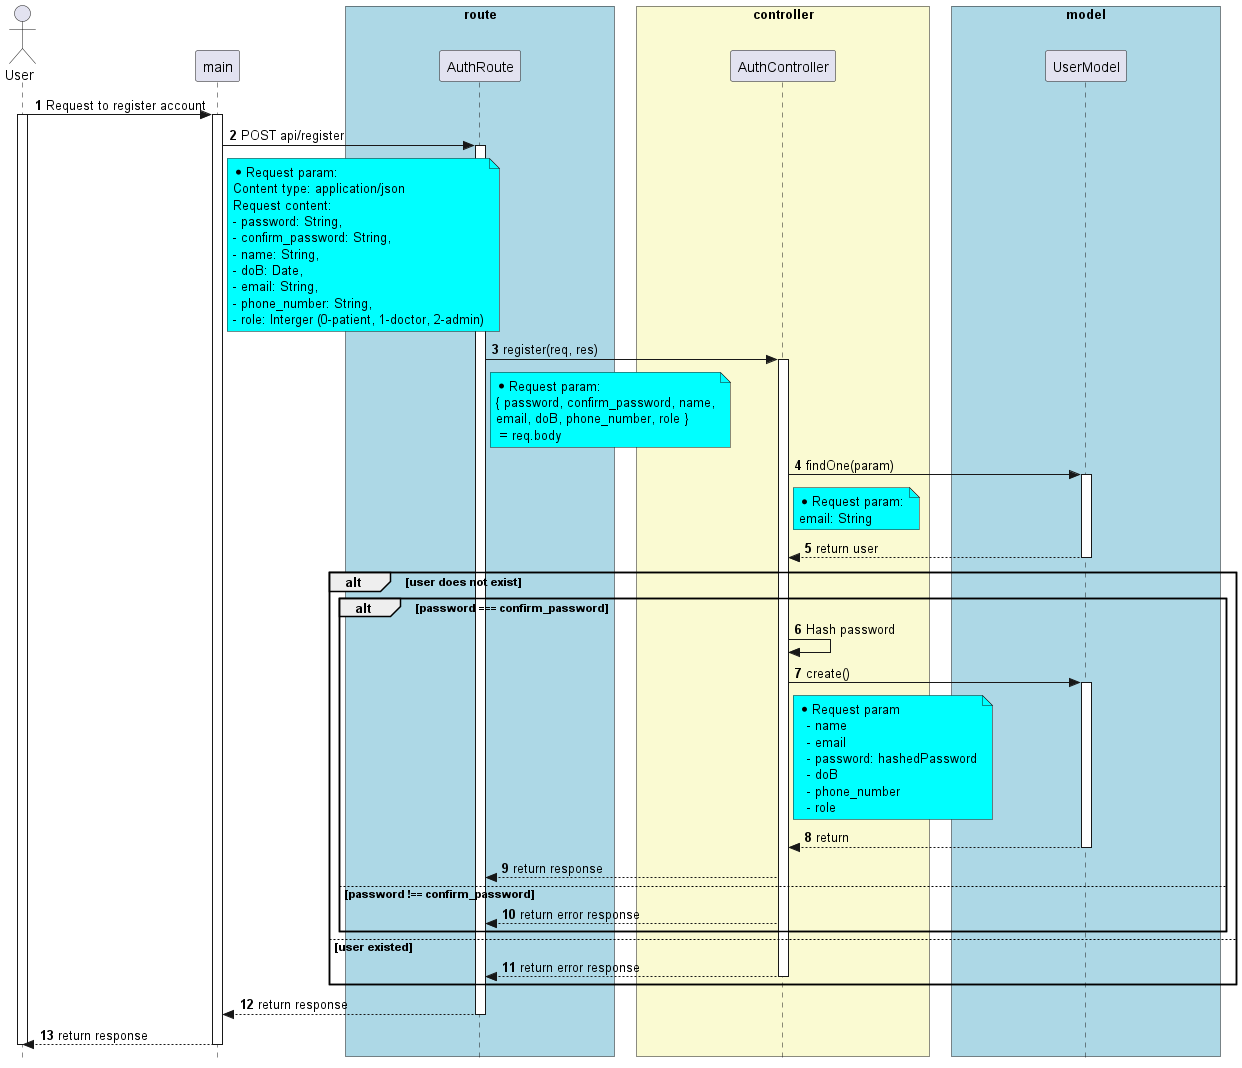
\includegraphics[width=16cm,height=12cm]{Images/server/sequence/server/register.png}
  \caption[Sơ đồ tuần tự cho API đăng ký tài khoản]{\bfseries \fontsize{12pt}{0pt}
  \selectfont Sơ đồ tuần tự cho API đăng ký tài khoản }
  \label{backend_register} %đặt tên cho ảnh
\end{figure}
Hình \ref{backend_register} mô tả quá trình đăng ký tài khoản trong ứng dụng. Người dùng gửi yêu cầu đăng ký, thông qua các tầng của hệ thống, yêu cầu này được xử lý bởi AuthController. Đầu tiên, hệ thống kiểm tra thông tin yêu cầu đăng ký, bao gồm việc kiểm tra mật khẩu và xác nhận mật khẩu có khớp hay không. Sau đó, AuthController kiểm tra xem người dùng đã tồn tại trong hệ thống hay chưa. Nếu người dùng chưa tồn tại và mật khẩu khớp, AuthController sẽ mã hóa mật khẩu và tạo một bản ghi mới trong UserModel để lưu thông tin đăng ký. Nếu người dùng đã tồn tại hoặc mật khẩu không khớp, hệ thống sẽ trả về response lỗi tương ứng. Sau khi xử lý, hệ thống trả về response kết quả cho người dùng.


\begin{figure}[H]
  \centering
  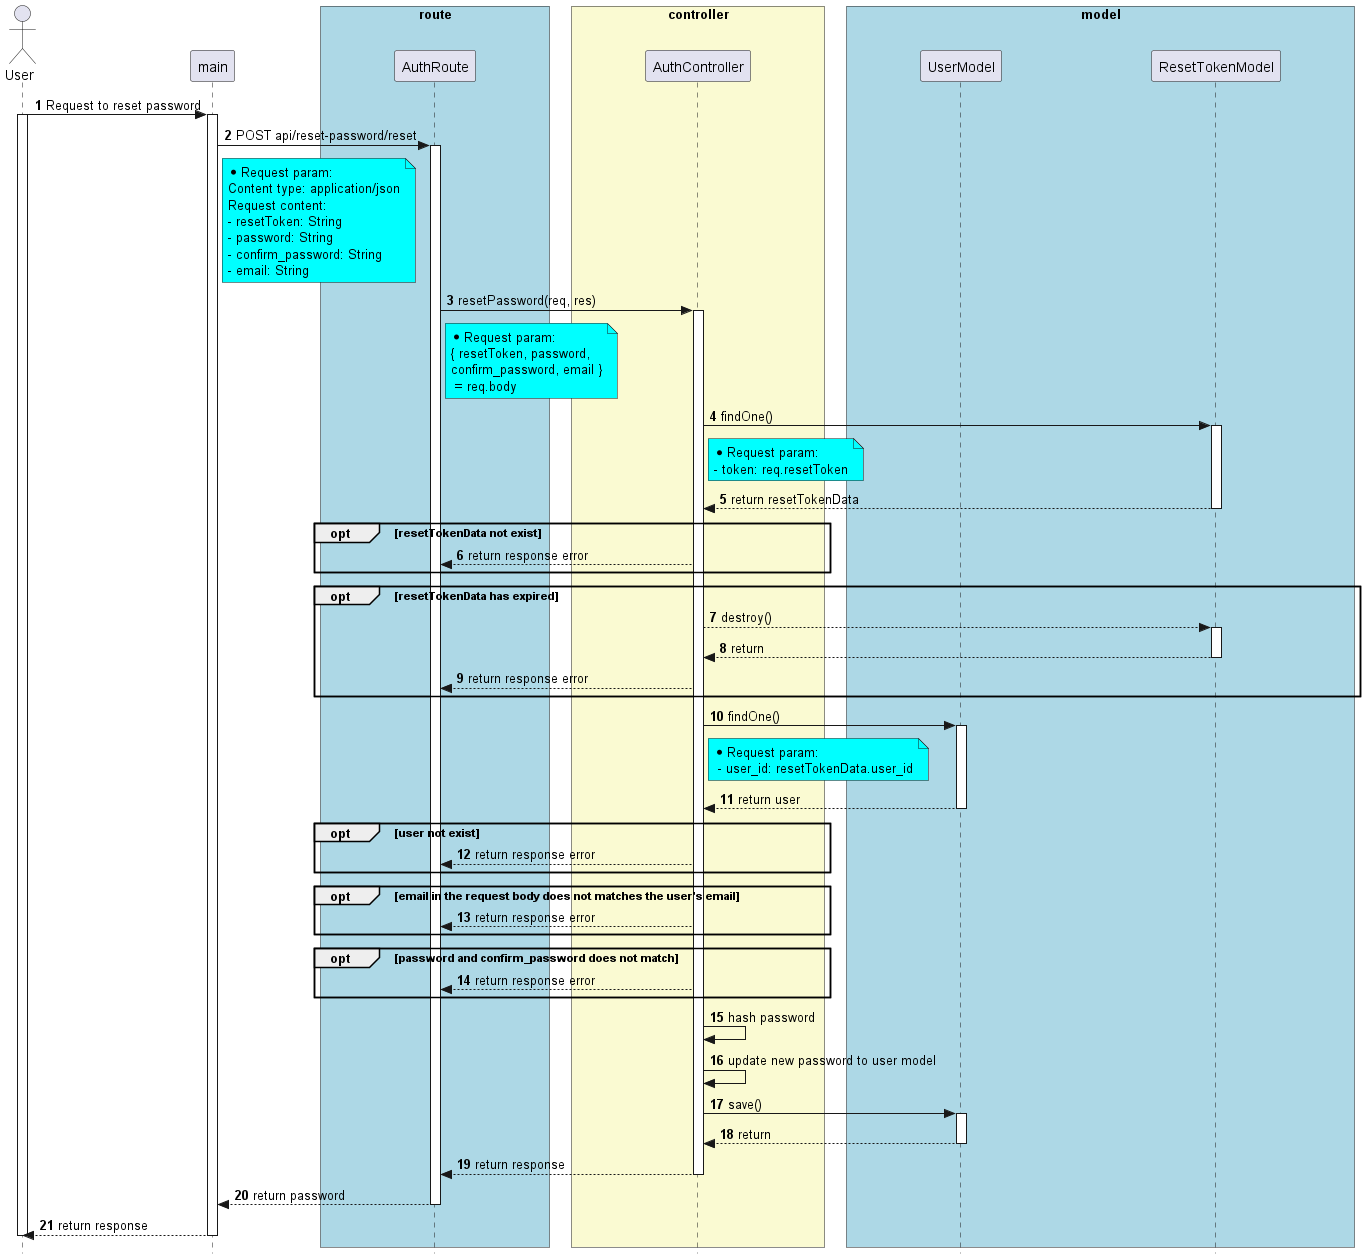
\includegraphics[width=16cm,height=13cm]{Images/server/sequence/server/resetPassword.png}
  \caption[Sơ đồ tuần tự cho API đăt lại mật khẩu ]{\bfseries \fontsize{12pt}{0pt}
  \selectfont Sơ đồ tuần tự cho API đăt lại mật khẩu }
  \label{resetPassword} %đặt tên cho ảnh
\end{figure}
Hình \ref{resetPassword} mô tả quá trình đặt lại mật khẩu (reset password) trong ứng dụng. Người dùng gửi yêu cầu đặt lại mật khẩu, thông qua các tầng của hệ thống, yêu cầu này được xử lý bởi AuthController. Đầu tiên, hệ thống kiểm tra thông tin yêu cầu đặt lại mật khẩu, bao gồm resetToken, mật khẩu mới và xác nhận mật khẩu. Sau đó, AuthController kiểm tra xem resetToken có hợp lệ hay không, bằng cách tìm kiếm trong ResetTokenModel. Nếu resetToken không hợp lệ hoặc đã hết hạn, hệ thống sẽ trả về response lỗi tương ứng. Nếu resetToken hợp lệ, AuthController tiếp tục kiểm tra xem người dùng có tồn tại và email trong yêu cầu có khớp với email của người dùng không. Nếu không hợp lệ, hệ thống sẽ trả về response lỗi tương ứng. Nếu mọi thông tin đều hợp lệ, AuthController sẽ mã hóa mật khẩu mới, cập nhật mật khẩu trong UserModel và trả về response thành công tới người dùng.

\begin{figure}[H]
  \centering
  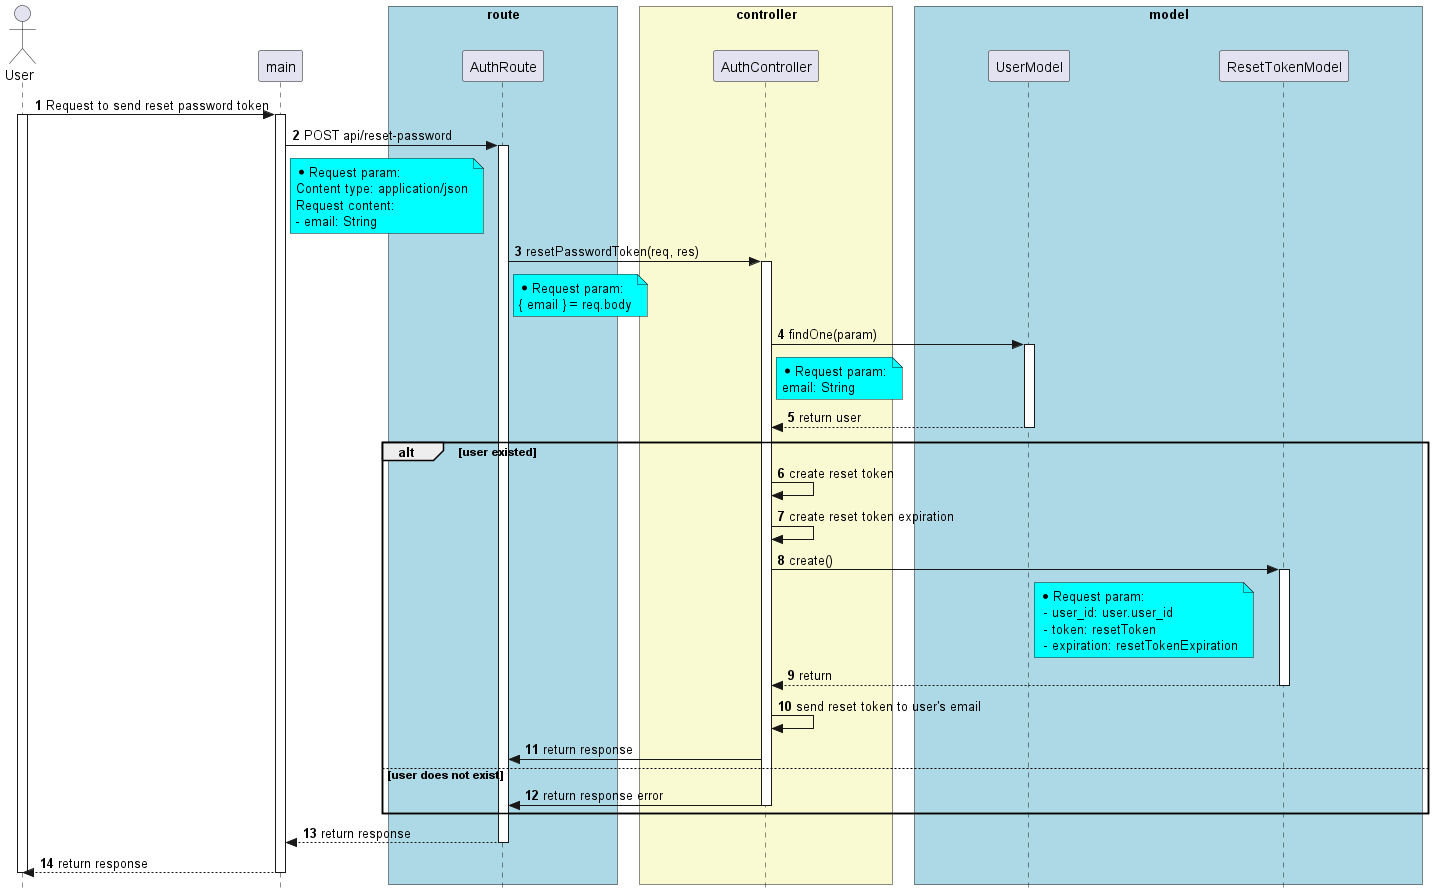
\includegraphics[width=16cm,height=9cm]{Images/server/sequence/server/resetPasswordToken.png}
  \caption[Sơ đồ tuần tự cho API gửi token đặt lại mật khẩu ]{\bfseries \fontsize{12pt}{0pt}
  \selectfont Sơ đồ tuần tự cho API gửi token đặt lại mật khẩu  }
  \label{resetPasswordToken} %đặt tên cho ảnh
\end{figure}
Hình \ref{resetPasswordToken} mô tả quá trình yêu cầu gửi mã thông báo đặt lại mật khẩu (reset password token) trong ứng dụng. Người dùng gửi yêu cầu đặt lại mật khẩu, thông qua các tầng của hệ thống, yêu cầu này được xử lý bởi AuthController. Đầu tiên, hệ thống kiểm tra thông tin yêu cầu đặt lại mật khẩu, bao gồm email người dùng. Sau đó, AuthController kiểm tra xem người dùng đã tồn tại trong hệ thống hay chưa. Nếu người dùng tồn tại, AuthController sẽ tạo một mã thông báo đặt lại mật khẩu (reset token) cùng với thời gian hết hạn cho mã (reset token expiration) và lưu thông tin này vào ResetTokenModel. Sau đó, hệ thống sẽ gửi mã thông báo đặt lại mật khẩu tới email của người dùng. Nếu người dùng không tồn tại, hệ thống sẽ trả về response lỗi tương ứng. Sau khi xử lý, hệ thống trả về response kết quả cho người dùng.

% ----------------------------------------------


% ------------------------News----------------------
\paragraph{API liên quan đến tin tức}
\mbox{}


\begin{figure}[H]
  \centering
  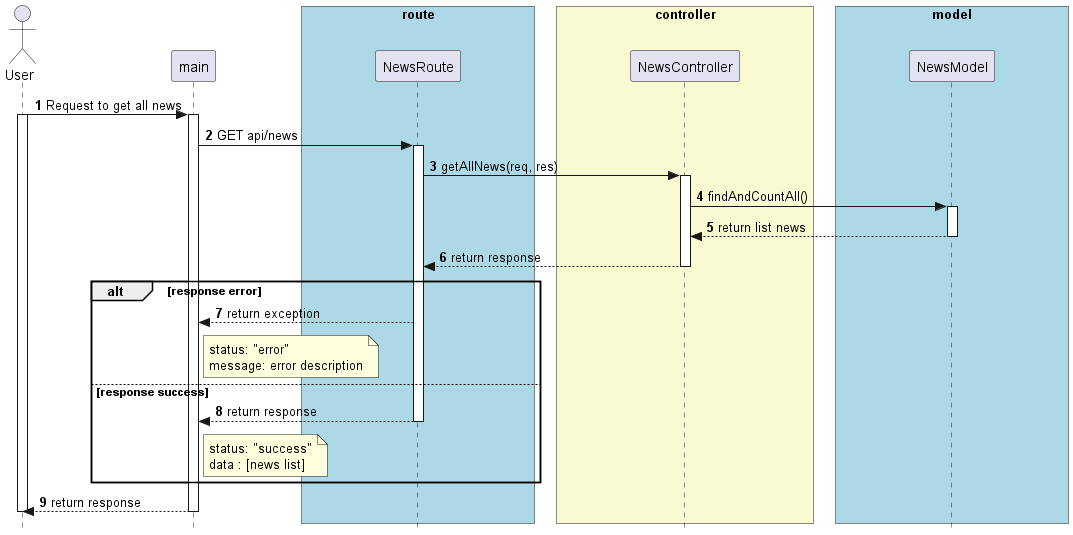
\includegraphics[width=16cm,height=9cm]{Images/server/sequence/server/getAllNews.png}
  \caption[Sơ đồ tuần tự cho API lấy tất cả thông tin của tin tức]{\bfseries \fontsize{12pt}{0pt}
  \selectfont Sơ đồ tuần tự cho API lấy tất cả thông tin của tin tức }
  \label{getAllNews} %đặt tên cho ảnh
\end{figure}
Hình \ref{getAllNews} mô tả quá trình lấy tất cả tin tức (news) trong ứng dụng. Người dùng gửi yêu cầu lấy tất cả tin tức, thông qua các tầng của hệ thống, yêu cầu này được xử lý bởi NewsController. NewsController tiếp tục truy vấn NewsModel để lấy danh sách tất cả các tin tức từ cơ sở dữ liệu. Sau đó, danh sách tin tức được trả về từ NewsModel và được gửi trở lại NewsRoute để trả về response cho người dùng. Nếu quá trình thực hiện thành công, hệ thống trả về response chứa danh sách tin tức cho người dùng. Nếu có lỗi xảy ra trong quá trình này, hệ thống trả về response lỗi với mô tả lỗi tương ứng. Sau khi xử lý, response cuối cùng được trả về tới người dùng.


\begin{figure}[H]
  \centering
  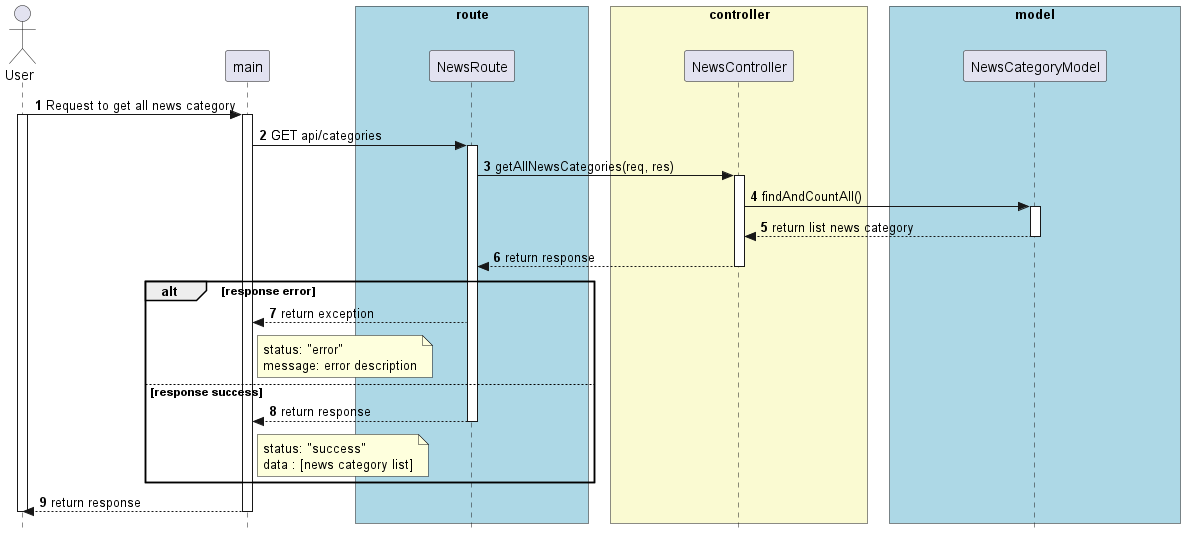
\includegraphics[width=16cm,height=9cm]{Images/server/sequence/server/getAllNewsCategories.png}
  \caption[Sơ đồ tuần tự cho API lấy tất cả thông tin của danh mục tin tức ]{\bfseries \fontsize{12pt}{0pt}
  \selectfont Sơ đồ tuần tự cho API lấy tất cả thông tin của danh mục tin tức }
  \label{getAllNewsCategories} %đặt tên cho ảnh
\end{figure}
Hình \ref{getAllNewsCategories} mô tả quá trình lấy tất cả danh mục tin tức (news category) trong ứng dụng. Người dùng gửi yêu cầu lấy tất cả danh mục tin tức, thông qua các tầng của hệ thống, yêu cầu này được xử lý bởi NewsController. NewsController tiếp tục truy vấn NewsCategoryModel để lấy danh sách tất cả các danh mục tin tức từ cơ sở dữ liệu. Sau đó, danh sách danh mục tin tức được trả về từ NewsCategoryModel và được gửi trở lại NewsRoute để trả về response cho người dùng. Nếu quá trình thực hiện thành công, hệ thống trả về response chứa danh sách danh mục tin tức cho người dùng. Nếu có lỗi xảy ra trong quá trình này, hệ thống trả về response lỗi với mô tả lỗi tương ứng. Sau khi xử lý, response cuối cùng được trả về tới người dùng.

\begin{figure}[H]
  \centering
  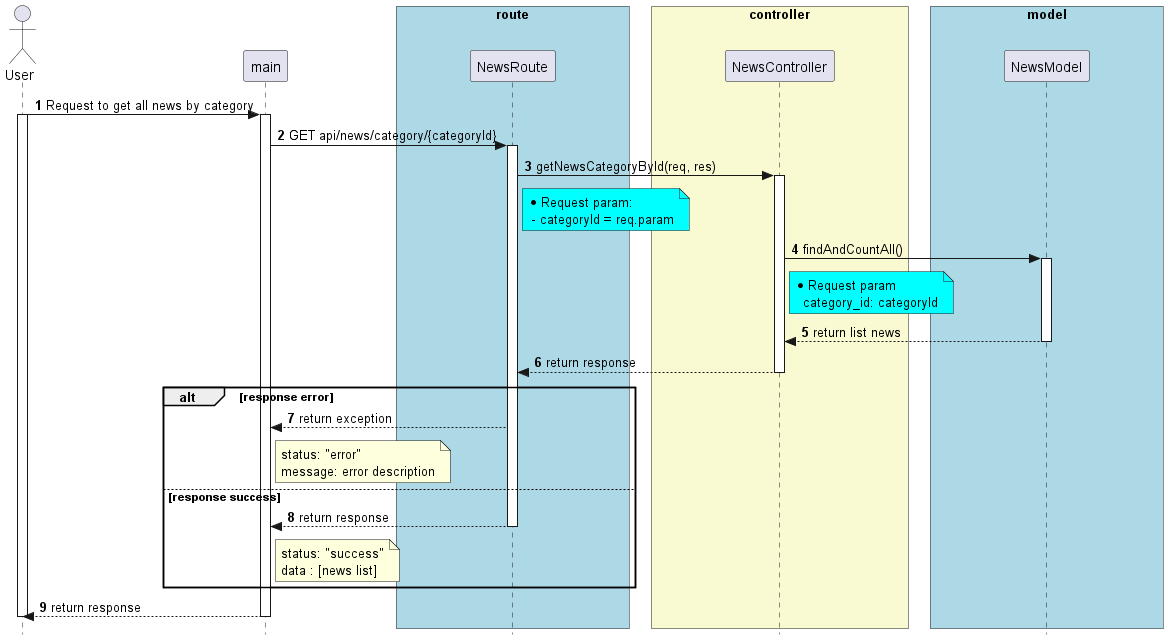
\includegraphics[width=16cm,height=9cm]{Images/server/sequence/server/getNewsByCategory.png}
  \caption[Sơ đồ tuần tự cho API lấy tất cả tin tức theo loại tin tức ]{\bfseries \fontsize{12pt}{0pt}
  \selectfont Sơ đồ tuần tự cho API lấy tất cả tin tức theo danh mục tin tức }
  \label{getNewsByCategory} %đặt tên cho ảnh
\end{figure}
Hình \ref{getNewsByCategory} mô tả quá trình lấy danh sách tin tức (news list) theo danh mục (category) trong ứng dụng. Người dùng gửi yêu cầu lấy danh sách tin tức theo danh mục, thông qua các tầng của hệ thống, yêu cầu này được xử lý bởi NewsController. NewsController tiếp tục truy vấn NewsModel để lấy danh sách tin tức dựa trên categoryId được truyền vào từ yêu cầu. Sau đó, danh sách tin tức được trả về từ NewsModel và được gửi trở lại NewsRoute để trả về response cho người dùng. Nếu quá trình thực hiện thành công, hệ thống trả về response chứa danh sách tin tức cho người dùng. Nếu có lỗi xảy ra trong quá trình này, hệ thống trả về response lỗi tương ứng. Sau khi xử lý, response cuối cùng được trả về tới người dùng.


\begin{figure}[H]
  \centering
  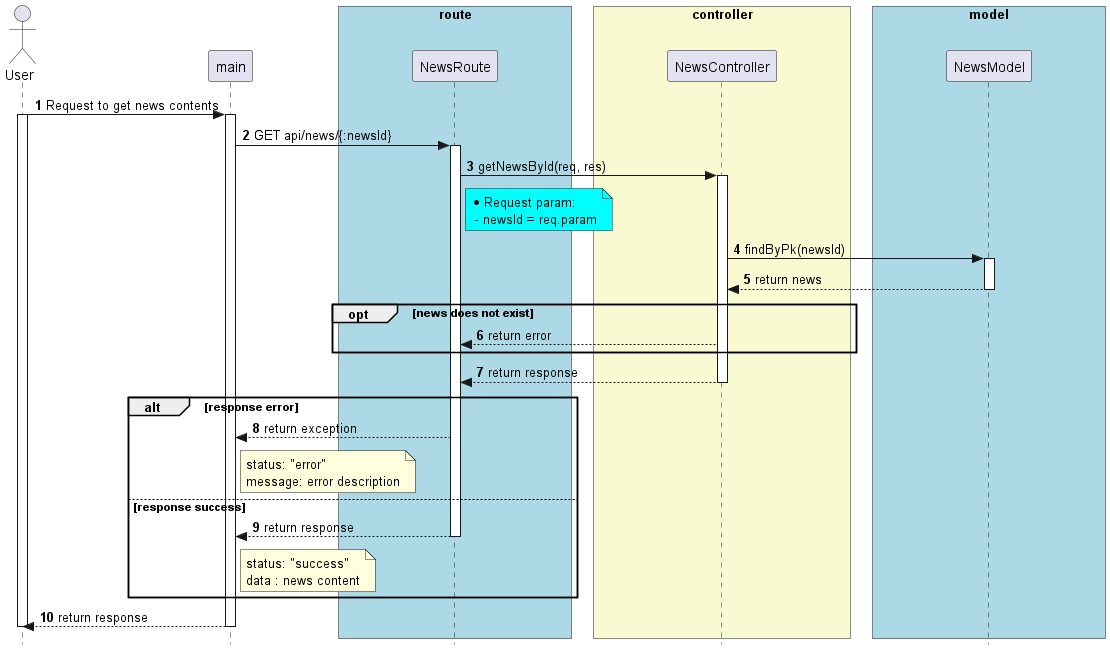
\includegraphics[width=16cm,height=9cm]{Images/server/sequence/server/getNewsById.png}
  \caption[Sơ đồ tuần tự cho API lấy nội dung của một tin tức ]{\bfseries \fontsize{12pt}{0pt}
  \selectfont Sơ đồ tuần tự cho API lấy nội dung của một tin tức }
  \label{getNewsById} %đặt tên cho ảnh
\end{figure}
Hình \ref{getNewsById} mô tả quá trình lấy nội dung tin tức (news content) trong ứng dụng. Người dùng gửi yêu cầu lấy nội dung tin tức, thông qua các tầng của hệ thống, yêu cầu này được xử lý bởi NewsController. NewsController tiếp tục truy vấn NewsModel để lấy nội dung tin tức dựa trên newsId được truyền vào từ yêu cầu. Sau đó, nội dung tin tức được trả về từ NewsModel và được gửi trở lại NewsRoute để trả về response cho người dùng. Nếu quá trình thực hiện thành công, hệ thống trả về response chứa nội dung tin tức cho người dùng. Nếu tin tức không tồn tại, hệ thống trả về response lỗi tương ứng. Nếu có lỗi xảy ra trong quá trình này, hệ thống trả về response lỗi với mô tả lỗi tương ứng. Sau khi xử lý, response cuối cùng được trả về tới người dùng.

\begin{figure}[H]
  \centering
  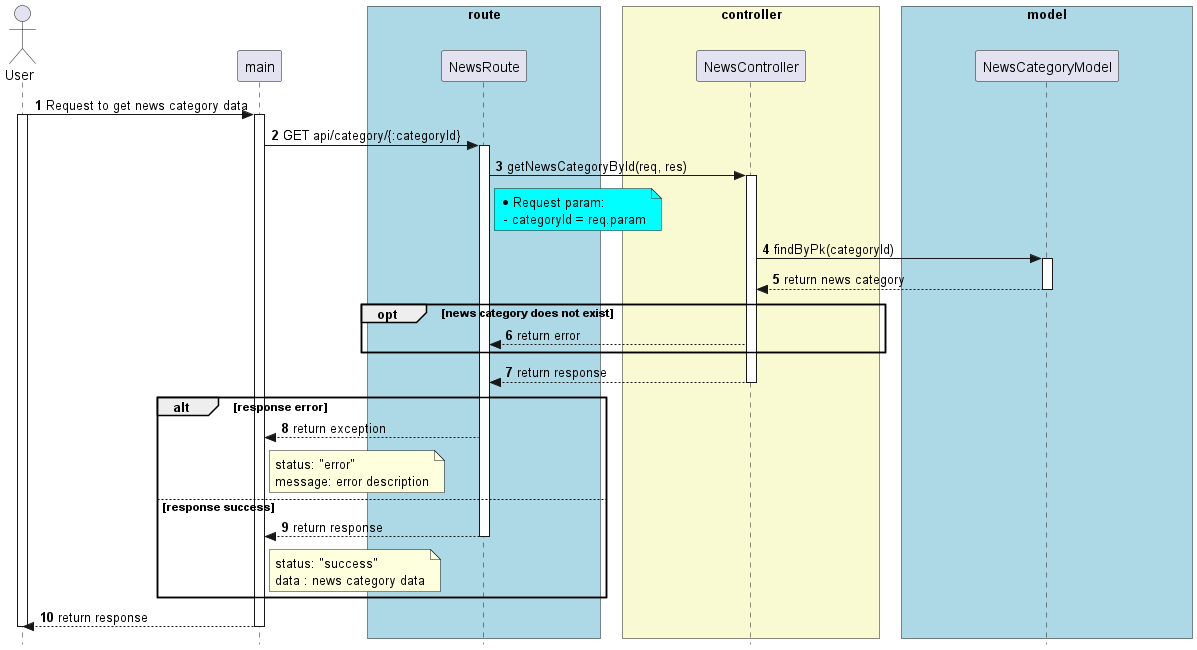
\includegraphics[width=16cm,height=9cm]{Images/server/sequence/server/getNewsCategoryById.png}
  \caption[Sơ đồ tuần tự cho API lấy thông tin của một danh mục tin tức ]{\bfseries \fontsize{12pt}{0pt}
  \selectfont Sơ đồ tuần tự cho API lấy thông tin của một danh mục tin tức }
  \label{getNewsCategoryById} %đặt tên cho ảnh
\end{figure}
Hình \ref{getNewsCategoryById} mô tả quá trình lấy dữ liệu danh mục tin tức (news category data) trong ứng dụng. Người dùng gửi yêu cầu lấy dữ liệu danh mục tin tức, thông qua các tầng của hệ thống, yêu cầu này được xử lý bởi NewsController. NewsController tiếp tục truy vấn NewsCategoryModel để lấy dữ liệu danh mục tin tức dựa trên categoryId được truyền vào từ yêu cầu. Sau đó, dữ liệu danh mục tin tức được trả về từ NewsCategoryModel và được gửi trở lại NewsRoute để trả về response cho người dùng. Nếu quá trình thực hiện thành công, hệ thống trả về response chứa dữ liệu danh mục tin tức cho người dùng. Nếu danh mục tin tức không tồn tại, hệ thống trả về response lỗi tương ứng. Nếu có lỗi xảy ra trong quá trình này, hệ thống trả về response lỗi với mô tả lỗi tương ứng. Sau khi xử lý, response cuối cùng được trả về tới người dùng.

% -----------------------------------------------------


% -------------------------ECG----------------------------
\paragraph{API liên quan đến bản ghi ECG}
\mbox{}



\begin{figure}[H]
  \centering
  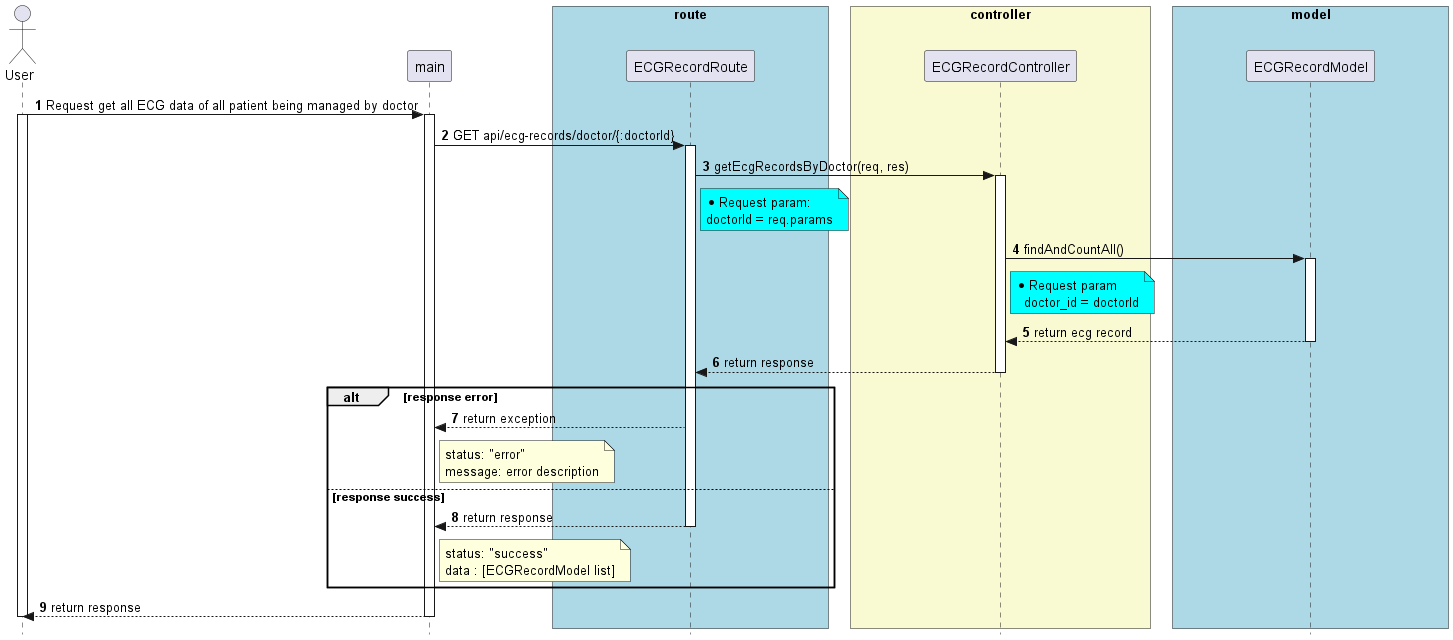
\includegraphics[width=16cm,height=9cm]{Images/server/sequence/server/getEcgRecordsByDoctor.png}
  \caption[Sơ đồ tuần tự cho API lấy thông tin phiên đo ECG của các bệnh nhân được quản lý bởi một bác sĩ ]{\bfseries \fontsize{12pt}{0pt}
  \selectfont Sơ đồ tuần tự cho API lấy thông tin phiên đo ECG của các bệnh nhân được quản lý bởi một bác sĩ }
  \label{getEcgRecordsByDoctor} %đặt tên cho ảnh
\end{figure}
Hình \ref{getEcgRecordsByDoctor} mô tả quá trình lấy dữ liệu ECG (Electrocardiogram) của tất cả bệnh nhân được quản lý bởi một bác sĩ trong ứng dụng. Người dùng (bác sĩ) gửi yêu cầu lấy dữ liệu ECG của tất cả bệnh nhân mà họ quản lý, thông qua các tầng của hệ thống, yêu cầu này được xử lý bởi ECGRecordController. ECGRecordController tiếp tục truy vấn ECGRecordModel để lấy dữ liệu ECG dựa trên doctorId (ID của bác sĩ) được truyền vào từ yêu cầu. Sau đó, danh sách dữ liệu ECG của các bệnh nhân được trả về từ ECGRecordModel và được gửi trở lại ECGRecordRoute để trả về response cho người dùng. Nếu quá trình thực hiện thành công, hệ thống trả về response chứa danh sách dữ liệu ECG cho bác sĩ. Nếu có lỗi xảy ra trong quá trình này, hệ thống trả về response lỗi tương ứng. Sau khi xử lý, response cuối cùng được trả về tới người dùng (bác sĩ).


\begin{figure}[H]
  \centering
  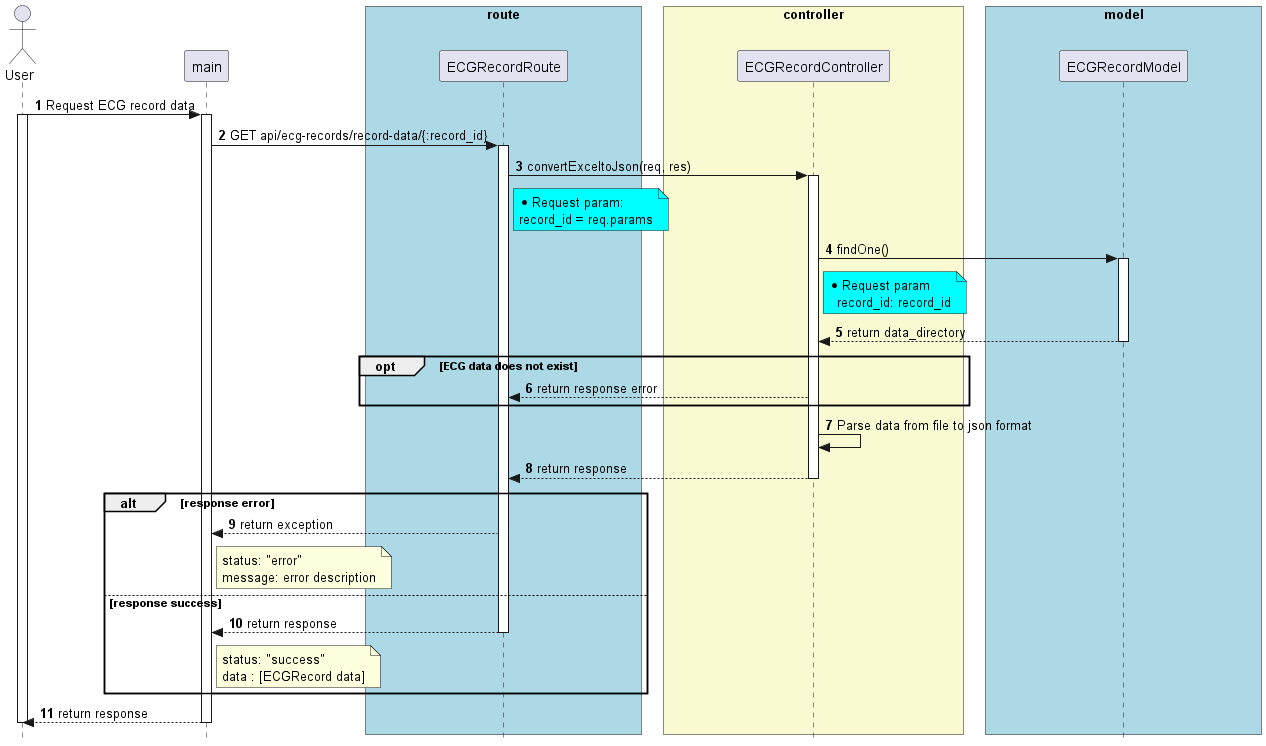
\includegraphics[width=16cm,height=9cm]{Images/server/sequence/server/convertExceltoJson.png}
  \caption[Sơ đồ tuần tự cho API lấy dữ liệu của một phiên đo ECG ]{\bfseries \fontsize{12pt}{0pt}
  \selectfont Sơ đồ tuần tự cho API lấy dữ liệu của một phiên đo ECG  }
  \label{convertExceltoJson} %đặt tên cho ảnh
\end{figure}
Hình \ref{convertExceltoJson} mô tả quá trình yêu cầu lấy dữ liệu ECG (Electrocardiogram) từ một bản ghi cụ thể trong ứng dụng. Người dùng (User) gửi yêu cầu lấy dữ liệu ECG cho một bản ghi có record\_id nhất định, thông qua các tầng của hệ thống, yêu cầu này được xử lý bởi ECGRecordController. ECGRecordController tiếp tục truy vấn ECGRecordModel để tìm kiếm bản ghi ECG dựa trên record\_id được truyền vào từ yêu cầu. Sau đó, data\_directory của bản ghi ECG được trả về từ ECGRecordModel và được gửi trở lại ECGRecordRoute để xử lý việc chuyển đổi dữ liệu từ định dạng file Excel sang định dạng JSON. Nếu quá trình thực hiện thành công, hệ thống trả về response chứa dữ liệu ECG của bản ghi tương ứng. Nếu có lỗi xảy ra trong quá trình này, hệ thống trả về response lỗi tương ứng. Sau khi xử lý, response cuối cùng được trả về tới người dùng.

\begin{figure}[H]
  \centering
  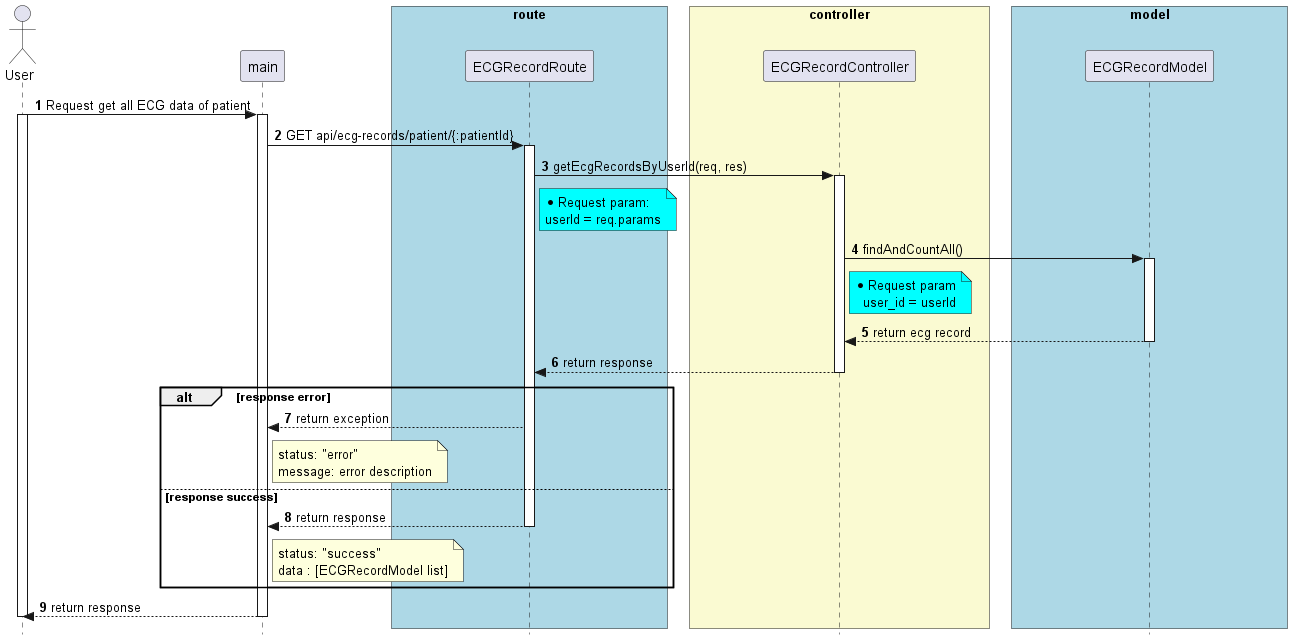
\includegraphics[width=16cm,height=9cm]{Images/server/sequence/server/getEcgRecordsByUserId.png}
  \caption[Sơ đồ tuần tự cho API lấy thông tin các phiên đo ECG của một bệnh nhân]{\bfseries \fontsize{12pt}{0pt}
  \selectfont Sơ đồ tuần tự cho API lấy thông tin các phiên đo ECG của một bệnh nhân }
  \label{getEcgRecordsByUserId} %đặt tên cho ảnh
\end{figure}
Hình \ref{getEcgRecordsByUserId} mô tả quá trình yêu cầu dữ liệu ECG (Electrocardiogram) của một bệnh nhân cụ thể từ ứng dụng. Người dùng (User) gửi yêu cầu lấy dữ liệu ECG cho một bệnh nhân với patientId nhất định, thông qua các tầng của hệ thống, yêu cầu này được xử lý bởi ECGRecordController. ECGRecordController tiếp tục truy vấn ECGRecordModel để tìm kiếm các bản ghi ECG của bệnh nhân dựa trên patientId được truyền vào từ yêu cầu. Sau đó, danh sách các bản ghi ECG của bệnh nhân được trả về từ ECGRecordModel và được gửi trở lại ECGRecordRoute để tạo response chứa danh sách này. Nếu quá trình thực hiện thành công, hệ thống trả về response chứa danh sách các bản ghi ECG của bệnh nhân tương ứng. Nếu có lỗi xảy ra trong quá trình này, hệ thống trả về response lỗi tương ứng. Sau khi xử lý, response cuối cùng được trả về tới người dùng.


\begin{figure}[H]
  \centering
  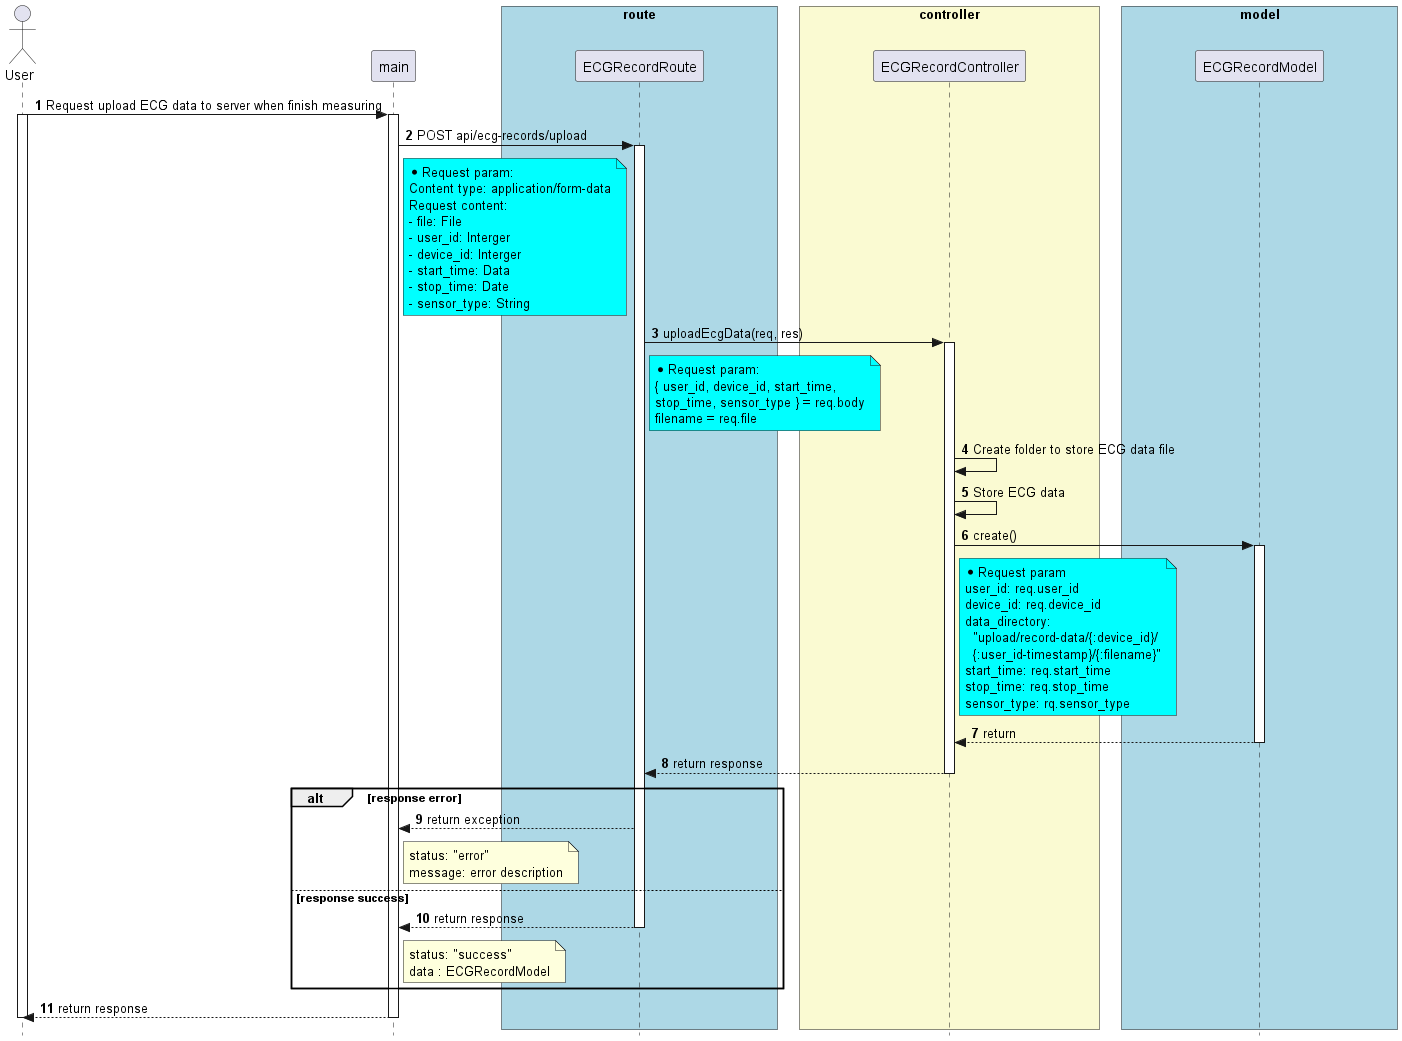
\includegraphics[width=16cm,height=13cm]{Images/server/sequence/server/uploadEcgData.png}
  \caption[Sơ đồ tuần tự cho API tải dữ liệu ECG lên server ]{\bfseries \fontsize{12pt}{0pt}
  \selectfont Sơ đồ tuần tự cho API tải dữ liệu ECG lên server }
  \label{uploadEcgData} %đặt tên cho ảnh
\end{figure}
Hình \ref{uploadEcgData} mô tả quá trình tải lên dữ liệu ECG (Electrocardiogram) sau khi hoàn thành việc đo đạc từ thiết bị đo ECG. Người dùng (User) gửi yêu cầu tải lên dữ liệu ECG cho một bệnh nhân cụ thể, thông qua các tầng của hệ thống, yêu cầu này được xử lý bởi ECGRecordController. ECGRecordController tiếp tục tạo folder mới để lưu trữ dữ liệu ECG, sau đó lưu dữ liệu ECG được tải lên vào folder vừa tạo. Tiếp theo, ECGRecordController tạo một bản ghi mới trong ECGRecordModel, lưu trữ thông tin về người dùng (user\_id), thiết bị đo (device\_id), thời gian bắt đầu đo (start\_time), thời gian kết thúc đo (stop\_time), loại cảm biến (sensor\_type) và đường dẫn của dữ liệu ECG được lưu trữ. Sau đó, ECGRecordModel trả về thông tin vừa lưu vào ECGRecordController. Nếu quá trình tải lên thành công, hệ thống trả về response thành công chứa thông tin về bản ghi ECG vừa tạo. Nếu có lỗi xảy ra trong quá trình này, hệ thống trả về response lỗi tương ứng. Sau khi xử lý, response cuối cùng được trả về tới người dùng.
% -----------------------------------------------------



% -----------------------PatientDoctor------------------------------
\paragraph{API liên quan liên quan đến việc phân công bệnh nhân cho bác sỹ}
\mbox{}


\begin{figure}[H]
  \centering
  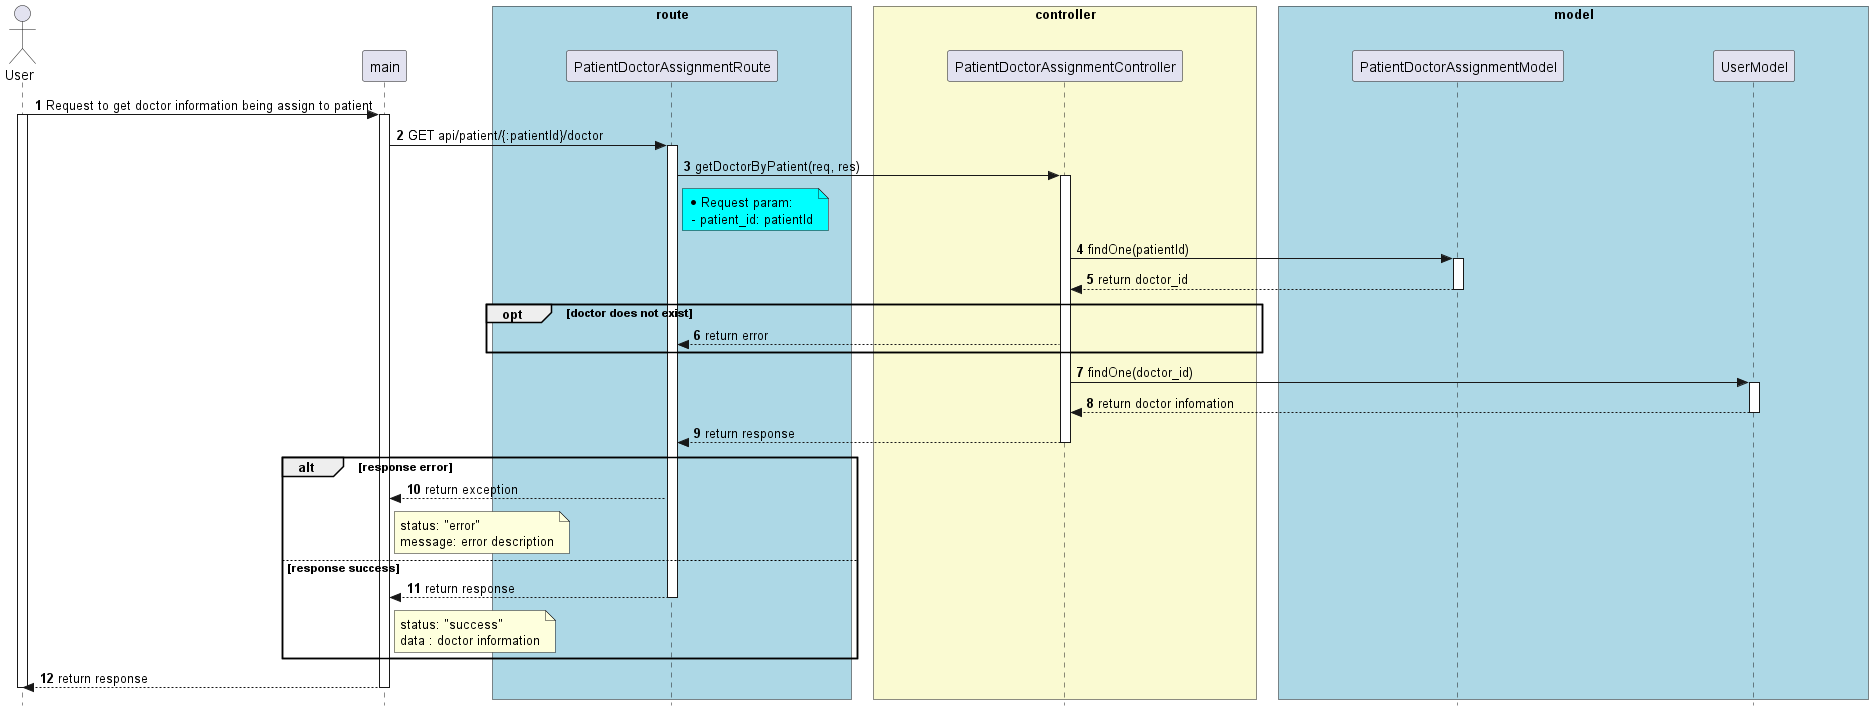
\includegraphics[width=16cm,height=10cm]{Images/server/sequence/server/getDoctorByPatient.png}
  \caption[Sơ đồ tuần tự cho API lấy thông tin bác sĩ được phân công cho một bệnh nhân ]{\bfseries \fontsize{12pt}{0pt}
  \selectfont Sơ đồ tuần tự cho API lấy thông tin bác sĩ được phân công cho một bệnh nhân }
  \label{getDoctorByPatient} %đặt tên cho ảnh
\end{figure}
Hình \ref{getDoctorByPatient} mô tả quá trình lấy thông tin bác sĩ được phân công cho một bệnh nhân cụ thể. Người dùng (User) gửi yêu cầu lấy thông tin bác sĩ của một bệnh nhân cụ thể, thông qua các tầng của hệ thống, yêu cầu này được xử lý bởi PatientDoctorAssignmentController. PatientDoctorAssignmentController tìm kiếm thông tin liên kết giữa bệnh nhân và bác sĩ trong PatientDoctorAssignmentModel bằng cách tìm bản ghi với patient\_id trùng khớp với bệnh nhân được chỉ định. Nếu không tìm thấy thông tin liên kết, hệ thống trả về response lỗi tương ứng. Nếu tìm thấy thông tin liên kết, PatientDoctorAssignmentController sẽ tiếp tục tìm kiếm thông tin của bác sĩ trong UserModel bằng cách sử dụng doctor\_id lấy từ bản ghi liên kết. Sau khi tìm thấy thông tin của bác sĩ, hệ thống trả về response thành công chứa thông tin về bác sĩ đó. Nếu có lỗi xảy ra trong quá trình này, hệ thống trả về response lỗi tương ứng. Sau khi xử lý, response cuối cùng được trả về tới người dùng.


\begin{figure}[H]
  \centering
  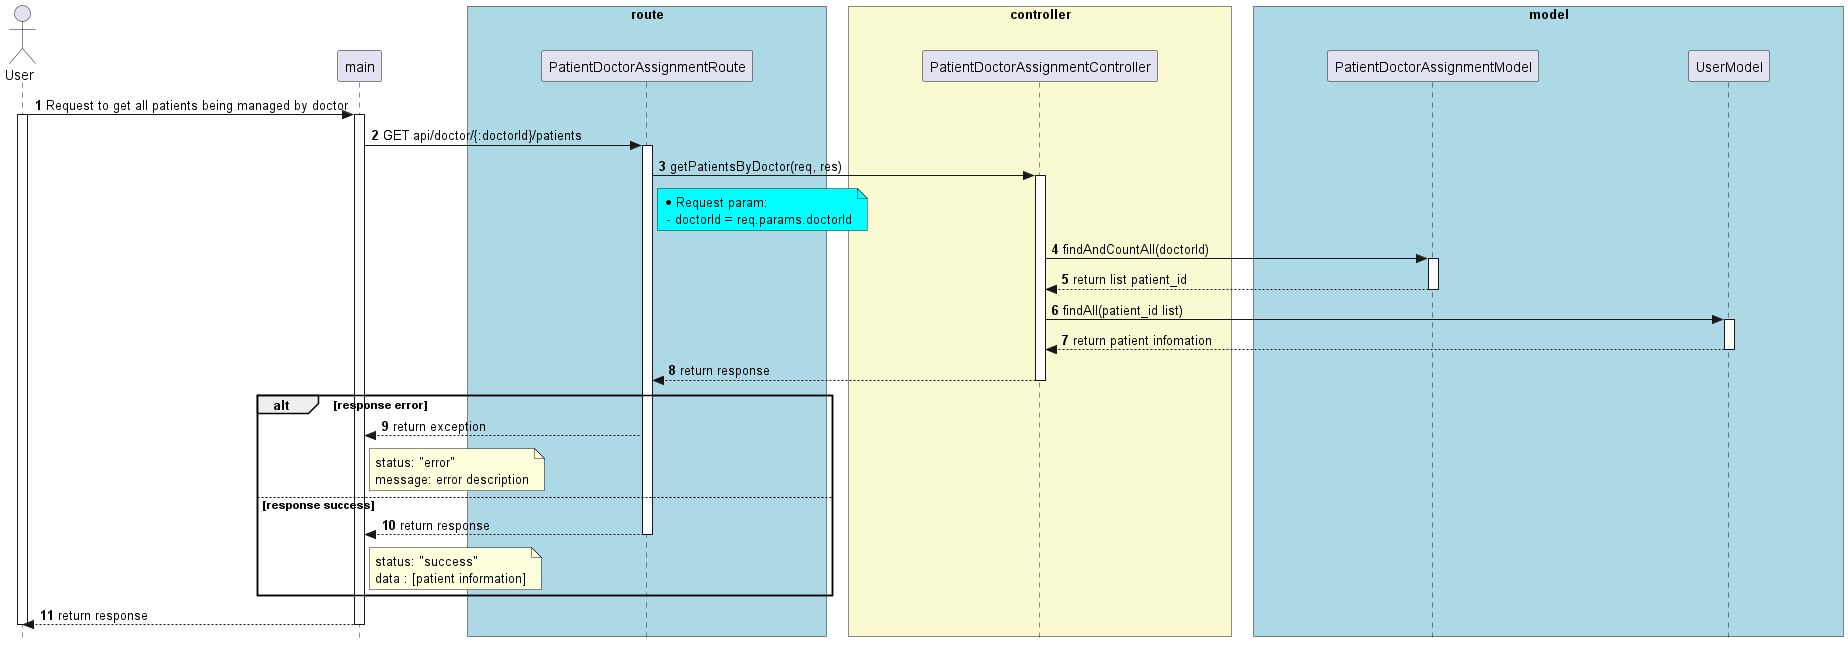
\includegraphics[width=16cm,height=9cm]{Images/server/sequence/server/getPatientsByDoctor.png}
  \caption[Sơ đồ tuần tự cho API lấy thông tin tất cả bệnh nhân được quản lý bởi một bác sĩ]{\bfseries \fontsize{12pt}{0pt}
  \selectfont Sơ đồ tuần tự cho API lấy thông tin tất cả bệnh nhân được quản lý bởi một bác sĩ }
  \label{getPatientsByDoctor} %đặt tên cho ảnh
\end{figure}
Hình \ref{getPatientsByDoctor}  mô tả quá trình lấy thông tin tất cả bệnh nhân được quản lý bởi một bác sĩ cụ thể. Người dùng (User) gửi yêu cầu lấy thông tin tất cả bệnh nhân của một bác sĩ cụ thể, thông qua các tầng của hệ thống, yêu cầu này được xử lý bởi PatientDoctorAssignmentController. PatientDoctorAssignmentController tìm kiếm thông tin liên kết giữa bác sĩ và bệnh nhân trong PatientDoctorAssignmentModel bằng cách tìm bản ghi với doctorId trùng khớp với bác sĩ được chỉ định. Sau đó, PatientDoctorAssignmentController tìm kiếm thông tin của tất cả bệnh nhân có trong danh sách patient\_id tìm thấy, thông qua UserModel. Mỗi bệnh nhân sẽ có thông tin riêng bao gồm tên, tuổi, địa chỉ, v.v. Sau khi tìm thấy thông tin của tất cả bệnh nhân, hệ thống trả về response thành công chứa danh sách thông tin của các bệnh nhân đó. Nếu có lỗi xảy ra trong quá trình này, hệ thống trả về response lỗi tương ứng. Sau khi xử lý, response cuối cùng được trả về tới người dùng.

% -----------------------------------------------------


\paragraph{Web}
\mbox{}


\begin{figure}[H]
  \centering
  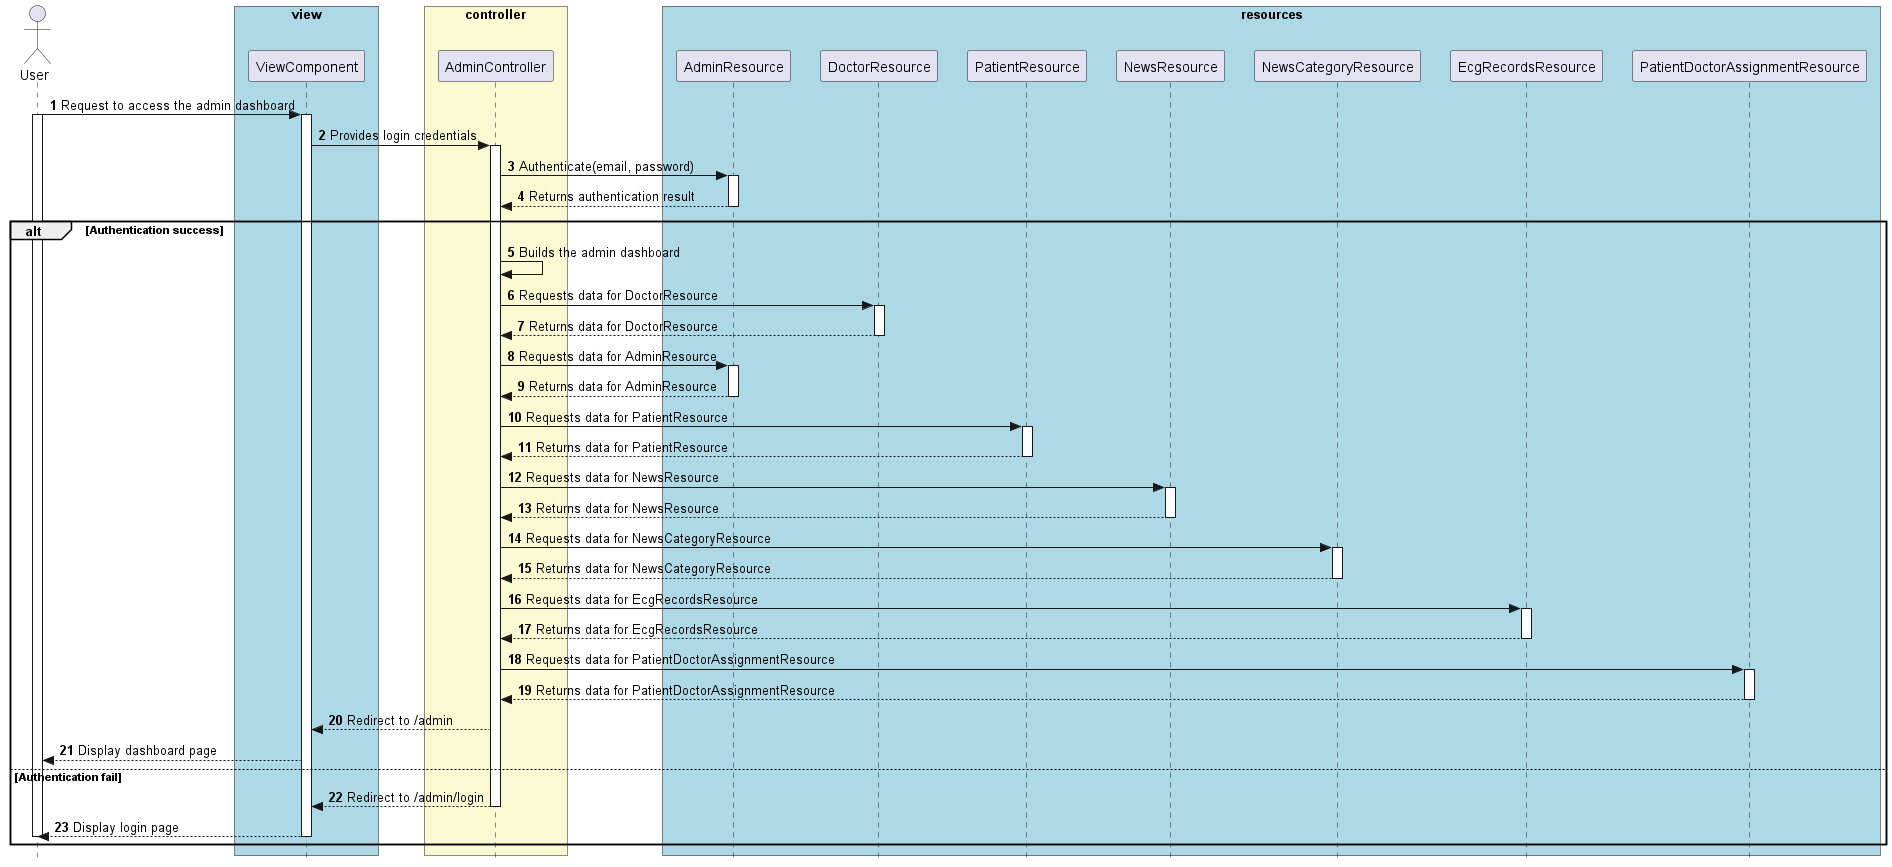
\includegraphics[width=16cm,height=10cm]{Images/server/sequence/web/seq_auth.png}
  \caption[Sơ đồ tuần tự cho quá trình truy cập vào trang quản trị (admin dashboard) ]{\bfseries \fontsize{12pt}{0pt}
  \selectfont Sơ đồ tuần tự cho quá trình truy cập vào trang quản trị (admin dashboard) }
  \label{seq_auth} %đặt tên cho ảnh
\end{figure}
Hình \ref{seq_auth} mô tả quá trình truy cập vào bảng điều khiển quản trị (admin dashboard) của người dùng (User). Khi người dùng yêu cầu truy cập vào admin dashboard, hệ thống sẽ yêu cầu xác thực thông qua ViewComponent. Nếu xác thực thành công, AdminJS sẽ xây dựng admin dashboard và yêu cầu dữ liệu từ các tài nguyên (resources) khác nhau để hiển thị thông tin.



Nếu xác thực thành công, AdminJS sẽ yêu cầu dữ liệu từ các tài nguyên khác nhau, bao gồm DoctorResource, AdminResource, PatientResource, NewsResource, NewsCategoryResource, EcgRecordsResource và PatientDoctorAssignmentResource. Mỗi tài nguyên sẽ trả về dữ liệu tương ứng và AdminJS sẽ sử dụng các dữ liệu này để hiển thị trên admin dashboard.



Sau khi AdminJS đã thu thập đủ dữ liệu từ các tài nguyên, nó sẽ chuyển hướng ViewComponent đến trang /admin để hiển thị admin dashboard cho người dùng. Nếu xác thực không thành công, AdminJS sẽ chuyển hướng ViewComponent đến trang /admin/login để hiển thị trang đăng nhập cho người dùng.



Sau khi hoàn tất, hệ thống sẽ trả về response cuối cùng và hiển thị trang tương ứng cho người dùng.


\begin{figure}[H]
  \centering
  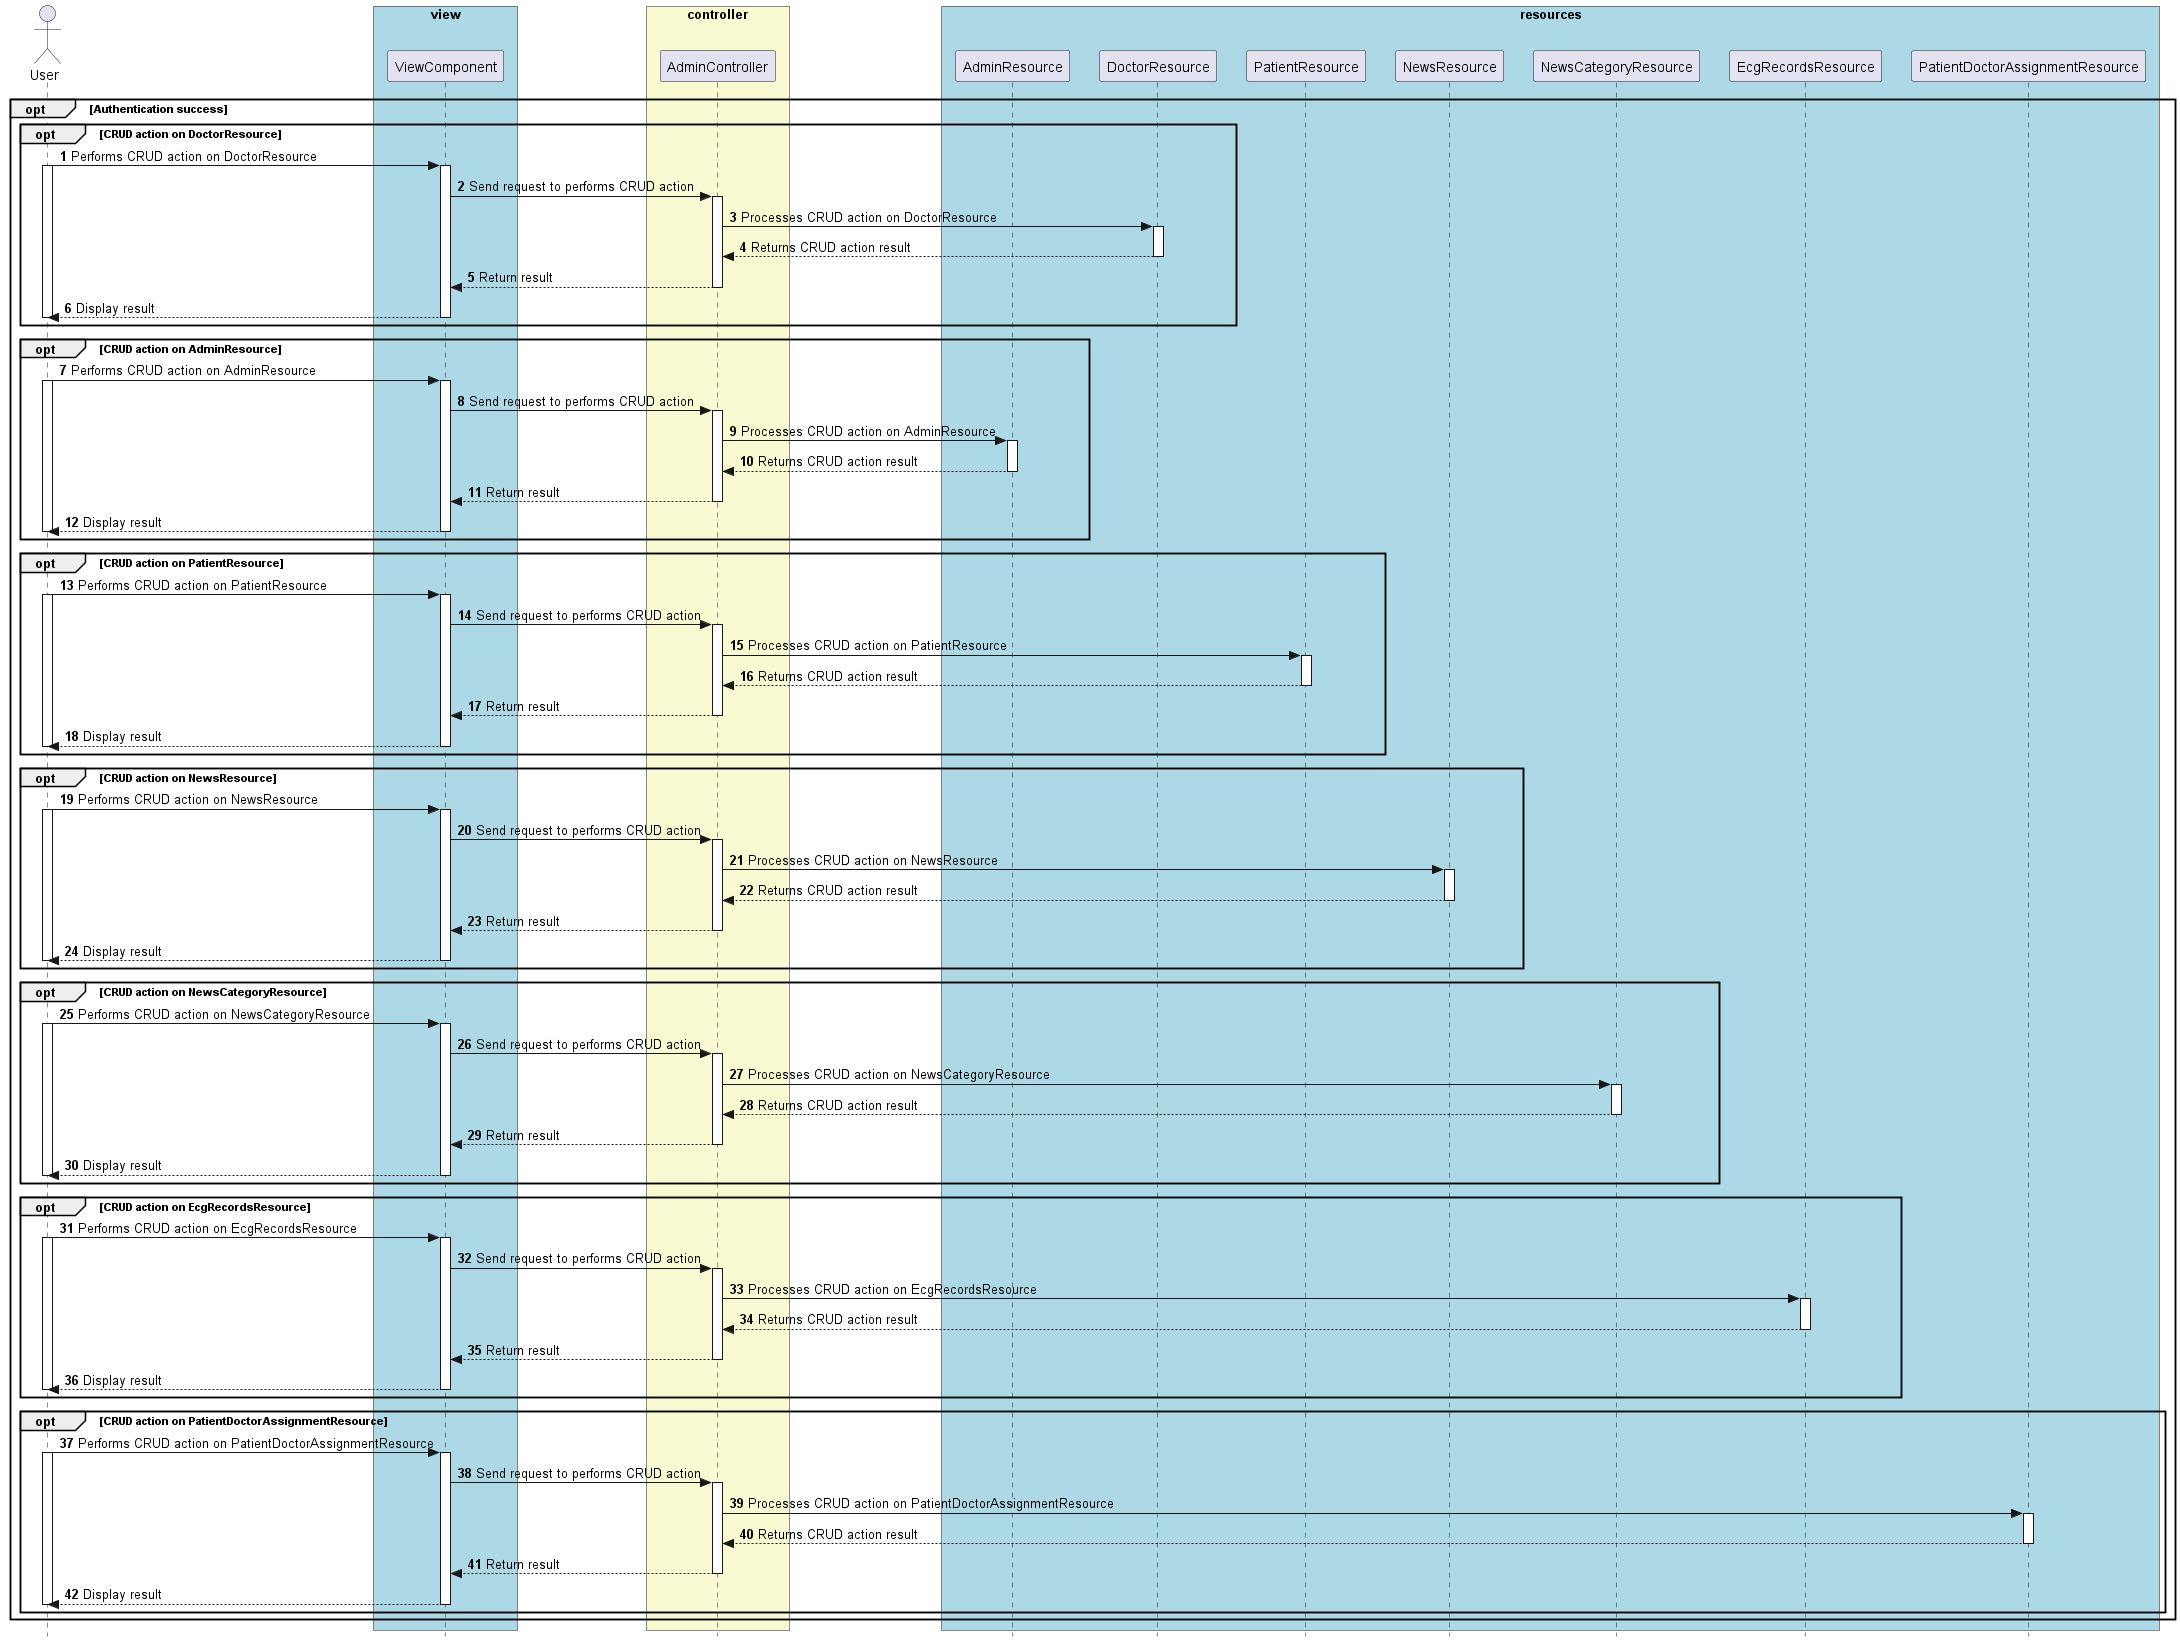
\includegraphics[width=16cm,height=14cm]{Images/server/sequence/web/seq_crud.png}
  \caption[Sơ đồ tuần tự cho quá trình trình thực hiện các thao tác CRUD trên các tài nguyên (resources) ]{\bfseries \fontsize{12pt}{0pt}
  \selectfont Sơ đồ tuần tự cho quá trình trình thực hiện các thao tác CRUD trên các tài nguyên (resources) }
  \label{seq_crud} %đặt tên cho ảnh
\end{figure}
Hình \ref{seq_crud}  mô tả quá trình thực hiện các thao tác CRUD trên các tài nguyên (resources) khác nhau của admin dashboard khi người dùng (User) thực hiện các thao tác trong ViewComponent.


Khi người dùng thực hiện các thao tác CRUD trên các tài nguyên, hệ thống sẽ xác thực người dùng trước đó. Sau khi xác thực thành công, người dùng sẽ thực hiện các thao tác CRUD trên ViewComponent, và ViewComponent sẽ gửi yêu cầu thực hiện thao tác tương ứng tới AdminJS.


Sau đó, AdminJS sẽ thực hiện thao tác CRUD tương ứng trên các tài nguyên, bao gồm DoctorResource, AdminResource, PatientResource, NewsResource, NewsCategoryResource, EcgRecordsResource và PatientDoctorAssignmentResource. Mỗi tài nguyên sẽ xử lý yêu cầu và trả về kết quả tương ứng cho AdminJS.


Sau khi AdminJS đã nhận được kết quả từ các tài nguyên, nó sẽ trả về kết quả đó cho ViewComponent. ViewComponent sẽ hiển thị kết quả tương ứng cho người dùng. Quá trình này được thực hiện đối với từng tài nguyên mà người dùng yêu cầu thực hiện thao tác CRUD.



\subsubsection{Thiết kế các chức năng chính cho ứng dụng di động}
\label{design_function_mobile}

Ứng dụng di động được trong hệ thống được chia cụ thể gồm ứng dụng di động cho bệnh nhân và ứng dụng di động cho bác sĩ. 
Hầu hết các chức năng cơ bản được thể hiện trong sơ đồ usecase của hai ứng dụng đều giống nhau như đăng nhập, xem lịch sử đo, nhắn tin.
Điểm khác biệt giữa hai ứng dụng di động là ứng dụng di động cho bệnh nhân sẽ có thêm chức năng kết nối với thiết bị đo cũng như xem tin tức.

Trong nội dung của mục \ref{design_function_mobile}, chúng em xin được phép trình bày chi tiết hướng thực hiện các chức năng
từ các chức năng chung đến chức năng riêng cho bệnh nhân, đồng thời sẽ triển khai hướng tối ưu của từng chức năng (nếu có).

Các chức năng chung của hai ứng dụng bao gồm: 
\begin{itemize}
  \item Chức năng đăng nhập
  \item Chức năng xem lịch sử đo
  \item Chức năng nhắn tin.
\end{itemize}

Các chức năng riêng của bệnh nhân bao gồm:
\begin{itemize}
  \item Chức năng kết nối và thực hiện đo với thiết bị điện tim
  \item Chức năng xem tin tức.
\end{itemize}

\paragraph{Chức năng đăng nhập}
\mbox{}

Chức năng đăng nhập là chức năng chung của hai ứng dụng, có tương tác trực tiếp với API, logic cơ bản được thể hiện ở Hình \ref{login}
luồng thực hiện ở phía server được triển khai ở 
Hình \ref{backend_login}. Có thể nhận thấy việc đăng nhập trên App chỉ nên diễn ra một lần sau khi người dùng nhập thông tin,
và đã được xác thực. Bởi mỗi lần tắt đi bật lại ứng dụng, nếu phải đăng nhập lại thì rất phiền cho người sử dụng, đặc biệt
với những ứng dụng không đòi hỏi tính truy nhập và bảo mật quá cao. Có nhiều cách để lưu dữ liệu đăng nhập như:

\begin{itemize}
  \item Lưu ở bộ nhớ ngoài: Mỗi lần mở app sẽ kiểm tra dữ liệu trong file. Nếu khớp với điều kiện đặt ra sẽ cho người dùng vào thẳng app.
  Tuy nhiên cách này khá rườm rà và yêu cầu người thực hiện phải truy xuất file nhiều.
  \item Lưu trên server: Mỗi lần mở app sẽ đẩy một yêu cầu lên server và server sẽ trả về trạng thái. Tuy nhiên, như vậy mọi tác
  vụ sẽ phụ thuộc hoàn toàn vào internet. Và nếu số lượng người sử dụng lớn thì hoàn toàn không phù hợp.
  \item Lưu trong bộ nhớ cục bộ của ứng dụng: Các hệ điều hành đều cung cấp những thư viện giúp việc lưu trữ dữ liệu nhỏ một cách 
  dễ dàng trong cục bộ ứng dụng. Đây là một phương pháp lưu dưới dạng key-value (khoá-giá trị), giúp việc truy/xuất hay ghi nhanh chóng.
  Với Android, chúng ta có thể sử dụng SharedPreferences (thêm tham khảo), với IOS là UserDefault (thêm tham khảo)
  % //TODO: thêm tham khảo sharepref

\end{itemize}
Vậy luồng đăng nhập và lưu dữ liệu đăng nhập trên ứng dụng di động sẽ là: người dùng nhập thông tin, thông tin được gửi lên server xác thực,
nếu kết quả trả về của server là đúng, sẽ lưu dữ liệu đăng nhập của người dùng vào trong Shared Preferences (Local Storage). Khi tắt và mở lại app,
ứng dụng sẽ lấy dữ liệu và kiểm tra, nếu có dữ liệu thì người dùng sẽ không phải đăng nhập lại. Hình dưới mô tả chi tiết phần thiết
kế việc lưu dữ liệu đăng nhập.

\begin{figure}[H]
  \centering
  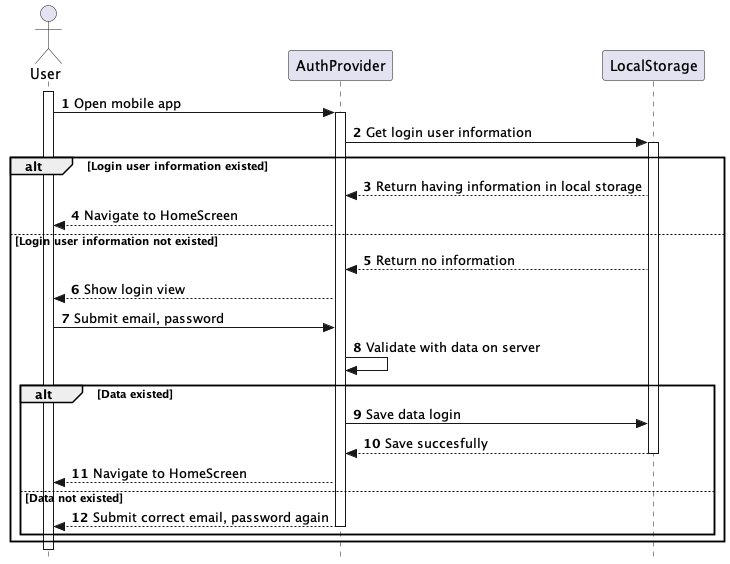
\includegraphics[width=16cm,height=10cm]{Images/mobile_app/design_store_data_login.png}
  \caption[Sơ đồ tuần tự phần thiết kế chức năng đăng nhập và lưu dữ liệu đăng nhập]{\bfseries \fontsize{12pt}{0pt}
  \selectfont Sơ đồ tuần tự phần thiết kế chức năng đăng nhập và lưu dữ liệu đăng nhập}
  \label{seq_auth} %đặt tên cho ảnh
\end{figure}

\paragraph{Chức năng kết nối và nhận dữ liệu từ thiết bị điện tim}
\mbox{}

Chức năng kết nối và nhận dữ liệu từ thiết bị điện tim là một trong những chức năng quan trọng nhất của ứng dụng. Chức năng này yêu cầu
ứng dụng phải bật được bluetooth. Đầu tiên để có thể tiến hành đo, chúng ta phải thực hiện một kết nối bluetooth giữa ứng dụng di động và
thiết bị đo điện tim. Sau khi dã kết nối thành công, dựa vào cơ chế của bluetooth low energy, chúng ta sẽ thiết lập để ứng dụng lắng
nghe dữ liệu trả ra từ thiết bị điện tim. Dữ liệu thô được xử lý theo công thức tính toán và sau đó được vẽ trên biểu đồ. Người dùng sau
khi thực hiện đo xong có thể chọn lưu kết quả đo lại (điều này sẽ đẩy dữ liệu đo lên server và bác sĩ có thể xem được).
% //TODO: add reference
% https://learn.adafruit.com/introduction-to-bluetooth-low-energy/gatt

Đầu tiên việc kết nối Bluetooth với thiết bị đo điện tim là không khó khi có sự hỗ trợ của các thư viện và hệ điều hành, sau đó việc xử lý sau
kết nối mới là một điều chúng ta cần phải lưu tâm tới. Sau khi kết nối với thiết bị đo điện tim, câu hỏi đặt ra là \textbf{làm thế nào
để lắng nghe được dữ liệu} từ thiết bị điện tim? Đối với hệ thống BLE, sau khi kết nối thành công, một Profile Protocol được gọi
là GATT (Generic ATTribute Profile) - xác định cách hai thiết bị sẽ truyền và nhận dữ liệu như thế nào thông qua
Services và Characteristics sẽ được hình thành. 
% //TODO: Chèn ảnh vào đây ảnh gatt
Services là tập hợp của một nhóm thông tin để thực hiện một chức năng cụ thể,
ví dụ Battery Service, Sensor Service, trong mỗi Service chính là một hoặc nhiều Characteristic, mỗi Characteristic đảm nhận
một thông tin hoặc chức năng riêng biệt phục vụ cho Service đó. Mỗi một Service hay Characteristic đều có UUID (mã định danh duy nhất toàn cầu).

Từ cơ sở trên, để có thể sẵn sàng lắng nghe được dữ liệu từ thiết bị điện tim, thiết bị di động cần kết nối đến đúng Services và Characteristics.

Trong thiết bị đo thực hiện trong đồ án lần này, chúng em xác định được những UUID tiêu chuẩn (biểu diễn dưới dạng String) để có thể lắng nghe được dữ liệu từ
thiết bị:
\begin{itemize}
  \item UUID Service: 6E400001-B5A3-F393-E0A9-E50E24DCCA9E
  \item UUID Characteristic: 6E400003-B5A3-F393-E0A9-E50E24DCCA9E
\end{itemize}

\begin{figure}[H]
  \centering
  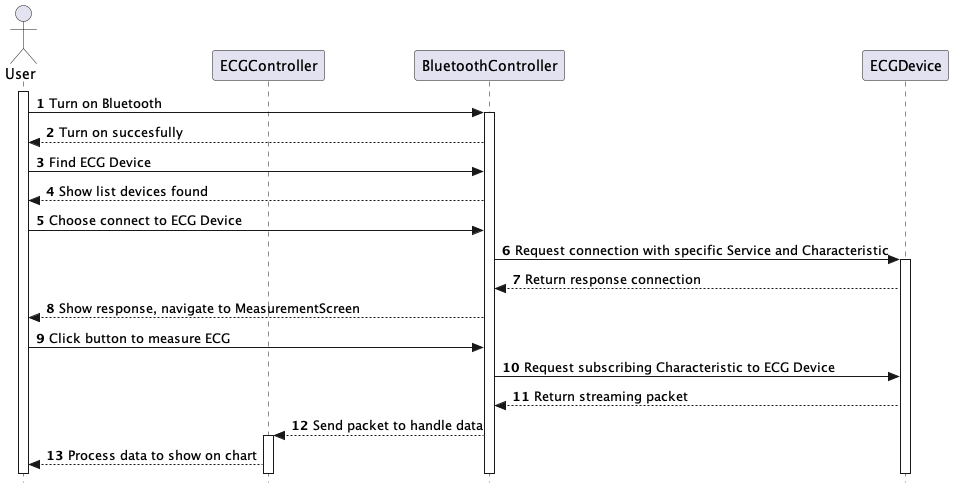
\includegraphics[width=16cm,height=10cm]{Images/mobile_app/design_connect_and_receive_ECG_data.png}
  \caption[Sơ đồ tuần tự thiết kế chức năng kết nối và nhận dữ liệu điện tim real-time]{\bfseries \fontsize{12pt}{0pt}
  \selectfont Sơ đồ tuần tự thiết kế chức năng kết nối và nhận dữ liệu điện tim real-time}
  \label{seq_auth} %đặt tên cho ảnh
\end{figure}

Sau khi hoàn thành phần xây dựng kết nối với thiết bị đo điện tim, quá trình thực hiện đo được bắt đầu. Ứng dụng sẽ lắng nghe
dữ liệu từ thiết bị thông qua một hàm "subscribe characteristic", dữ liệu sẽ gửi liên tục qua characteristic này. Nhiệm vụ sau đó của ứng dụng là
định nghĩa gói dữ liệu, xử lý và chuẩn hoá số liệu, từ đó vẽ lên biểu đồ. Chi tiết về bước định nghĩa gói dữ liệu, xử lý số liệu sẽ được chúng em trình bày
ở chương sau. 
% //TODO: add hình THêm luồng xử lý dữ liệu và lưu file

Sau mỗi lần đo, dữ liệu sẽ được gửi lên server để lưu trữ và hiển thị lại cho bệnh nhân/bác sĩ quản lý xem nếu cần. Việc xem
lịch sử đo được chúng em tiếp tục trình bày ở mục \ref{function_view_history_record}.

\paragraph{Chức năng xem lịch sử đo}
\label{function_view_history_record}
\mbox{}

Chức năng xem lịch sử đo lấy dữ liệu trực tiếp trên server, với logic cơ bản được thể hiện ở Hình \ref{view_record_timeline}. 
Để xem được lịch sử các lần đo, bệnh nhân cần thực hiện đo ít nhất một lần (hệ thống sẽ tự gửi dữ liệu lên server). Dữ liệu sau khi được
load từ API về sẽ được vẽ lên biểu đồ. Các Hình \ref{getEcgRecordsByDoctor}, Hình \ref{getEcgRecordsByUserId}
lần lượt thể hiện luồng API hoạt động ở server để lấy dữ liệu về danh sách các phiên đo. 

Trong các API trên hoàn toàn chưa có dữ liệu chính của phiên đo, chỉ khi người dùng chọn một phiên đo muốn xem, lúc đó dữ liệu
mới được tải về từ server (thể hiện trong Hình \ref{convertExceltoJson}). Dữ liệu sau khi được lấy về sẽ được vẽ lên biểu đồ giống
như biểu đồ theo dõi dữ liệu điện tim real-time.

Biểu đồ có trục tung là giá trị điện áp, trục hoành là toàn bộ thời gian từ lúc bắt đầu đo đến khi kết thúc. Người dùng có thể,
thực hiện các thao tác phóng to, thu nhỏ để xem khoảng thời gian.

\paragraph{Chức năng xem tin tức}
\mbox{}

Chức năng xem tin tức lấy dữ liệu trực tiếp trên server, với logic cơ bản được thể hiện ở Hình \ref{view_news}. 
Danh sách tin tức sẽ được load ngay khi người dùng mở ứng dụng (nếu có mạng). Tất cả phần xem trước của tin tức sẽ được lưu
trong biến khi ứng dụng chạy, dữ liệu tin tức được lấy từ danh sách tin tức không bao gồm nội dung để giảm thiểu khối lượng
thông tin dư thừa của gói tin. Chỉ khi người dùng chọn một tin tức cụ thể, khi đó ứng dụng mới gửi yêu cầu lên server để lấy
nội dung tin tức đó về, nội dung tin tức được chúng em thống nhất lưu dưới dạng HTML và khi hiện lên sẽ hiển thị dạng HTML view.
Điều này giúp cấu trúc của thông tin được nguyên vẹn và không cần phải chỉnh sửa nhiều.

% //TODO: Thêm ảnh demo chức năng, hoặc biểu đồ giải thích xem tin tức, ảnh html

\paragraph{Chức năng nhắn tin}
\mbox{}

Chức năng nhắn tin là chức năng được thiết kế để không phụ thuộc vào server của hệ thống mà độc lập đứng riêng. Chúng em
chọn Firebase làm nền tảng để phát triển chức năng nhắn tin bởi tính phổ biến, hỗ trợ rất nhiều ngôn ngữ đi kèm với tài liệu đầy đủ 
và dễ dàng phát triển.
Ở chức năng nhắn tin, mọi dữ liệu về tin nhắn sẽ được lưu trên Firestore (Cơ sở dữ liệu NoSQL của Firebase), cơ sở dữ liệu sẽ
bao gồm ba bảng chính. 
% //TODO: Thêm các bảng tin nhắn và giải thích ở chương 2

Việc xử lý tin nhắn, gửi tin nhắn, hay các thao tác với tin nhắn đều có thể sử dụng các câu lệnh truy vấn và truy/xuất
trực tiếp vào cơ sở dữ liệu, đồng thời các ví dụ và câu lệnh được Firebase hỗ trợ rất kĩ về mặt tài liệu, vì lẽ đó, khi sử dụng
Firebase, ứng dụng sẽ linh hoạt và dễ cải tiến.

Ví dụ, ứng dụng di động đang trong giao diện trò chuyện, tức nghĩa là phải có một câu truy vấn lấy các tin nhắn trong hội thoại
để hiển thị cho người dùng. Khi gửi tin nhắn, một hàng được thêm vào
cơ sở dữ liệu, tuỳ theo cơ chế của ngôn ngữ lập trình, Firebase lắng nghe được sự thay đổi
trong cơ sở dữ liệu và lập tức gửi một thông điệp đến ứng dụng để cho người dùng biết, đồng thời cập nhật tin nhắn kèm giao diện.

% //TODO: Thêm ảnh demo và hỏi anh Tuấn cách thêm notes
\begin{figure}[H]
  \centering
  \includegraphics[width=16cm,height=10cm]{Images/mobile_app/design_send_receive_message.png}
  \caption[Sơ đồ tuần tự thiết kế chức năng gửi và nhận tin nhắn real-time]{\bfseries \fontsize{12pt}{0pt}
  \selectfont Sơ đồ tuần tự thiết kế chức năng gửi và nhận tin nhắn real-time}
  \label{design_send_receive_firebase_message} %đặt tên cho ảnh
\end{figure}

Hình \ref{design_send_receive_firebase_message} biểu diễn chi tiết cách gửi/nhận tin nhắn thông qua Firebase. Khi người dùng,
gửi một tin nhắn thông qua FirebaseMessagesController, dữ liệu được lưu vào trong FirebaseDatabase, ngay lúc đó, Firebase sẽ có
cơ chế thông báo cho người dùng đã thực hiện query ở luồng 6, có một tin nhắn mới được thêm. Ứng dụng có thể nhận được tin nhắn
đó ngay lập tức và hiển thị lên màn hình.

\subsubsection{Kết luận chương}

\newpage